\part{Grundlagen}
\chapter{Gleichungen}
\begin{inhalt}
  Lösen von Gleichungen mit
  \begin{itemize}
    \item Äquivalenzumformungen
    \item Mitternachtsformel
    \item Satz vom Nullprodukt
    \item Substitution
  \end{itemize}
\end{inhalt}

\ \\

Eine \emph{Gleichung} sagt aus, dass zwei Terme\sidenote{Ein \textbf{Term} ist ein Rechenausdruck, der aus Zahlen, Rechenzeichen und Klammern bestehen kann.} gleich sind. Meistens hängen diese
von einer Variable --- zum Beispiel $x$ --- ab. Es gilt herauszufinden, für welche $x$ die Gleichung erfüllt ist:
\begin{equation*}
  x^2+1=10\ \Rightarrow\ x=\pm 3, \text{ denn } {(\pm 3)}^2+1=9+1=10
\end{equation*}

\begin{bla}{Äquivalenzumformungen}
  \begin{marginfigure}[3em]
    \begin{tcolorbox}[colback=white!95!black,colframe=white!75!black,title=CAS:,arc=0mm]
      \begin{scriptsize}
        \textbf{Calculator}: \\*
        \menu{Menü > Algebra > Lösen}
        \begin{flushright}
          \( \text{\textsc{solve}}(5x+4 = 3x-2 \ , \ x) \) \\*
          \( \bm{\leadsto x = -3} \)
        \end{flushright}
      \end{scriptsize}
    \end{tcolorbox}
  \end{marginfigure}
  Bei einer \emph{Äquivalenzumformung} wird auf beiden Seiten der Gleichung dasselbe gemacht.
  \\
  \textbf{Achtung}: Wenn du auf beiden Seiten die Wurzel ziehst, dann vergiss nicht, dass jede Zahl zwei Wurzeln hat! \\
  \begin{equation*}
    \begin{alignedat}{4}
                        && 5x+4 & = 3x-2 & \quad & | -4 \\
      \Leftrightarrow\  && 5x   & = 3x-6 & \quad & | -3x \\
      \Leftrightarrow\  && 2x   & = -6   & \quad & | *\tfrac{1}{2} \\
      \Leftrightarrow\  && x    & = -3
    \end{alignedat}
  \end{equation*}
\end{bla}



\begin{bla}{Lösen von quadratischen Gleichungen: die Mitternachtsformel}
  \begin{marginfigure}[7em]
    \begin{tcolorbox}[colback=white!95!black,colframe=white!75!black,title=CAS:,arc=0mm]
      \begin{scriptsize}
        \textbf{Calculator}: \\*
        \menu{Menü > Algebra > Nullstellen}
        \begin{flushright}
          \( \text{\textsc{zeros}}(3x^2-3 \ , \ x) \) \\*
          \( \bm{\leadsto \{ -1, 1 \}} \)
        \end{flushright}
      \end{scriptsize}
    \end{tcolorbox}
  \end{marginfigure}
  Gleichungen der Form $ax^2+bx+c=0$ ($a,b$ und $c$ sind hierbei beliebige Zahlen, können also auch Null sein) können mit der \emph{Mitternachtsformel}
  gelöst werden. Man erhält \textbf{zwei} Ergebnisse $x_1$ und $x_2$, indem man für $\pm$ einmal $+$ und einmal $-$ rechnet:
  \begin{equation*}
    x_{1,2}=\frac{-b\pm \sqrt{b^2-4ac}}{2a}
  \end{equation*}
  Das funktioniert so:
  \begin{equation*}
    \begin{alignedat}{4}
                        && 2x          & = x^2-3                                    & \quad & |\ +3 \\
      \Leftrightarrow\  && 2x+3        & = x^2                                      & \quad & |\ -x^2 \\
      \Leftrightarrow\  && -x^2+2x+3   & = 0                                        & \quad & |\ \text{MNF:\ } a=-1, b=2, c=3 \\
      \Leftrightarrow\  && x_{1,2}     & = \frac{-2\pm \sqrt{2^2-4*(-1)*3}}{2*(-1)} & \quad & \\
      \Leftrightarrow\  && x_{1,2}     & = \frac{-2 \pm 4}{-2}                      & \quad & \\
    \end{alignedat}
  \end{equation*}
  Wir erhalten also $x_1 = -1$ und $x_2 = 3$.
\end{bla}



\begin{bla}{Satz vom Nullprodukt}
  Das Produkt von zwei Termen ist genau dann Null, wenn mindestens einer der beiden Terme Null ist.
  Liegt also eine Gleichung der Form
  \begin{equation*}
    (\text{Term}_1)*(\text{Term}_2)=0
    \end{equation*}
  vor, so können die beiden Terme einzeln betrachtet werden. Man betrachtet $(\text{Term}_1)=0$ und $(\text{Term}_2)=0$. Es gibt deswegen meistens zwei Möglichkeiten für $x$, die die Gleichung erfüllen:
  \begin{equation*}
    (x-1)(x-3) = 0
  \end{equation*}
  hat also die Lösungen $x=1$ und $x=3$, da genau dann einer der beiden Terme Null ist.
\end{bla}

\begin{bla}{Substitution}
  Manche Gleichungen lassen sich nicht durch die bisher bekannten Hilfsmittel lösen, zum Beispiel, weil Potenzen von $x$ mit einem Exponenten $>2$ vorkommen. Eine Möglichkeit solche Gleichungen zu lösen bietet das \emph{Substituieren}. Hierbei wird ein Term durch eine Variable abgekürzt und die
  so vereinfachte Gleichung gelöst. Danach macht man das Abkürzen rückwärts und erhält so die Ergebnisse der ursprünglichen Gleichung:
  \begin{align*}
    x^4+11x^2+10 & = 0 \\
    \text{Substitution:}\ z & = x^2 \\
    \rightsquigarrow z^2+11z+10 & = 0 \\
    \text{Man erhält mit der MNF}: z_1 & = -10, z_2=-1 \\
    \text{Rücksubstitution}\ x_1: x_1^2 & = z_1=-10 \\
    \text{Rücksubstitution}\ x_2: x_2^2 & = z_2=-1 \\
  \end{align*}
  Die Gleichung hat also keine Lösung, da es keine reellen Zahlen gibt, deren Quadrat kleiner Null ist.
\end{bla}

\chapter{Rechenregeln}

\begin{inhalt}
  Wichtige Rechenregeln, die man können muss:
  \begin{itemize}
    \item KlaHoPS
    \item Brüche
    \item Wurzeln
    \item Potenzen
    \item Logarithmen
  \end{itemize}
\end{inhalt}

\begin{bla}{KlaHoPS}
  Die wohl fundamentalste Regel ist die Reihenfolge, in der man Rechenoperationen durchführt. Es gilt:
  \begin{enumerate}
    \item Inhalt der innersten Klammer ausrechnen (hier gilt natürlich auch diese Rechenreihenfolge)
    \item Hochzahlen ausrechnen
    \item Punkt vor Strich
  \end{enumerate}
  Man merkt sich: \textbf{Klammer, Hochzahl, Punkt vor Strich}, kurz \textbf{KlaHoPS} (ja, das hört sich komisch an).
\end{bla}

\begin{bla}{Brüche}
  \begin{itemize}
    \item \textbf{Kürzen}: Beim Kürzen eines Bruchs versucht man, Zähler und Nenner möglichst klein zu machen. Das macht man, indem man Zähler und Nenner jeweils durch dieselbe Zahl teilt: $ \frac{9}{3}=\frac{9:3}{3:3}=\frac{3}{1}=3$
    \item \textbf{Erweitern}: Erweitern ist Kürzen rückwärts: statt Zähler und Nenner durch eine Zahl zu teilen multipliziert man sie mit derselben Zahl: \\$\frac{2}{5}=\frac{2*2}{5*2}=\frac{4}{10}$
    \item \textbf{Auf gleichen Nenner bringen}: Hat man zwei Brüche gegeben und möchte sie auf denselben Nenner bringen, so erweitert man beide Brüche so, dass sie denselben Nenner haben. Man kann beispielsweise den ersten Bruch mit dem Nenner vom zweiten Bruch und den zweiten Bruch mit dem Nenner vom ersten Bruch erweitern: \\ $\frac{2}{3}=\frac{2*4}{3*4}=\frac{8}{12} \qquad \frac{3}{4}=\frac{3*3}{4*3}=\frac{9}{12}$
    \item \textbf{Addieren}: Man addiert Brüche, indem man sie auf denselben Nenner bringt und dann ihre Zähler addiert: $\frac{a}{b}+\frac{c}{d} = \frac{a*d}{b*d}+\frac{c*b}{b*d} = \frac{a*d+c*b}{b*d}$
    \item \textbf{Subtrahieren}: Man subtrahiert Brüche, indem man sie auf denselben Nenner bringt und dann ihre Zähler subtrahiert:
    \\$\frac{a}{b}-\frac{c}{d} = \frac{a*d}{b*d}-\frac{c*b}{b*d} = \frac{a*d-c*b}{b*d}$
    \item \textbf{Multiplizieren}: Man multipliziert Brüche, indem man jeweils die Zähler und die Nenner miteinander multipliziert: $\frac{a}{b}*\frac{c}{d}=\frac{a*c}{b*d}$
    \item \textbf{Dividieren}: Man dividiert Brüche, indem man den ersten Bruch mit dem Kehrwert des zweiten Bruchs multipliziert: $\frac{a}{b}:\frac{c}{d}=\frac{a}{b}*\frac{d}{c}=\frac{a*d}{b*c}$
  \end{itemize}
\end{bla}

\begin{bla}{Wurzeln}
  \begin{itemize}
    \item \textbf{Multiplikationsregel}: $\sqrt{a*b}=\sqrt{a}*\sqrt{b}$
    \item \textbf{Divisionsregel}: $\sqrt{\frac{a}{b}}=\frac{\sqrt{a}}{\sqrt{b}}$
    \item \textbf{Teilweise Wurzel ziehen}: Manchmal kann man eine Wurzel teilweise ziehen, indem man die Multiplikationsregel anwendet: $\sqrt{32*x^2}=\sqrt{32}*\sqrt{x^2}=\sqrt{16*2}*\sqrt{x^2}=4*\sqrt{2}*\sqrt{x^2}=4*|x|*\sqrt{2}$.
    \\Der Betrag kommt daher, dass $x^2$ für jedes $x$ positiv ist, deswegen ist $\sqrt{x^2}$ auch wieder positiv.
  \end{itemize}
\end{bla}

\begin{bla}{Potenzgesetze}
  \begin{itemize}
    \item $a^0=1$
    \item $a^{-r}=\frac{1}{a^r}$
    \item $a^{\frac{1}{n}}=\sqrt[n]{a}$, insbesondere $a^{\frac{1}{2}}=\sqrt{a}$
    \item $a^{r+s}=a^r*a^s$
    \item $a^{r-s}=a^{r+(-s)}=a^r*a^{-s}=a^r*\frac{1}{a^s}=\frac{a^r}{a^s}$
    \item ${(a*b)}^r=a^r*b^r$
    \item ${(\frac{a}{b})}^r=\frac{a^r}{b^r}$
    \item ${(a^r)}^s=a^{r*s}$
  \end{itemize}
\end{bla}

\begin{bla}{Logarithmengesetze}
  Mehr zum Umgang mit dem Logarithmus und der natürlichen Exponentialfunktion findet ihr im Kapitel zu Exponentialfunktionen.
  \begin{itemize}
    \item $\ln(u*v)=\ln(u)+\ln(v)$
    \item $\ln(\frac{u}{v})=\ln(u)-\ln(v)$
    \item $\ln(u^k)=k*\ln(u)$
  \end{itemize}
  $\ln(x)$ steht hierbei für den natürlichen Logarithmus, also den Logarithmus zur Basis $e$ ($\log_e(x)$). Eine weitere oft verwendete Basis ist $10$ (das bedeutet, dass $\log_{10}(10^x)=x=\lg(x)$). Mann kann von einer Basis $a$ zu einer Basis $b$ wechseln:
  \begin{equation*}
    \log_b(x)=\frac{\log_a(x)}{\log_a(b)}
  \end{equation*}
\end{bla}

\chapter{Funktionen}

\begin{inhalt}
  Funktionen und ihre Eigenschaften:
  \begin{itemize}
    \item Definition Funktionsbegriff
    \item Wichtige Funktionen
    \item Eigenschaften (Achsenschnittstellen, Monotonie, Grenzwerte)
    \item Trigonometrische Funktionen
  \end{itemize}
\end{inhalt}

\section{Grundlegende Eigenschaften}

\begin{bla}{Funktion}
  Eine \emph{Funktion} ist etwas, das einer Zahl ($x$) eine andere ($f(x)$) zuordnet. $f(x)=x^2$ ordnet beispielsweise einer Zahl $x$ ihr Quadrat, also $x^2$, zu. \\
  Wir können eine Funktion graphisch veranschaulichen, indem wir sie in ein Koordinatensystem zeichnen.

  \begin{marginfigure}
    \begin{tikzpicture}[
        scale=0.7,
        thick,
        >=stealth',
        dot/.style = {
          draw,
          fill = white,
          circle,
          inner sep = 0pt,
          minimum size = 4pt
        }
      ]
      \coordinate (O) at (0,0);

      \draw[step=1cm,gray!40] (-2.9,-0.9) grid (2.9,2.9);

      % Achsen
      \draw[->] (-3,0) -- (3,0) coordinate[label = {below:$x$}] (xmax);
      \draw[->] (0,-1) -- (0,3) coordinate[label = {right:$f(x)$}] (ymax);

      % Graph
      \draw[domain=-2:2,smooth,variable=\x,red, label={right:$f$}] plot ({\x},{\x*\x});
      \draw (2,3.5) node[red,label= {[red]below:$f$}] {};

      % y-Wert
      \draw (1,1) -- (-0.1, 1) node[label = {left:\footnotesize $f(x_0)$}] {};

      % x-Wert und marker
      \draw (1,1) node[dot] {} -- (1,-0.1) node[label = {below:\footnotesize $x_0$}] {};
    \end{tikzpicture}
    \caption{Graph von $f(x)=x^2$. Für einen $x$-Wert von der $x$-Achse (hier $x_0$) kann sein zugehöriger $f(x)$-Wert (hier $f(x_0)$) abgelesen werden.}
  \end{marginfigure}
  \begin{marginfigure}
    \begin{tcolorbox}[colback=white!95!black,colframe=white!75!black,title=CAS:,arc=0mm]
      \begin{scriptsize}
        \textbf{Calculator}: \hfill \( f(x) := |x| \) \\* \ \\*
        \textbf{Graph}: \hfill \( f1(x) = f(x) \)
      \end{scriptsize}
    \end{tcolorbox}
  \end{marginfigure}
\end{bla}

\begin{bla}{Punkt, Stelle, Wert}
  \begin{itemize}
    \item \textbf{Punkt}: Ein Punkt ist ein Zahlenpaar, bestehend aus $x$- und $y$-Wert.
    \item \textbf{Stelle, Wert}: An der \emph{Stelle} $x_0$ hat $f$ den \emph{Wert} $f(x_0)$. Das ergibt den \emph{Punkt} $\mathrm{P}(x_0|f(x_0))$.
  \end{itemize}
\end{bla}

\begin{bla}{Wichtige Funktionen: Betragsfunktion}
  \begin{marginfigure}
    \begin{tikzpicture}[
        scale=0.7,
        thick,
        >=stealth',
        dot/.style = {
          draw,
          fill = white,
          circle,
          inner sep = 0pt,
          minimum size = 4pt
        }
      ]
      \coordinate (O) at (0,0);

      \draw[step=1cm,gray!40] (-2.9,-0.1) grid (2.9,2.9);

      % Achsen
      \draw[->] (-3,0) -- (3,0) coordinate[label = {below:$x$}] (xmax);
      \draw[->] (0,-0.1) -- (0,3) coordinate[label = {right:$f(x)$}] (ymax);

      % Graph
      \draw[domain=-2:0,smooth,variable=\x,red, label={right:$f$}] plot ({\x},{-\x});
      \draw[domain=0:2,smooth,variable=\x,red, label={right:$f$}] plot ({\x},{\x});

      \draw (2,2.8) node[red,label= {[red]below:$|x|$}] {};
    \end{tikzpicture}
    \caption{Graph von $f(x)=|x|$.}
  \end{marginfigure}

  Der \emph{Betrag} $f(x)=|x|$ einer Zahl ist der Abstand der Zahl zum Ursprung auf der Zahlengeraden. Der Betrag hebt also quasi ein $-$ als Vorzeichen auf: $|-5|=5, |3|=3$. Formal gilt:
  \begin{align*}
    |x|=\begin{cases}
        x\  & \text{falls $x\geq 0$} \\
        -x\  & \text{falls $x<0$}
    \end{cases}
  \end{align*}
  Dabei wird ausgenutzt, dass $-(-x)=x$ gilt.
\end{bla}

\begin{bla}{Wichtige Funktionen: Potenzen von $x$}
  Die wohl am häufigsten verwendeten Funktionen sind die \emph{Potenzen} von $x$, also $x^2, x^3$ und so weiter. Sie lassen sich in zwei Sorten unterteilen:
  \begin{itemize}
    \item \textbf{Exponent gerade}: Ist der Exponent gerade, so ist der Graph eine nach oben offene Parabel, die die Achsen im Nullpunkt berührt:

    \begin{marginfigure}[-10em]
      \begin{tikzpicture}[
          scale=0.7,
          thick,
          >=stealth',
          dot/.style = {
            draw,
            fill = white,
            circle,
            inner sep = 0pt,
            minimum size = 4pt
          }
        ]
        \coordinate (O) at (0,0);

        \draw[step=1cm,gray!40] (-2.9,-0.1) grid (2.9,2.9);

        % Achsen
        \draw[->] (-3,0) -- (3,0) coordinate[label = {below:$x$}] (xmax);
        \draw[->] (0,-0.1) -- (0,3) coordinate[label = {right:$f(x)$}] (ymax);

        % Graphen
        \draw[domain=-2:2,smooth,variable=\x,red, label={right:$f$}] plot ({\x},{abs(\x)^2});
        \draw[domain=-1.4:1.4,smooth,variable=\x,blue, label={right:$f$}] plot ({\x},{abs(\x)^4});
        \draw[domain=-1.25:1.25,smooth,variable=\x,orange, label={right:$f$}] plot ({\x},{abs(\x)^6});

        % Marker
        \foreach \foo in {-2,-1,...,2} {
          \draw (\foo,0.1) -- (\foo,-0.1) node[label={below:\foo}] {};
        }
        \foreach \foo in {1,2} {
          \draw (0.1,\foo) -- (-0.1,\foo) node[label={left:\foo}] {};
        }
      \end{tikzpicture}
      \caption{Graph von \textcolor{red}{$x^2$}, \textcolor{blue}{$x^4$} und \textcolor{orange}{$x^6$}.}
    \end{marginfigure}

    \item \textbf{Exponent ungerade}: Ist der Exponent ungerade, so sieht der Graph wie bei einem geraden Exponenten aus, nur, dass die beiden \glqq Äste\grqq des Graphen in unterschiedliche Richtungen zeigen:
    \begin{marginfigure}
      \begin{tikzpicture}[
          scale=0.7,
          thick,
          >=stealth',
          dot/.style = {
            draw,
            fill = white,
            circle,
            inner sep = 0pt,
            minimum size = 4pt
          }
        ]
        \coordinate (O) at (0,0);

        \draw[step=1cm,gray!40] (-2.9,-0.9) grid (2.9,2.9);

        % Achsen
        \draw[->] (-3,0) -- (3,0) coordinate[label = {below:$x$}] (xmax);
        \draw[->] (0,-1) -- (0,3) coordinate[label = {right:$f(x)$}] (ymax);

        % Graphen
        \draw[domain=-1.1:2,smooth,variable=\x,red, label={right:$f$}] plot ({\x},{\x});
        \draw[domain=-1.1:1.4,smooth,variable=\x,blue, label={right:$f$}] plot ({\x},{\x^3});
        \draw[domain=-1.1:1.25,smooth,variable=\x,orange, label={right:$f$}] plot ({\x},{(\x^5});

        % Marker
        \foreach \foo in {-2,-1,...,2} {
          \draw (\foo,0.1) -- (\foo,-0.1) node[label={below:\foo}] {};
        }
        \foreach \foo in {1,2} {
          \draw (0.1,\foo) -- (-0.1,\foo) node[label={left:\foo}] {};
        }
      \end{tikzpicture}
      \caption{Graph von \textcolor{red}{$x$}, \textcolor{blue}{$x^3$} und \textcolor{orange}{$x^5$}.}
    \end{marginfigure}
  \end{itemize}
\end{bla}

\begin{bla}{Grad}
  Ist ein Funktionsterm gegeben, in dem Potenzen von $x$ vorkommen, so ist der \emph{Grad} der Funktion die höchste Potenz von $x$ (bei $f(x)=x^2-3x^3$ wäre der Grad zum Beispiel $3$).
\end{bla}

\begin{bla}{Wichtige Funktionen: Wurzelfunktion}
  \begin{marginfigure}
    \begin{tikzpicture}[
        scale=0.7,
        thick,
        >=stealth',
        dot/.style = {
          draw,
          fill = white,
          circle,
          inner sep = 0pt,
          minimum size = 4pt
        }
      ]
      \coordinate (O) at (0,0);

      \draw[step=1cm,gray!40] (-2.9,-2.9) grid (2.9,2.9);

      % Achsen
      \draw[->] (-3,0) -- (3,0) coordinate[label = {below:$x$}] (xmax);
      \draw[->] (0,-3) -- (0,3) coordinate[label = {right:$f(x)$}] (ymax);

      % Graphen
      \draw[domain=-2:2,smooth,variable=\x,black!60!green, label={right:$f$}] plot ({\x},{abs(\x)^2});
      \draw[domain=0:3,smooth,variable=\x,red, label={right:$f$}] plot ({\x},{sqrt(\x)});
      \draw[domain=0:3,smooth,variable=\x,red!60,dotted, label={right:$f$}] plot ({\x},{-sqrt(\x)});

      % Spiegelung
      \draw[gray, dashed] (-1.5,-1.5) -- (2.5,2.5) node[label={right:Spiegelung}] {};

      \draw (2.3,3.5) node[label= {[black!60!green]below:$x^2$}] {};
      \draw (2.3,1.5) node[label={[red]below:$\sqrt{x}$}] {};
    \end{tikzpicture}
    \caption{Graph von \textcolor{black!60!green}{$x^2$} und \textcolor{red}{$\sqrt{x}$}. Es ist z.B. $-\sqrt{3}*-\sqrt{3}=\sqrt{3}*\sqrt{3}$, deswegen hat jede Zahl eigentlich zwei Wurzeln, aber es wird normalerweise nur die positive Wurzel betrachtet.}
  \end{marginfigure}
  Die \emph{Wurzel} einer Zahl $x$ ist die Zahl, die mit sich selbst multipliziert wieder $x$ ergibt. Wir nennen sie die Wurzel aus $x$, schreibe $\sqrt{x}$:
  \begin{equation*}
    x=\sqrt{x}*\sqrt{x}
  \end{equation*}
  Die Wurzel einer Zahl ist das Gegenteil des \emph{Quadrats} einer Zahl.
\end{bla}

\begin{bla}{Funktionen mit rationalem Exponenten}
  Es ist $\sqrt{x}=x^{\frac{1}{2}}$, weil $x^{\frac{1}{2}}*x^{\frac{1}{2}}=x^{\frac{1}{2}+\frac{1}{2}}=x^1=x$. Allgemein gilt:
  \begin{equation*}
    x^{\frac{p}{q}}=\sqrt[\leftroot{-2}\uproot{2}q]{x^p}
  \end{equation*}
  Muss man eine Wurzelfunktion ableiten, so ist es geschickter, die Funktion als Potenzfunktion zu schreiben.
\end{bla}

\begin{bla}{Punkt auf Funktionsgraphen}
  \begin{marginfigure}
    \begin{tcolorbox}[colback=white!95!black,colframe=white!75!black,title=CAS:,arc=0mm]
      \begin{scriptsize}
        \textbf{Calculator}: \hfill \( f(x) := x^2 \) \\*
        \hfill \( \bm{f(4) \leadsto 16} \)
      \end{scriptsize}
    \end{tcolorbox}
  \end{marginfigure}
  Ist ein Punkt und eine Funktion gegeben, so kann man testen, ob der Punkt auf dem Funktionsgraphen liegt. Liegt der Punkt auf dem Funktionsgraphen, so muss die Funktion für den $x$-Wert des Punktes denselben $y$-Wert haben wie der Punkt. Ist also der Punkt $P(3|1)$ gegeben und die Funktion $f(x)={(x-2)}^2$, so bestimmt man $f(3)$. Es muss $f(3)=1$ gelten.
  \begin{equation*}
    f(3)={(3-2)}^2=1^2=1
  \end{equation*}
  Also liegt der Punkt auf der Geraden.

  \begin{marginfigure}
    \begin{tikzpicture}[
        scale=0.7,
        thick,
        >=stealth',
        dot/.style = {
          draw,
          fill = white,
          circle,
          inner sep = 0pt,
          minimum size = 4pt
        }
      ]
      \coordinate (O) at (0,0);

      \draw[step=1cm,gray!40] (-0.9,-0.9) grid (4.9,4.9);

      % Achsen
      \draw[->] (-1,0) -- (5,0) coordinate[label = {below:$x$}] (xmax);
      \draw[->] (0,-1) -- (0,5) coordinate[label = {right:$f(x)$}] (ymax);

      % Graph
      \draw[domain=-0.1:3.5,smooth,variable=\x,red] plot ({\x},{(\x-2)^2});
      \draw (4.5,3.2) node[red,label= {[red]below:$f(x)={(x-2)}^2$}] {};
      \draw (3,1) node[dot,rotate=45, label={below:$P(3|1)$}] {};

    \end{tikzpicture}
    \caption{Der Graph von $f(x)={(x-2)}^2$ und $P(3|1)$}
  \end{marginfigure}
\end{bla}

\newpage

\begin{bla}{Schnitte von Funktionen}
  \begin{marginfigure}
    \begin{tcolorbox}[colback=white!95!black,colframe=white!75!black,title=CAS:,arc=0mm]
      \begin{scriptsize}
        \textbf{Graph} (\( f1(x) = \ \sim \), \( f2(x) = \ \sim \)): \\*
        \menu{Menü > Graph anal. > Schnittpunkte} \\*
        \( \leadsto \) Bereich auswählen (mit genau \\* \text{\phantom{\( \leadsto \)}} einem Schnitt drin) \\*
        \( \leadsto \) Werte ablesen
      \end{scriptsize}
    \end{tcolorbox}
  \end{marginfigure}
  Zwei Funktionen schneiden sich dort, wo sie für einen $x$-Wert den gleichen $y$-Wert haben. Man bestimmt diese Punkte, indem man die beiden Funktionen gleichsetzt.
\end{bla}

\begin{koch}
  \begin{enumerate}
    \item Funktionen gleichsetzen $\Rightarrow$ $x$-Werte
    \item $x$-Werte in eine der Funktionen einsetzen $\Rightarrow$ $y$-Werte
    \item Die Schnittpunkte der Funktionen sind die $x$-Werte mit ihren zugehörigen $y$-Werten.
  \end{enumerate}
\end{koch}



\section{Kurvendiskussion}

\begin{bla}{Achsenschnittstellen}
  \begin{marginfigure}[8em]
    \begin{tikzpicture}[
        scale=0.7,
        thick,
        >=stealth',
        dot/.style = {
          draw,
          fill = white,
          circle,
          inner sep = 0pt,
          minimum size = 4pt
        }
      ]
      \coordinate (O) at (0,0);

      \draw[step=1cm,gray!40] (-2.9,-2.9) grid (2.9,2.9);

      % Achsen
      \draw[->] (-3,0) -- (3,0) coordinate[label = {below:$x$}] (xmax);
      \draw[->] (0,-3) -- (0,3) coordinate[label = {right:$f(x)$}] (ymax);

      % Graph
      \draw[domain=-0.8:1.3,smooth,variable=\x,red, label={right:$f$}] plot ({\x},{(\x-0.5)^3+1});
      \draw (2,1.5) node[red,label= {[red]below:$(x-\frac{1}{2})^3+1$}] {};

      % Nullstelle
      \draw (-0.5,0) node[dot] {};

      % y-Achsenabschnitt
      \draw (0,0.875) node[dot] {};
    \end{tikzpicture}
    \caption{Der Graph von $f(x)={(x-\frac{1}{2})}^3+1$ und seine Achsenschnittstellen}
  \end{marginfigure}
  \begin{marginfigure}
    \begin{tcolorbox}[colback=white!95!black,colframe=white!75!black,title=CAS:,arc=0mm]
      \begin{scriptsize}
        \textbf{Calculator}: \\*
        Schnitt \( y \)-Achse: \hfill \( f(0) \) \\*
        Schnitte \( x \)-Achse: \hfill \textsc{zeros}\( (f(x), x) \) \\* \ \\*
        \textbf{Graph} (\( f1(x) = \ \sim \)): \\*
        \menu{Menü > Graph anal > Nullstellen} \\*
        \( \to \) Bereich mit genau einer Nullstelle \\* \( \text{\phantom{\( \leadsto \)}} \) auswählen
      \end{scriptsize}
    \end{tcolorbox}
  \end{marginfigure}
  Am leichtesten zu untersuchen sind wohl die \emph{Achsenschnittstellen} einer Funktion. Dabei unterscheidet man logischerweise zwischen der $x$-Achse (Nullstellen) und der $y$-Achse ($y$-Achsenabschnitt).
  \begin{itemize}
    \item \textbf{Nullstellen}: Nullstellen sind die $x$-Werte, für die $f(x)=0$ gilt. Lösungsansätze hierfür sind beispielsweise die \textbf{Mitternachtsformel} oder der \textbf{Satz vom Nullprodukt}.
    \item \textbf{y-Achsenabschnitt}: Der y-Achsenabschnitt einer Funktion ist der Funktionswert für $x=0$, also $f(0)$.
  \end{itemize}
\end{bla}

\begin{bla}{Monotonie}
  \begin{marginfigure}
    \begin{tikzpicture}[
        thick,
        >=stealth',
        dot/.style = {
          draw,
          fill = white,
          circle,
          inner sep = 0pt,
          minimum size = 4pt
        }
      ]
      \coordinate (O) at (0,0);

      \draw[step=1cm,gray!40] (-0.9,-0.9) grid (2.9,2.9);

      % Achsen
      \draw[->] (-1,0) -- (3,0) coordinate[label = {below:$x$}] (xmax);
      \draw[->] (0,-1) -- (0,3) coordinate[label = {right:$f(x)$}] (ymax);

      % streng monoton fallend
      \draw[domain=0:1.5,smooth,variable=\x,red] plot ({\x},{-\x*\x+2});

      % monoton fallend TODO falsche Funktion!
      \draw[domain=0:2.05,smooth,variable=\x,orange] plot ({\x},{-(\x-1)^3+1});

      % monoton steigend TODO falsche Funktion!
      \draw[domain=0:2.05,smooth,variable=\x,black!60!green] plot ({\x},{(\x-1)^3+1});

      % streng monoton steigend
      \draw[domain=0:1.5,smooth,variable=\x,blue] plot ({\x},{\x*\x});

    \end{tikzpicture}
    \caption{\textcolor{red}{Streng monoton fallende}, \textcolor{orange}{monoton fallende}, \textcolor{black!60!green}{monoton wachsende} und \textcolor{blue}{streng monoton wachsende} Funktion.}
  \end{marginfigure}
  Unter dem Begriff \emph{Monotonie} versteht man die Untersuchung des Krümmungsverhaltens einer Funktion $f(x)$ auf einem Intervall $[a,b]$. Man unterscheidet dabei vier verschiedene Monotonietypen:
  \begin{itemize}
    \item \textbf{Streng monoton fallend}: $f(x)$ ist auf $[a,b]$ streng monoton fallend, wenn für zwei verschiedene Werte $x,y$ auf $[a,b]$ mit $x<y$ stets gilt: $f(x)>f(y)$.
    \item \textbf{Monoton fallend}: $f(x)$ ist auf $[a,b]$ monoton fallend, wenn für zwei verschiedene Werte $x,y$ auf $[a,b]$ mit $x<y$ stets gilt: $f(x)\geq f(y)$.
    \item \textbf{Monoton wachsend}: $f(x)$ ist auf $[a,b]$ monoton wachsend, wenn für zwei verschiedene Werte $x,y$ auf $[a,b]$ mit $x<y$ stets gilt: $f(x)\leq f(y)$.
    \item \textbf{Streng monoton wachsend}: $f(x)$ ist auf $[a,b]$ streng monoton wachsend, wenn für zwei verschiedene Werte $x,y$ auf $[a,b]$ mit $x<y$ stets gilt: $f(x)<f(y)$.
  \end{itemize}
\end{bla}

\begin{bla}{Verhalten für $x\rightarrow \pm \infty$}
  \begin{marginfigure}
    \begin{tcolorbox}[colback=white!95!black,colframe=white!75!black,title=CAS:,arc=0mm]
      \begin{scriptsize}
        \textbf{Calculator}: \\*
        Sonderzeichen \( \to \) lim \\*
        \hfill \( \lim_{x \to \infty} {\left( 1- \tfrac{1}{x} \right)}^x \) \\*
        (man erhält die \( \infty \) über \( \pi \blacktriangleright \))
      \end{scriptsize}
    \end{tcolorbox}
  \end{marginfigure}
  \begin{marginfigure}
      \begin{tikzpicture}[
          thick,
          >=stealth',
          dot/.style = {
            draw,
            fill = white,
            circle,
            inner sep = 0pt,
            minimum size = 4pt
          }
        ]
        \coordinate (O) at (0,0);

        \draw[step=1cm,gray!40] (-0.9,-0.9) grid (2.9,2.9);

        % Achsen
        \draw[->] (-1,0) -- (3,0) coordinate[label = {below:$x$}] (xmax);
        \draw[->] (0,-1) -- (0,3) coordinate[label = {right:$f(x)$}] (ymax);

        % streng monoton fallend
        \draw[domain=-0.3:2.9,smooth,variable=\x,red] plot ({\x},{exp(-\x)});
      \end{tikzpicture}
      \caption{$f(x)=e^{-x}$ geht für $x\rightarrow\infty$ gegen $0$.}
    \end{marginfigure}
  Es gibt zwei Möglichkeiten, wie sich eine Funktion für $x$ gegen $\pm \infty$ verhalten kann:
  \begin{itemize}
    \item Der Funktionswert geht gegen $\pm \infty$.
    \item Der Funktionswert geht gegen einen festen Wert, meistens $0$.
  \end{itemize}
  Dabei gilt es zu beachten, dass Potenzen von $x$ schneller gegen $\pm \infty$ gehen, je größer der Exponent ist. Steht $x$ im Exponenten, so geht der Funktionswert schneller gegen $\pm \infty$ als jede Potenz von $x$. Das bedeutet konkret, dass beispielsweise $x^{1000}*e^{-x}$ für $x \rightarrow \infty$ gegen $0$ geht, da $e^{-x}$ für große $x$ `stärker' gegen $0$ geht als $x^{1000}$ gegen $\infty$, obwohl es, wenn man die beiden Graphen zeichnet, erst nicht so aussieht.
\end{bla}



\begin{bla}{Asymptoten}
  \begin{itemize}
    \item \textbf{waagerechte Asymptote}: Geht die Funktion für $x \rightarrow \infty$ gegen einen festen Wert, so hat sie eine \emph{waagerechte} Asymptote ($f(x)=e^{-x}$ geht gegen $0$).
    \item \textbf{schiefe Asymptote}: Besteht die Funktion aus mehreren Summanden, so können wir für $x \rightarrow \infty$ diejenigen mit einer waagerechten Asymptote durch ihre Asymptote ersetzen, es entsteht eine schiefe Asymptote ($f(x)=2x+e^{-x}$ geht gegen $2x$).
  \end{itemize}
\end{bla}

\begin{bla}{Kurven verschieben}
\begin{marginfigure}
  \begin{tikzpicture}[
      scale=0.7,
      thick,
      >=stealth',
      dot/.style = {
        draw,
        fill = white,
        circle,
        inner sep = 0pt,
        minimum size = 4pt
      }
    ]
    \coordinate (O) at (0,0);

    \draw[step=1cm,gray!40] (-2.9,-0.1) grid (2.9,2.9);

    % Achsen
    \draw[->] (-3,0) -- (3,0) coordinate[label = {below:$x$}] (xmax);
    \draw[->] (0,-0.1) -- (0,3) coordinate[label = {right:$f(x)$}] (ymax);

    % Graph
    \draw[domain=-1.5:1.5,smooth,variable=\x,red, label={right:$f$}] plot ({\x},{(\x)^2});
    \draw[domain=-0.5:2.5,smooth,variable=\x,black!60!green, label={right:$f$}] plot ({\x},{(\x-1)^2});
  \end{tikzpicture}
  \caption{\textcolor{red}{$f(x)=x^2$} und \textcolor{black!60!green}{$f(x)={(x-1)}^2$}.}
\end{marginfigure}

\begin{marginfigure}
  \begin{tikzpicture}[
      scale=0.7,
      thick,
      >=stealth',
      dot/.style = {
        draw,
        fill = white,
        circle,
        inner sep = 0pt,
        minimum size = 4pt
      }
    ]
    \coordinate (O) at (0,0);

    \draw[step=1cm,gray!40] (-2.9,-0.1) grid (2.9,2.9);

    % Achsen
    \draw[->] (-3,0) -- (3,0) coordinate[label = {below:$x$}] (xmax);
    \draw[->] (0,-0.1) -- (0,3) coordinate[label = {right:$f(x)$}] (ymax);

    % Graph
    \draw[domain=-1.5:1.5,smooth,variable=\x,red, label={right:$f$}] plot ({\x},{(\x)^2});
    \draw[domain=-1.5:1.5,smooth,variable=\x,black!60!green, label={right:$f$}] plot ({\x},{(\x)^2+1});
  \end{tikzpicture}
  \caption{\textcolor{red}{$f(x)=x^2$} und \textcolor{black!60!green}{$f(x)=x^2+1$}.}
\end{marginfigure}

\begin{bla}{Kurven strecken/stauchen oder an der $x$-Achse spiegeln}
  \begin{enumerate}
    \item \textbf{Strecken}: um den Faktor 3: Funktionsterm mit $3$ multiplizieren.
    \item \textbf{Stauchen}: um den Faktor 3: Funktionsterm mit $\tfrac{1}{3}$ multiplizieren.
    \item \textbf{Spiegeln}: Funktionsterm mit $(-1)$ multiplizieren.
  \end{enumerate}
  \textbf{Achtung}: Man muss den \emph{ganzen} Funktionsterm mit dem jeweiligen Faktor multiplizieren, deswegen ist es sinnvoll, erst Klammern um den ganzen Funktionsterm zu setzen, damit man keine Fehler macht.
\end{bla}

\begin{marginfigure}
  \begin{tikzpicture}[
      scale=0.7,
      thick,
      >=stealth',
      dot/.style = {
        draw,
        fill = white,
        circle,
        inner sep = 0pt,
        minimum size = 4pt
      }
    ]
    \coordinate (O) at (0,0);

    \draw[step=1cm,gray!40] (-2.9,-0.1) grid (2.9,2.9);

    % Achsen
    \draw[->] (-3,0) -- (3,0) coordinate[label = {below:$x$}] (xmax);
    \draw[->] (0,-0.1) -- (0,3) coordinate[label = {right:$f(x)$}] (ymax);

    % Graph
    \draw[domain=-1.5:1.5,smooth,variable=\x,red, label={right:$f$}] plot ({\x},{(\x)^2});
    \draw[domain=-2:2,smooth,variable=\x,black!60!green, label={right:$f$}] plot ({\x},{0.5*(\x)^2});
    \draw[domain=-1.2:1.2,smooth,variable=\x,blue, label={right:$f$}] plot ({\x},{2*(\x)^2});
  \end{tikzpicture}
  \caption{\textcolor{red}{$f(x)=x^2$}, \textcolor{black!60!green}{$f(x)=\frac{1}{2} x^2$} und \textcolor{blue}{$f(x)=2x^2$}.}
\end{marginfigure}
  \begin{enumerate}
    \item \textbf{Verschieben nach rechts/links}: Verschieben um $3$ nach links: $x$ durch $(x+3)$ ersetzen (nach rechts: $x$ durch $(x-3)$ ersetzen). Die Klammern dürfen nicht vergessen werden!

    \item \textbf{Verschieben nach oben/unten}: Verschieben um $3$ nach oben: $+3$ an den Funktionsterm anhängen (nach unten: $-3$ an den Funktionsterm anhängen).
  \end{enumerate}
\end{bla}

\begin{bla}{Mehrere Transformationen}
  Natürlich kann man eine Funktion auch mehrmals transformieren, also zum Beispiel nach $(2|1)$ verschieben (also $2$ nach rechts und $1$ nach oben) dann spiegeln und dann schließlich um den Faktor $2$ strecken. Durch diese Hintereinanderausführung von Transformationen kann man sehr viele verschiedene Funktionsgraphen erzeugen.
\end{bla}

\begin{koch}
  \textbf{Erkennen von Funktionen} \\
  Gegeben: Graph. Gesucht: Funktion des Graphen.
  \begin{enumerate}
    \item \textbf{Grundlegende Funktion}: Welche Funktion könnte zugrunde liegen? Häufig kommen $x^2$, $x^3$, $\sin(x)$ und $e^x$ vor.
    \item \textbf{Strecken/Stauchen}:
      \begin{itemize}
        \item \textbf{Potenz von $x$} ($x^2$,$x^3$,\dots): Würde man den Graphen zum Ursprung verschieben, welchen Wert hätte er dann für $x=1$? Ungestreckt/-gestaucht wäre er $1$ (da $1^1=1^2=1$). Ist er zum Beispiel $f(1)=\frac{1}{4}$, so muss der Funktionsterm mit $\frac{1}{4}$ multipliziert werden.
        \item \textbf{Sinuskurve}: Würde man den Graphen zum Ursprung verschieben, was wäre sein größter Abstand zur $x$-Achse? Für $\sin(x)$ ist das normalerweise $1$. Ermittle den Faktor für den Funktionsterm wie bei einer Potenz von $x$.
        \item \textbf{Exponentialfunktion}: Würde man den Graphen zum Ursprung verschieben (also so, dass er für immer kleiner werdende $x$ von oben gegen $-\infty$ gehen würde), wo würde er die $y$-Achse schneiden? Normalerweise wäre das bei $f(0)=e^0=1$. Ermittle den Faktor für den Funktionsterm wie bei einer Potenz von $x$.
      \end{itemize}
    \item \textbf{An die richtige Stelle verschieben}: Bestimme die Koordinaten des Punktes, der normalerweise am Koordinatenursprung liegt und verschiebe die Funktion dorthin.
    \item \textbf{Spiegeln}: Gegebenenfalls muss man den Funktionsterm noch mit $(-1)$ multiplizieren.
  \end{enumerate}
\end{koch}

\clearpage

\section{Trigonometrie}
\begin{marginfigure}
  \begin{tcolorbox}[colback=white!95!black,colframe=white!75!black,title=CAS:,arc=0mm]
    \begin{scriptsize}
      \textbf{Achtung!} Bogenmaß einstellen! \\*
      Auf dem aktuellen Dokument: Dok \( \blacktriangledown \) \( \to \) Einstellungen \( \to \) Dokumenteinstellungen \( \to \) Winkel
    \end{scriptsize}
  \end{tcolorbox}
\end{marginfigure}
Die Grundlage der Trigonometrie sind die Untersuchungen der Verhältnisse von Winkeln und Seitenlängen im rechtwinkligen Dreieck.

\begin{bla}{Bezeichnungen im Dreieck}
  \begin{marginfigure}
    \begin{tikzpicture}[
        thick,
        >=stealth',
        dot/.style = {
          draw,
          fill = white,
          circle,
          inner sep = 0pt,
          minimum size = 4pt
        }
      ]
      \coordinate (O) at (0,0);

      % Dreieck
      \filldraw[draw=red,fill=red!20] (0,0) -- (3,0) -- (3,2) -- cycle;
      \filldraw[fill=green!20,draw=green!50!black] (0,0) -- (0.8,0)
        arc [start angle=0, end angle=33.9, radius=0.8] -- cycle;

      % Labels
      \draw (0.5,-0.1) node[label={[green!50!black]$\alpha$}] {};
      \draw (3,1) node[label={[red]right:Gegenkathete}] {};
      \draw (1.5,1.2) node[label={[red]left:Hypothenuse}] {};
      \draw (1.5,0) node[label={[red]below:Ankathete}] {};

    \end{tikzpicture}
    \caption{Ein rechtwinkliges Dreieck und die Seitenbezeichnungen für den betrachteten Winkel.}
  \end{marginfigure}

  Betrachtet man einen Winkel $\alpha$ in einem rechtwinkligen Dreieck (das heißt, dass ein Innenwinkel des Dreiecks $90^{\circ}$ beträgt), so ergeben sich folgende Namen für die Seiten:
  \begin{itemize}
    \item \textbf{Gegenkathete}: Das ist die dem Winkel gegenüberliegende Seite, also die Seite, die den Winkel nicht berührt.
    \item \textbf{Hypotenuse}: Das ist diejenige der den Winkel berührenden Seiten, die die  längste im Dreieck ist. Sie liegt dem rechten Winkel gegenüber.
    \item \textbf{Ankathete}: Das ist die Seite, die den Winkel berührt, aber nicht die Hypotenuse ist.
  \end{itemize}
\end{bla}

\begin{bla}{Sinus und Cosinus}
  Sinus und Cosinus sind zwei Werte, die das Verhältnis zwischen den Seiten in einem Dreieck darstellen. Sie hängen dabei lediglich vom Winkel zwischen der Ankathete und der Hypotenuse ab (siehe letzte Grafik).
  \begin{enumerate}
    \item \textbf{Sinus}: Der Sinus ist das Verhältnis von Gegenkathete zur Hypotenuse: $\sin \alpha = \frac{\text{Gegenkathete}}{\text{Hypotenuse}}$.
    \item \textbf{Cosinus}: Der Cosinus ist das Verhältnis von Ankathete zur Hypotenuse: $\cos \alpha = \frac{\text{Ankathete}}{\text{Hypotenuse}}$.
  \end{enumerate}
\end{bla}

\begin{bla}{Der Einheitskreis}
  Der \emph{Einheitskreis} ist ein Kreis um den Ursprung des Koordinatensystems mit dem Radius $1$. Er wird benutzt, um die Verhältnisse der Seiten in einem Dreieck zu veranschaulichen, da die Hypotenuse stets die Länge $1$ hat (sie ist der Radius). \\
  Daraus ergibt sich für Sinus und Cosinus in diesem Dreieck: \\
  \begin{itemize}
    \item $\sin \alpha = \frac{\text{Gegenkathete}}{\text{Hypotenuse}} = \frac{\text{Gegenkathete}}{1} = \text{Gegenkathete}$
    \item $\cos \alpha = \frac{\text{Ankathete}}{\text{Hypotenuse}} = \frac{\text{Ankathete}}{1} = \text{Ankathete}$
  \end{itemize}

\begin{marginfigure}
  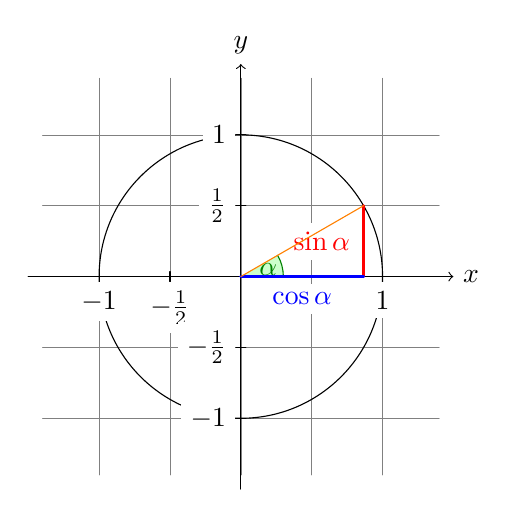
\begin{tikzpicture}
    [scale=1.8,line cap=round,
    % Styles
    axes/.style=,
    important line/.style={very thick},
    information text/.style={rounded corners,fill=red!10,inner sep=1ex}]
    % Colors
    \colorlet{anglecolor}{green!50!black}
    \colorlet{sincolor}{red}
    \colorlet{tancolor}{orange!80!black}
    \colorlet{coscolor}{blue}
    % The graphic
    \draw[help lines,step=0.5cm] (-1.4,-1.4) grid (1.4,1.4);
    \draw (0,0) circle [radius=1cm];
    \begin{scope}[axes]
      \draw[->] (-1.5,0) -- (1.5,0) node[right] {$x$} coordinate(x axis);
      \draw[->] (0,-1.5) -- (0,1.5) node[above] {$y$} coordinate(y axis);
      \foreach \x/\xtext in {-1, -.5/-\frac{1}{2}, 1}
      \draw[xshift=\x cm] (0pt,1pt) -- (0pt,-1pt) node[below,fill=white] {$\xtext$};
      \foreach \y/\ytext in {-1, -.5/-\frac{1}{2}, .5/\frac{1}{2}, 1}
      \draw[yshift=\y cm] (1pt,0pt) -- (-1pt,0pt) node[left,fill=white] {$\ytext$};
    \end{scope}
    \filldraw[fill=green!20,draw=anglecolor] (0,0) -- (3mm,0pt)
    arc [start angle=0, end angle=30, radius=3mm];
    \draw (15:2mm) node[anglecolor] {$\alpha$};
    \draw[important line,sincolor]
    (30:1cm) -- node[left=1pt,fill=white] {$\sin \alpha$} (30:1cm |- x axis);
    \draw[important line,coscolor]
    (30:1cm |- x axis) -- node[below=2pt,fill=white] {$\cos \alpha$} (0,0);
    \draw[orange] (0,0) -- (30:1cm);
  \end{tikzpicture}
  \caption{Die \textcolor{orange}{Hypotenuse} hat im Einheitskreis stets die Länge $1$. Für $\alpha = 0$ ist $\sin \alpha = 0$ und $\cos \alpha = 1$, für $\alpha = \frac{\pi}{2}$ ist $\sin \alpha = 1$ und $\cos \alpha = 0$. Dies sieht man leicht ein, indem man das entsprechende Dreieck in den Einheitskreis einzeichnet.}
\end{marginfigure}
\end{bla}

\begin{bla}{Eigenschaften von trigonometrischen Funktionen}
  \begin{itemize}
    \item \textbf{Verschiebung.} Wie jede Funktion kann auch eine trigonometrische verschoben werden. Das funktioniert genau wie bei allen bisherigen Funktionen: $f(x)=\sin(x-2)+3$ ist $\sin(x)$ um $3$ nach oben und $2$ nach rechts verschoben. Diese Operation passiert "`am nähesten"' bei $x$.
    \item \textbf{Periode.} Die Periode einer trigonometrischen Funktion ist die Länge nach der sich die Funktion wiederholt. Bei $\sin(x)$ und $\cos(x)$ ist das $2\pi$. Sie wird verändert, indem man $x$ mit einem Faktor multipliziert. Die Periode wird durch diesen Faktor \emph{geteilt}. $f(x)=\sin(3x)$ hat also die Periode $\frac{2\pi}{3}$.
    % TODO Grafik Periode
    \item \textbf{Amplitude.} Die Amplitude einer trigonometrischen Funktion ist der maximale Abstand des Graphen zur $x$-Achse. $\sin(x)$ und $\cos(x)$ haben die Amplitude $1$. Fügt man einen Faktor davor hinzu, so verändert sich die Amplitude um diesen Faktor: $f(x)=\frac{1}{2} \sin(x)$ hat die Amplitude $\frac{1}{2}$.
    % TODO Grafik Amplitude
  \end{itemize}
\end{bla}

\begin{koch}
  \textbf{Transformation an Sinus.} $f(x)=a*\sin(b(x-c))+d$ hat folgende Eigenschaften:
  \begin{itemize}
    \item Amplitude $|a|$
    \item Periode $\frac{2\pi}{b}$
    \item Verschiebung von $(0|0)$ zu $(c|d)$
  \end{itemize}
\end{koch}


\part{Analysis}
\chapter{Differentialrechnung}
\begin{inhalt}
  Bestimmen von
  \begin{itemize}
    \item Änderungsraten
    \item Ableitungen
    \item Tangenten
    \item Normalen
  \end{itemize}
\end{inhalt}

\section{Änderungsrate}

\begin{marginfigure}
  \begin{tikzpicture}[
      scale=0.5,
      thick,
      >=stealth',
      dot/.style = {
        draw,
        fill = white,
        circle,
        inner sep = 0pt,
        minimum size = 4pt
      }
    ]
    \coordinate (O) at (0,0);

    \draw[step=1cm,gray!40] (-0.1,-0.1) grid (7.9,4.9);

    % Achsen
    \draw[->] (-0.3,0) -- (8,0) coordinate[label = {below:$x$}] (xmax);
    \draw[->] (0,-0.3) -- (0,5) coordinate[label = {right:$f(x)$}] (ymax);
 
    % Pfade
    \path[name path=x] (0.3,0.5) -- (6.7,4.7);
    \path[name path=y] plot[smooth] coordinates {(-0.3,2) (2,1.5) (4,2.8) (6,5)};

    \scope[name intersections = {of = x and y, name = i}]

      % Steigungsdreieck
      \fill[gray!20] (i-1) -- (i-2 |- i-1) -- (i-2) -- cycle;

      % durchschnittliche Steigung
      \draw[black!60!green]      (0.3,0.5) -- (6.7,4.7) node[pos=0.8, below right] {};

      % Graph
      \draw[red] plot[smooth] coordinates {(-0.3,1) (2,1.5) (4,2.8) (6,5)};

      % Knoten
      \draw (i-1) node[dot, label = {}] (i-1) {} -- node[left]
        {} (i-1 |- O) node[label = {below:$x_0$}] {};
      \path (i-2) node[dot, label = {}] (i-2) {} -- (i-2 |- i-1)
        node[dot] (i-12) {};

      % y-Werte
      \draw (i-1) -- (i-1 -| 0, 0) node[thin, label = {left:$f(x_0)$}] {};
      \draw (i-2) -- (i-2 -| 0, 0) node[thin, label = {left:$f(x_0+h)$}] {};

      \draw           (i-12) -- (i-12 |- O) node[label = {below:$x_0 + h$}] {};
      \draw[blue, <->] (i-2) -- node[right] {$f(x_0 + h) - f(x_0)$}
                                (i-12);
      \draw[blue, <->] (i-1) -- node[below] {$h$} (i-12);

    \endscope
  \end{tikzpicture}
  \caption{Die \textcolor{black!60!green}{Gerade} beschreibt die Steigung des \textcolor{red}{Graphen} auf dem Intervall $[x_0,x_0+h]$.}
\end{marginfigure}

\begin{bla}{Durchschnittliche Änderungsrate}
Betrachtet man den Abschnitt einer Funktion auf einem Intervall $[x_0,x_0+h]$, so ist in diesem Intervall eine durchschnittliche Steigung feststellbar, welche durch eine Gerade durch $(x_0, f(x_0))$ und $(x_0+h, f(x_0+h))$ dargestellt werden kann. Die Steigung dieser Geraden wird \emph{durchschnittliche Änderungsrate} des Intervalls $[x_0, x_0+h]$ genannt und kann durch $\frac{f(x_0+h)-f(x_0)}{h}$ berechnet werden.
\end{bla}

\section{Ableitung}

\begin{marginfigure}
  \begin{tikzpicture}[
      scale=0.5,
      thick,
      >=stealth',
      dot/.style = {
        draw,
        fill = white,
        circle,
        inner sep = 0pt,
        minimum size = 4pt
      }
    ]
    \coordinate (O) at (0,0);

    \draw[step=1cm,gray!40] (-0.1,-0.1) grid (7.9,4.9);

    % Achsen
    \draw[->] (-0.3,0) -- (8,0) coordinate[label = {below:$x$}] (xmax);
    \draw[->] (0,-0.3) -- (0,5) coordinate[label = {right:$f(x)$}] (ymax);

    % Graph
    \draw[domain=0:5,smooth,variable=\x,red, label={right:$f$}] plot ({\x},{0.2*\x*\x});
    \draw (5,6) node[red,label= {[red]below:$f$}] {};

    % Tangente
    \draw[domain=2.2:5, variable=\x, black!60!green] plot ({\x},{1.6*(\x-4)+3.2});

    % y-Wert
    \draw (4,3.2) -- (-0.1, 3.2) node[label = {left:\quad\enspace\ $f(x_0)$}] {};

    % x-Wert und marker
    \draw (4,3.2) node[dot] {} -- (4,-0.1) node[label = {below:$x_0$}] {};
  \end{tikzpicture}
  \caption{Die Steigung der grünen Geraden ist die Ableitung von $f$ bei $x_0$. Sie ist die \textbf{Tangente} an $(x_0,f(x_0))$.}
\end{marginfigure}

\begin{bla}{Ableitung}
  \begin{marginfigure}
    \begin{tcolorbox}[colback=white!95!black,colframe=white!75!black,title=CAS:,arc=0mm]
      \begin{scriptsize}
        \textbf{Calculator}: \\*
        \menu{Menü > Analysis > Ableitung} \\*
        \hfill \( \tfrac{\partial}{\partial x}(x^2) \leadsto 2*x \)
      \end{scriptsize}
    \end{tcolorbox}
  \end{marginfigure}
  Die \emph{Ableitung} der Funktion $f$ an der Stelle $x=x_0$ ist gegeben durch den Grenzwert $\lim\limits_{h \to 0}\frac{f(x_0+h)-f(x_0)}{h}$, was bedeutet, dass wir die Länge des Intervalls, auf dem wir die Änderungsrate ermitteln, immer kleiner wird. Dieser Wert wird auch als $f'(x_0)$ bezeichnet. \\ Bildlich entspricht dieser Wert der Steigung des Graphen bei $x_0$.
\end{bla}

\clearpage

\begin{bla}{Tangente}
  \begin{marginfigure}
    \begin{tcolorbox}[colback=white!95!black,colframe=white!75!black,title=CAS:,arc=0mm]
      \begin{scriptsize}
        \textbf{Calculator}: \\*
        \menu{Menü > Analysis > Tangententerm} \\*
        \hfill \textsc{tangentLine}(\( x^2 \), \( x \), 1) \( \leadsto 2*x-1 \) \\*
        (der dritte Parameter ist der \( x \)-Wert, bei dem eine Tangente angelegt werden soll)
      \end{scriptsize}
    \end{tcolorbox}
  \end{marginfigure}
  \begin{marginfigure}
    \begin{tikzpicture}[
        scale=0.5,
        thick,
        >=stealth',
        dot/.style = {
          draw,
          fill = white,
          circle,
          inner sep = 0pt,
          minimum size = 4pt
        }
      ]
      \coordinate (O) at (0,0);

      \draw[step=1cm,gray!40] (-0.1,-0.1) grid (7.9,4.9);

      % Achsen
      \draw[->] (-0.3,0) -- (8,0) coordinate[label = {below:$x$}] (xmax);
      \draw[->] (0,-0.3) -- (0,5) coordinate[label = {right:$f(x)$}] (ymax);

      % Graph
      \draw[domain=0:5,smooth,variable=\x,red, label={right:$f$}] plot ({\x},{0.2*\x*\x});
      \draw (5,5.75) node[red,label= {[red]below:$f$}] {};

      % Konstruktion 1
      \draw[domain=-0.1:4, variable=\x, orange] plot ({\x},{\x});

      % Konstruktion 2
      \draw[domain=-0.1:3, variable=\x, brown] plot ({\x},{1.6*\x});

      % Konstruktion 3
      \draw[domain=-0.1:1.5, variable=\x, blue] plot ({\x},{1.6*\x+3.2});

      % Tangente
      \draw[domain=2.5:5, variable=\x, black!60!green] plot ({\x},{1.6*(\x-4)+3.2});

      % y-Wert
      \draw (4,3.2) -- (-0.1, 3.2) node[label = {left:$f(x_0)$}] {};

      % x-Wert und marker
      \draw (4,3.2) node[dot] {} -- (4,-0.1) node[label = {below:$x_0$}] {};
    \end{tikzpicture}
    \caption{Schritte bis zur \textcolor{black!60!green}{Tangenten}}
  \end{marginfigure}

  Die grüne Gerade im letzten Absatz ist die sogenannte \emph{Tangente} an $f$ im Punkt $(x_0, f(x_0))$. Um sie als Funktion ausdrücken zu können benötigen wir:
  \begin{itemize}
    \item die Ableitung von $f$ in $x_0$ (= $f'(x_0)$) und
    \item den Funktionswert von $f$ in $x_0$ (= $f(x_0)$).
  \end{itemize}
  Wir konstruieren die Funktion nun Stück für Stück:
  \begin{itemize}
    \item \textbf{Vorbereitung}: Die Tangente ist eine Gerade. Die einfachste Gerade ist \textcolor{orange}{$t_0(x)=x$}.
    \item \textbf{Steigung}: Die Steigung der Tangenten an $(x_0, f(x_0))$ ist $f'(x_0)$, also braucht unsere Gerade diese Steigung:\\ \textcolor{brown}{$t_1(x)=f'(x_0)*x$}
    \item \textbf{Nach oben/unten verschieben}: Wir verschieben nun die Tangente auf die richtige Höhe, nämlich $f(x_0)$: \\ \textcolor{blue}{$t_2(x)=f'(x_0)*x+f(x_0)$}
    \item \textbf{Nach links/rechts verschieben}: Nun müssen wir sie nur seitlich zu $(x_0, f(x_0))$ verschieben, indem wir in der Funktionsgleichung $x_0$ von $x$ abziehen: \\ \textcolor{black!60!green}{$t(x)=f'(x_0)*(x-x_0)+f(x_0)$} \\ Dies ist die fertige Tangente.
  \end{itemize}
  Die Gleichung von $t(x)$ oben wird auch \emph{allgemeine Tangentengleichung} genannt.
\end{bla}

\begin{bla}{Normale}
  \begin{marginfigure}[15em]
    \begin{tikzpicture}[
        scale=0.5,
        thick,
        >=stealth',
        dot/.style = {
          draw,
          fill = white,
          circle,
          inner sep = 0pt,
          minimum size = 4pt
        }
      ]
      \coordinate (O) at (0,0);

      \draw[step=1cm,gray!40] (-0.1,-0.1) grid (7.9,4.9);

      % Achsen
      \draw[->] (-0.3,0) -- (8,0) coordinate[label = {below:$x$}] (xmax);
      \draw[->] (0,-0.3) -- (0,5) coordinate[label = {right:$f(x)$}] (ymax);

      % Graph
      \draw[domain=0:5,smooth,variable=\x,red, label={right:$f$}] plot ({\x},{0.2*\x*\x});
      \draw (1,1.2) node[red,label= {[red]below:$f$}] {};

      % Tangente
      \draw[domain=2.2:5, variable=\x, black!60!green] plot ({\x},{1.6*(\x-4)+3.2});

      % Normale
      \draw[domain=2:6, variable=\x, orange] plot ({\x},{-0.625*(\x-4)+3.2});

      % y-Wert
      \draw (4,3.2) -- (-0.1, 3.2) node[label = {left:$f(x_0)$}] {};

      % x-Wert und marker
      \draw (4,3.2) node[dot] {} -- (4,-0.1) node[label = {below:$x_0$}] {};
    \end{tikzpicture}
    \caption{Tangente und Normale in $(x_0,f(x_0))$}
  \end{marginfigure}
  \begin{marginfigure}
    \begin{tcolorbox}[colback=white!95!black,colframe=white!75!black,title=CAS:,arc=0mm]
      \begin{scriptsize}
        \textbf{Calculator}: \\*
        \menu{Menü > Analysis > Normalenterm} \\*
        \hfill \textsc{normalLine}(\( x^2 \), \( x \), 1) \( \leadsto -\tfrac{1}{2}x+\tfrac{3}{2} \)
      \end{scriptsize}
    \end{tcolorbox}
  \end{marginfigure}
  Zusätzlich zur Tangente an $(x_0,f(x_0))$ kann man auch die sogenannte \emph{Normale} konstruieren. Diese steht senkrecht zur Tangente. \\
  Die Normalengleichung ist logischerweise bis auf die Steigung identisch mit der Tangentengleichung: \\
  $n(x)=-\frac{1}{f'(x_0)}*(x-x_0)+f(x_0)$
\end{bla}

\begin{koch}
  \textbf{Tangente/Normale in einem Punkt $P(x_0|f(x_0))$ bestimmen}: \\
  \begin{itemize}
    \item \textbf{Tangente}: $t(x)=f'(x_0)*(x-x_0)+f(x_0)$
    \item \textbf{Normale}: $n(x)=\frac{-1}{f'(x_0)}*(x-x_0)+f(x_0)$
  \end{itemize}
\end{koch}



\begin{bla}{Tangente durch einen Punkt anlegen}
  Gegeben ist eine Funktion (beispielsweise $f(x)=\tfrac{1}{4}*x^2$) und ein Punkt, der \emph{nicht} auf dem Graphen liegt (beispielsweisei $P(\tfrac{3}{2}|-1)$). Gesucht ist eine Tangente an $f(x)$, die durch $P$ geht.
  \begin{enumerate}
    \item Wähle beliebigen Berührpunkt von Tangente und Funktion: $B(x_0|f(x_0))$ (dieser liegt logischerweise auf der Funktion).
    \item Die Steigung der Tangenten ist
    \begin{enumerate}
      \item $f'(x_0)$
      \item Die Steigung im Steigungsdreieck: $\frac{f(x_0)-(-1)}{x_0-\tfrac{3}{2}}$
    \end{enumerate}
    \item Wir berechnen die Ableitung von $f(x)$ (wie das geht steht im nächsten Kapitel): $f'(x)=\tfrac{1}{2}*x$
    \item Wir setzen die Steigungen gleich und erhalten so $x_0$:
    \begin{equation*}
      f'(x_0)=\tfrac{1}{2}*x_0=\frac{f(x_0)-(-1)}{x_0-\tfrac{3}{2}} \Leftrightarrow {x_0}^2-3x_0-4=0
    \end{equation*}
    Mit der Mitternachtsformel erhalten wir $x_{0_1}=-1$ und $x_{0_2}=4$. Durch Einsetzen in die Funktion erhalten wir die Berührpunkte $B_1(-1|\tfrac{1}{4})$ und $B_2(4|4)$. Mit der allgemeinen Tangentengleichung erhalten wir jeweils die Tangente:
    \begin{equation*}
      t_1(x)=-\tfrac{1}{2}x- \tfrac{1}{4}
    \end{equation*}
    und
    \begin{equation*}
      t_2(x)=2x-4
    \end{equation*}
  \end{enumerate}
\end{bla}

\begin{bla}{Ableitungsfunktion}
  Wir haben oben gesehen, dass man für jedes $x_0$ die Steigung von $f$ in $x_0$ berechnen kann (bis auf Ausnahmen, aber darauf wollen wir hier noch nicht eingehen). Diese haben wir $f'(x_0)$ genannt. Wir verallgemeinern das und nennen $f'(x)$ die \emph{Ableitung} von $f$. Sie ordnet jedem $x_0$ die Steigung $f'(x_0)$ zu.
\end{bla}



\begin{bla}{Beispiel: Ableitungsfunktion berechnen}
  \begin{marginfigure}
    \begin{tikzpicture}[
        scale=0.7,
        thick,
        >=stealth',
        dot/.style = {
          draw,
          fill = white,
          circle,
          inner sep = 0pt,
          minimum size = 4pt
        }
      ]
      \coordinate (O) at (0,0);

      \draw[step=1cm,gray!40] (-2.9,-2.9) grid (2.9,2.9);

      % Achsen
      \draw[->] (-3,0) -- (3,0) coordinate[label = {below:$x$}] (xmax);
      \draw[->] (0,-3) -- (0,3) coordinate[label = {right:$f(x)$}] (ymax);

      % Graph
      \draw[domain=-2:2,smooth,variable=\x,red] plot ({\x},{\x*\x});
      \draw (2,2.5) node[red,label={[red]below:$x^2$}] {};

      % Ableitung
      \draw[domain=-1.5:2,variable=\x,black!60!green] plot ({\x},{2*\x});
      \draw (-1,-0.5) node[label={[black!60!green]below:$2x$}] {};
    \end{tikzpicture}
    \caption{$f(x)=x^2$ und $f'(x)=2x$}
  \end{marginfigure}

  Wir möchten nun die Ableitungsfunktion von $f(x)=x^2$ berechnen. Diese wird wie die Ableitung an einem Punkt berechnet: \\
  \begin{equation*}
    \begin{split}
      f'(x) & = \lim\limits_{h \to 0}\frac{f(x+h)-f(x)}{h} = \lim\limits_{h \to 0}\frac{{(x+h)}^2-x^2}{h} = \lim\limits_{h \to 0}\frac{x^2+2xh+h^2-x^2}{h} \\
      & = \lim\limits_{h \to 0}\frac{2xh+h^2}{h} = \lim\limits_{h \to 0}(2xh+h)\xrightarrow{h\rightarrow 0}2x
    \end{split}
  \end{equation*}
\end{bla}



\begin{bla}{Ableitungsregeln}
  Damit man nicht immer mühsam den Grenzwert bestimmen muss, um die Ableitungsfunktion zu erhalten, gibt es einige \emph{Ableitungsregeln} ($r$ ist eine beliebige Zahl):
  \begin{itemize}
    \item \textbf{Konstantenregel}: Die Steigung einer Konstanten ($f(x)=a$ für eine Zahl $a$) ist überall Null, also gilt für ihre Ableitung: $f'(x)=0$.
    \item \textbf{Potenzregel}: $f(x)=x^r \Rightarrow f'(x)=r*x^{r-1}$ \\
    Beispiel: $f(x)=x^2 \Rightarrow f'(x)=2*x^{2-1}=2*x$

    \item \textbf{Faktorregel}: $f(x)=r*g(x) \Rightarrow f'(x)=r*g'(x)$ \\
    Beispiel: $f(x)=2x=2x^1 \Rightarrow f'(x)=2*1*x^{1-1}=2*x^0=2*1=2$
    % TODO verstehen die das? Eventuell leichteres Beispiel ergänzen

    \item \textbf{Summenregel}: $f(x)=g(x)+h(x) \Rightarrow f'(x)=g'(x)+h'(x)$ \\
    Beispiel: $f(x)=x^2+2x \Rightarrow f'(x)=2x+2$

    \item \textbf{Produktregel}: $f(x)=g(x)*h(x) \Rightarrow f'(x)=g'(x)*h(x)+g(x)*h'(x)$ \\
    Beispiel: $f(x)=(x^2)*(2x) \Rightarrow f'(x)=(2x)*(2x)+(x^2)*(2)=4x^2+2x^2=6x^2$

    \item \textbf{Quotientenregel}: $f(x)=\frac{g(x)}{h(x)} \Rightarrow f'(x)=\frac{g'(x)*h(x)-g(x)*h'(x)}{h(x)*h(x)}$ \\
    Beispiel: $f(x)=\frac{x^2}{2x} \Rightarrow f'(x)=\frac{(2x)*(2x)-(x^2)*(2)}{(2x)*(2x)}=\frac{4x^2-2x^2}{4x^2}=\frac{2x^2}{4x^2}=\frac{1}{2}$. Das ist klar, da $\frac{x^2}{2x}=\frac{1}{2}x$.

    \item \textbf{Kettenregel}: $f(x)=g(h(x)) \Rightarrow f'(x)=g'(h(x))*h'(x)$ \\
    Beispiel: $f(x)={(2x)}^2 \Rightarrow f'(x)=(2*(2x))*(2)=4*2x=8x$ \\
    Bemerkung: Zwei Funktionen werden verkettet, indem man für jedes $x$ in der äußeren Funktion (hier also $g(x)$) die innere Funktion (hier $h(x)$) einsetzt: \\ $g(x)=x^2, h(x)=2x \rightarrow g(h(x))={(2x)}^2$
  \end{itemize}
\end{bla}



% TODO trigonometrische Funktionen erklären
\begin{bla}{Ableitungen von trigonometrischen Funktionen}
  Es gilt:
  \begin{itemize}
    \item $f(x)=\sin(x)\ \Rightarrow\  f'(x)=\cos(x)$
    \item $f(x)=\cos(x)\ \Rightarrow\ f'(x)=-\sin(x)$
  \end{itemize}
\end{bla}

\begin{bla}{Beispiel: mehrere Regeln anwenden}
  In den meisten Fällen reicht es nicht aus, nur eine Ableitungsregel zu benutzen, um die Ableitung einer Funktion zu bestimmen. Beispielsweise kann es sich um eine verkettete Funktion handeln, bei der die innere Funktion eine Summe aus zwei Funktionen ist: \\
  \begin{equation*}
    f(x)=\sqrt{2x+1}={(2x+1)}^\frac{1}{2}
  \end{equation*}
  \begin{equation*}
  \begin{split}
      f'(x) & = \frac{1}{2}*{(2x+1)}^{-\frac{1}{2}}*2 \\
      & = {(2x+1)}^{-\frac{1}{2}}  \\
      & = \frac{1}{\sqrt{2x+1}}
    \end{split}
  \end{equation*}
\end{bla}

\section{Höhere Ableitungen}
  \begin{marginfigure}
    \begin{tcolorbox}[colback=white!95!black,colframe=white!75!black,title=CAS:,arc=0mm]
      \begin{scriptsize}
        \textbf{Calculator}: \\*
        \hfill \( \tfrac{\partial}{\partial x}\left( \tfrac{\partial}{\partial x}(x^2) \right) \leadsto 2 \)
      \end{scriptsize}
    \end{tcolorbox}
  \end{marginfigure}


\begin{bla}{Höhere Ableitungen und ihre Bedeutung}
  Man kann die Ableitung einer Funktion erneut ableiten und erhält so die \emph{zweite Ableitung}, $f''(x)$.
  \begin{enumerate}
    \item \textbf{Erste Ableitung}: Die erste Ableitung stellt die Steigung der Urpsrungsfunktion dar.
    \item \textbf{Zweite Ableitung}: Die zweite Ableitung stellt die Geschwindigkeit, mit der sich die Steigung der Urpsprungsfunktion ändert, dar.
  \end{enumerate}
  \textbf{Beispiel}: $f(x)=x^2, f'(x)=2x, f''(x)=2$. Wir erkennen:
  \begin{itemize}
    \item: $2x$ ist kleiner als Null für negative $x$, also ist die Steigung von $x^2$ für $x<0$ negativ (genau gleich sieht man, dass die Steigung von $x^2$ für $x>0$ positiv ist, für $x=0$ ist die Steigung von $x^2$ Null).
    \item $f''(x)=2$ ist 2 für alle $x$, also nimmt die Steigung von $x^2$ immer zu (schaut euch dazu nochmal den Graphen von $x^2$ an!).
  \end{itemize}
\end{bla}

\begin{bla}{Links- und Rechtskurven}
  Wir haben im letzten Absatz gesehen, dass die Steigung von $x^2$ stets zunimmt (da $f''(x)=2$ immer positiv ist). Wir nennen einen Abschnitt von $f$, auf dem $f''$ positiv ist, \textbf{Linkskurve} und einen Abschnitt, auf dem $f''$ negativ ist, \textbf{Rechtskurve}.
\end{bla}

\begin{marginfigure}
  \begin{tikzpicture}[
      scale=0.7,
      thick,
      >=stealth',
      dot/.style = {
        draw,
        fill = white,
        circle,
        inner sep = 0pt,
        minimum size = 4pt
      }
    ]
    \coordinate (O) at (0,0);

    \draw[step=1cm,gray!40] (-2.9,-2.9) grid (2.9,2.9);

    % Achsen
    \draw[->] (-3,0) -- (3,0) coordinate[label = {below:$x$}] (xmax);
    \draw[->] (0,-3) -- (0,3) coordinate[label = {right:$f(x)$}] (ymax);

    % Graph Teil1
    \draw[domain=0:1.5,smooth,variable=\x,red] plot ({\x},{\x*\x*\x});

    % Graph Teil 2
    \draw[domain=-1.5:0,smooth,variable=\x,black!60!green] plot ({\x},{\x*\x*\x});

  \end{tikzpicture}
  \caption{$f(x)=x^3$ ist vor $0$ eine Rechts- und danach eine Linkskurve. Ihr könnt euch vorstellen, dass ihr von $-\infty$ nach $\infty$ auf dem Graphen entlangfahrt.}
\end{marginfigure}

\chapter{Extremstellen/-werte}
\begin{inhalt}
  Bestimmen von
  \begin{itemize}
    \item Lokalen und globalen Extrema
    \item Sattelstellen
    \item Wendestellen
    \item Lösungen von Extremwertproblemen mit Nebenbedingungen
  \end{itemize}
\end{inhalt}

Ziemlich leicht kann man Funktionen auf sogenannte \textbf{Extremstellen} untersuchen. Das sind $x$-Werte, für die die Funktion maximal bzw. minimal ist.
\begin{bla}{Lokale Extrema}
  Es gibt zwei Arten von lokalen Extrema:
  \begin{itemize}
    \item \textbf{Lokales Minimum}: Eine Funktion $f(x)$ hat bei $x_0$ dann ein lokales Minimum, wenn in einer beliebig kleinen Umgebung von $x_0$ der Funktionswert von $x_0$ der Kleinste ist.
    \item \textbf{Lokales Maximum}: Eine Funktion $f(x)$ hat bei $x_0$ dann ein lokales Maximum, wenn in einer beliebig kleinen Umgebung von $x_0$ der Funktionswert von $x_0$ der Größte ist.
  \end{itemize}

  \begin{marginfigure}[-14em]
    \begin{tikzpicture}[
        scale=1,
        thick,
        >=stealth',
        dot/.style = {
          draw,
          fill = white,
          circle,
          inner sep = 0pt,
          minimum size = 4pt
        }
      ]
      \coordinate (O) at (0,0);

      \draw[step=1cm,gray!40] (-1.9,-0.9) grid (1.9,1.9);

      % Achsen
      \draw[->] (-2,0) -- (2,0) coordinate[label = {below:$x$}] (xmax);
      \draw[->] (0,-1) -- (0,2) coordinate[label = {right:$f(x)$}] (ymax);

      % Graph
      \draw[domain=-1.5:1.2,smooth,variable=\x,red, label={right:$f$}] plot ({\x},{-\x^3+\x^2});
      \draw (1.4,-0.2) node[red,label= {[red]below:$f$}] {};

      % y-Wert
      \draw (2/3,4/27) -- (-0.1, 4/27) {};

      % x-Wert und marker
      \draw (2/3,4/27) node[dot] {} -- (2/3,-0.1) node[label = {below:\footnotesize $\tfrac{2}{3}$}] {};
    \end{tikzpicture}
    \caption{$f(x)=-x^3+x^2$ hat bei $\frac{2}{3}$ ein lokales Maximum, aber \textbf{kein} globales!}
  \end{marginfigure}
\end{bla}

\begin{bla}{globale Extrema}
  \begin{marginfigure}
    \begin{tcolorbox}[colback=white!95!black,colframe=white!75!black,title=CAS:,arc=0mm]
      \begin{scriptsize}
        \textbf{Calculator}: \\*
        \menu{Menü > Analysis > Funktionsmaximum} \\*
          \hfill \textsc{fMax}(\( x^2 \)) \( \leadsto 0 \) \\* \ \\*
        \textbf{Graph}: \\*
        \menu{Menü > Graph anal. > Maximum > Schranken wählen}
      \end{scriptsize}
    \end{tcolorbox}
  \end{marginfigure}
  Spezielle Maxima sind die sogenannten \emph{globalen Extrema}.
  \begin{itemize}
    \item \textbf{Globales Minimum}: Hat $f(x)$ in $x_{\min}$ ein lokales Minimum und gibt es keine anderen Werte für $x$, die einen kleineren Funktionswert haben, so hat $f(x)$ in $x_0$ ein \emph{globales Minimum}.
    \item \textbf{Globales Maximum}: Hat $f(x)$ in $x_{\max}$ ein lokales Maximum und gibt es keine anderen Werte für $x$, die einen größeren Funktionswert haben, so hat $f(x)$ in $x_0$ ein \emph{globales Maximum}.
  \end{itemize}
\end{bla}

\begin{bla}{Beispiel: globale Extrema}
  $f_1(x)=x^2+1$ hat in $x_0=0$ ein globales Minimum, \\ $f_2(x)=-x^2-1$ hat in $x_0=0$ ein globales Maximum. Malt euch die Graphen auf, falls ihr sie euch nicht vorstellen könnt.
\end{bla}

\begin{bla}{Hoch- und Tiefpunkte}
  In den letzten Absätzen haben wir uns mit lokalen und globalen Extremstellen beschäftigt. Mit \emph{Extrem\textbf{stellen}} war dort stets der jeweilige $x$-Wert gemeint. Möchte man von dem Punkt sprechen, bei dem der Graph maximal beziehungsweise minimal ist, so sagt man:
  \begin{itemize}
    \item \textbf{Tiefpunkt}: Hat $f(x)$ in $x_{\min}$ ein lokales Minimum, so ist $T=(x_{\min},f(x_{\min}))$ ein \emph{Tiefpunkt} von $f$.
    \item \textbf{Hochpunkt}: Hat $f(x)$ in $x_{\max}$ ein lokales Maximum, so ist $H=(x_{\max},f(x_{\max}))$ ein \emph{Hochpunkt} von $f$.
  \end{itemize}
  \textcolor{red!75!black}{\textbf{Achtung!}} Hier besteht sehr große Verwechslungsgefahr! Achtet in Aufgabenstellungen immer sehr genau darauf, was von euch verlangt wird.
\end{bla}

\begin{bla}{Vorzeichenwechsel}
  Um im nächsten Absatz die Bedingungen für Extrema beschreiben zu können müssen wir wissen, was ein Vorzeichenwechsel ist. \\ Ein \emph{Vorzeichenwechsel} liegt an einer Stelle vor, an der der Graph der Funktion die $x$-Achse schneidet. Ein Vorzeichenwechsel kann entweder von $-$ nach $+$ oder von $+$ nach $-$ erfolgen.
\end{bla}

\begin{bla}{Bedingungen für Extrema}
  In $x_0$ kann nur eine Extremstelle vorliegen wenn $f'(x_0)=0$. Oder anders formuliert:
  \begin{itemize}
    \item \textbf{Notwendige Bedingung}: Hat $f$ in $x_0$ eine Extremstelle, so ist $f'(x_0)=0$. \\
    Hinweis: Das bedeutet, dass es $x_{\text{fake}}$ geben kann, sodass $f'(x_{fake})=0$ aber $f$ keine Extremstelle in $x_{\text{fake}}$ hat! Dies ist beispielsweise in Sattelpunkten der Fall.
  \end{itemize}
  Wir brauchen also noch eine Bedingung. Diese ist die
  \begin{itemize}
    \item \textbf{Erste hinreichende Bedingung}: Ist die notwendige Bedingung erfüllt und hat $f'$ bei $x_0$ einen Vorzeichenwechsel von $-$ nach $+$, so hat $f$ in $x_0$ ein lokales Minimum (bei einem Maximum liegt ein Vorzeichenwechsel von $+$ nach $-$ vor).
  \end{itemize}
  Oft einfacher zu vernwenden ist die
  \begin{itemize}
    \item \textbf{Zweite hinreichende Bedingung}: Ist die notwendige Bedingung erfüllt und \\ $f''(x_0)<0$, liegt also $x_0$ in einer Rechtskurve, so hat $f$ in $x_0$ ein lokales Maximum (lokales Minimum für $f''(x_0)>0$ (Linkskurve)).
  \end{itemize}
\end{bla}

\begin{bla}{Sattelstellen/-punkte}
  Ist für ein $x_0$ die notwendige Bedingung erfüllt, aber keine der beiden hinreichenden, so liegt eine Sattelstelle vor. Das bedeutet, dass $f'(x_0)=0$, aber kein Vorzeichenwechsel vorliegt. \\ Der Punkt $(x_0,f(x_0))$ ist dann ein \emph{Sattelpunkt} von $f$.
\end{bla}

\begin{marginfigure}
  \begin{tikzpicture}[
      scale=0.7,
      thick,
      >=stealth',
      dot/.style = {
        draw,
        fill = white,
        circle,
        inner sep = 0pt,
        minimum size = 4pt
      }
    ]
    \coordinate (O) at (0,0);

    \draw[step=1cm,gray!40] (-2.9,-2.9) grid (2.9,2.9);

    % Achsen
    \draw[->] (-3,0) -- (3,0) coordinate[label = {below:$x$}] (xmax);
    \draw[->] (0,-3) -- (0,3) coordinate[label = {right:$f(x)$}] (ymax);

    % Graph
    \draw[domain=-0.5:2,smooth,variable=\x,red] plot ({\x},{(\x-1)^3+1});
    \draw (2.1,2.1) node[red,label= {[red]below:$f$}] {};

    % y-Wert
    \draw (1,1) -- (-0.1, 1) node[label = {left:\footnotesize $1$}] {};

    % x-Wert und marker
    \draw (1,1) node[dot] {} -- (1,-0.1) node[label = {below:\footnotesize $1$}] {};

    % Tangente
    \draw[dashed,gray] (-2,1) -- (2.8,1);
  \end{tikzpicture}
  \caption{$f(x)={(x-1)}^3+1$ hat in $x_{\text{Sattel}}=1$ eine Sattelstelle.}
\end{marginfigure}

\begin{bla}{Wendestellen/-punkte}
  \begin{marginfigure}
    \begin{tcolorbox}[colback=white!95!black,colframe=white!75!black,title=CAS:,arc=0mm]
      \begin{scriptsize}
        \textbf{Graph}: \\*
        \menu{Menü > Graph anal. > Wendepunkt > Schranken wählen} 
      \end{scriptsize}
    \end{tcolorbox}
  \end{marginfigure}

  \begin{marginfigure}
    \begin{tikzpicture}[
        scale=0.7,
        thick,
        >=stealth',
        dot/.style = {
          draw,
          fill = white,
          circle,
          inner sep = 0pt,
          minimum size = 4pt
        }
      ]
      \coordinate (O) at (0,0);

      \draw[step=1cm,gray!40] (-4.4,-1.9) grid (4.4,1.9);

      % Achsen
      \draw[->] (-4.5,0) -- (4.5,0) coordinate[label = {below:$x$}] (xmax);
      \draw[->] (0,-2) -- (0,2) coordinate[label = {right:$f(x)$}] (ymax);

      % Graph
      \draw[domain=-4:4,smooth,variable=\x,red, label={right:$f$}] plot ({\x},{sin(deg(\x))});
      \draw (3.141592-0.5,1.3) node[red,label= {[red]below:$f$}] {};

      % Tangente
      \draw[dashed,gray] (-2,-2) -- (2,2);

      % Ursprung
      \draw (0,0) node[dot] {};
    \end{tikzpicture}
    \caption{$f(x)=\sin(x)$ hat in $x_{\text{Wende}}=0$ eine Wendestelle. Wenn man auf dem Graph von $-\infty$ nach $\infty$ fahren würde, so stünde hier das Lenkrad gerade.}
  \end{marginfigure}

  Die Stellen, an denen eine Funktion $f$ von einer Links- in eine Rechtskurve wechselt --- oder umgekehrt --- nennt man \emph{Wendestellen}. Die Bedingungen sind sehr ähnlich wie die Bedingungen für Extrema und sind graphisch leicht nachvollziehbar:
  \begin{itemize}
    \item \textbf{Notwendige Bedingung}: $f$ kann in $x_0$ nur dann eine Wendestelle haben, wenn $f''(x_0)=0$ gilt (da $f''(x_0) < 0$ für eine Rechts- und $f''(x_0) > 0$ für eine Linkskurve).
    \item \textbf{Erste hinreichende Bedingung}: Ist die notwendige Bedingung erfüllt und hat $f''$ in $x_0$ einen Vorzeichenwechsel, so hat $f$ in $x_0$ eine Wendestelle.
    \item \textbf{Zweite hinreichende Bedingung}: Ist die notwendige Bedingung erfüllt und ist $f'''(x_0)\neq 0$, so hat $f$ in $x_0$ eine Wendestelle.
  \end{itemize}
  Wie bei den Extrema definiert man für eine Wendestelle von $f$ bei $x_0$ den zugehörigen Wendepunkt $(x_0,f(x_0))$.
\end{bla}

\section{Extremwertprobleme mit Nebenbedingungen}

\begin{bla}{Beispiel: Fläche maximieren}
  \begin{marginfigure}[5em]
    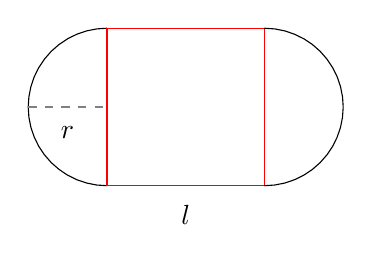
\begin{tikzpicture}
      % Laufbahn und Feld
      \draw [domain=270:90] plot ({cos(\x)}, {sin(\x)});
      \draw [domain=0:2,red] plot ({\x},{1});
      \draw [domain=0:2,red] plot ({\x},{-1});
      \draw [domain=-1:0,gray,dashed] plot ({\x},{0});
      \draw [domain=-1:1,red,variable=\y] plot ({0},{\y});
      \draw [domain=-1:1,red,variable=\y] plot ({2},{\y});
      \draw [domain=-90:90] plot ({cos(\x)+2}, {sin(\x)});

      % Beschriftung
      \draw (1,-1) node[label={below:$l$}] {};
      \draw (-0.5,0) node[label={below:$r$}] {};
    \end{tikzpicture}
    \caption{Das \textcolor{red}{Spielfeld} soll möglichst groß werden. Wie müssen $l$ und $r$ gewählt werden?}
  \end{marginfigure}
  Eine 400m-Laufbahn soll so gemacht werden, dass das rechteckige Spielfeld in der Mitte der Laufbahn möglichst groß wird. Wie sind $l$ und $r$ zu wählen, damit diese Fläche maximal wird?
\end{bla}

\begin{koch}
  \textbf{Lösungsstrategie für Extremwertprobleme mit Nebenbedingungen}:
  \begin{enumerate}
    \item Die Größe, die maximal/minimal werden soll, durch einen Term beschreiben.
    \item Bedingung in den Term einsetzen $\rightarrow$ Größe hängt nur noch von einer Variablen ab
    \item Term ableiten und Nullstellen bestimmen $\rightarrow$ Minima/Maxima der Größe
    \item Testen: Sind die Ergebnisse sinnvoll?
  \end{enumerate}
\end{koch}



\begin{bla}{Lösung des Beispiels}
  Wir lösen das Beispiel mit dem Kochrezept.
  \begin{enumerate}
    \item Die Fläche des Rechtecks wird beschrieben durch $A_{l,r}=l*2r$.
    \item Die Bedingung ist $400=2l+2\pi r$. Um die Bedingung in den obigen Term einsetzen zu können formen wir die Bedingung nach einer Variable um, beispielsweise nach $l$: $l=200-\pi r$. Wir erhalten also durch Einsetzen: $A(r)=(200-\pi r)*2r=400r-2\pi r^2$.
    \item Die Ableitung von $A(r)$ ist $A'(r)=400-4\pi r$. Als Nullstellen erhalten wir:
    \begin{equation*}
      A'(r)=0 \Leftrightarrow 400-4\pi r = 0 \Leftrightarrow 100=\pi r \Leftrightarrow r = \tfrac{100}{\pi}
    \end{equation*}
    Die beiden Kreisbögen haben also zusammen die Länge $2\pi r = 2\pi \tfrac{100}{\pi} = 200m$. Also ist $l=100m$.
    \item Wir müssen das Ergebnis nicht testen, tatsächlich ist die gerade Strecke bei einer echten $400m$-Laufbahn $100m$ lang.
  \end{enumerate}
\end{bla}

\chapter{Exponentialfunktionen}
\begin{inhalt}
  \begin{itemize}
    \item Eulersche Zahl
    \item Exponentialfunktion und Logarithmus
  \end{itemize}
\end{inhalt}

\begin{bla}{Eulersche Zahl, natürliche Exponentialfunktion}
  Leitet man eine Exponentialfunktion der Form $f(x)=a^x$ mit dem Taschenrechner ab, so sieht man, dass es ein $n$ gibt, sodass $f'(x)=n*f(x)$.
  Wir suchen nun $e$ derart, dass die Ableitung von $e^x$ wieder $e^x$ ist (also $n=1$).
  Diese Zahl heißt \emph{eulersche Zahl}. Es gilt:
  \begin{equation*}
    f(x)=e^x \rightsquigarrow f'(x)=f(x)
  \end{equation*}
  Wir nennen diese Funktion auch \emph{natürliche Exponentialfunktion}.
\end{bla}

\begin{bla}{Natürlicher Logarithmus}
  Der \emph{natürliche Logarithmus} ist die Gegenfunktion zur natürlichen
  Exponentialfunktion. Da sie die Gegenfunktion ist gilt:
  \begin{itemize}
    \item $\ln(e^x)=x$
    \item $e^{\ln(x)}=x$
  \end{itemize}
\end{bla}

\begin{marginfigure}
  \begin{tikzpicture}[
      scale=0.7,
      thick,
      >=stealth',
      dot/.style = {
        draw,
        fill = white,
        circle,
        inner sep = 0pt,
        minimum size = 4pt
      }
    ]
    \coordinate (O) at (0,0);

    \draw[step=1cm,gray!40] (-3.9,-3.9) grid (3.9,3.9);

    % Achsen
    \draw[->] (-4,0) -- (4,0) coordinate[label = {below:$x$}] (xmax);
    \draw[->] (0,-4) -- (0,4) coordinate[label = {right:$f(x)$}] (ymax);

    % Graph e^x
    \draw[domain=-3:1.5,smooth,variable=\x,red, label={right:$f$}] plot ({\x},{exp(\x)});
    \draw (2,4.5) node[red,label= {[red]below:$e^x$}] {};

    % Graph ln(x)
    \draw[domain=0.05:4,smooth,variable=\x,black!60!green] plot ({\x},{ln(\x)});
    \draw (3,1) node[red,label= {[black!60!green]below:$ln(x)$}] {};


    % Spiegelung
    \draw[dashed,gray] (-2,-2) -- (2,2);
    \draw (2,2) node[label= {[gray]right:Spiegelung}] {};
  \end{tikzpicture}
  \caption{$e^x$ und $\ln(x)$.}
\end{marginfigure}

\begin{bla}{Logarithmus und Exponentialfunktion: Wichtige Punkte}
  Ein paar wichtige Werte von $e^x$ und $\ln(x)$ sollte man sich merken, da so später Gleichungen oft stark vereinfacht werden können ($f(x)=e^x, g(x)=\ln(x)$):
  \begin{itemize}
    \item $f(0)=e^0=1$
    \item $f(1)=e^1=e$
    \item $g(x)=\ln(x)$ ist nur für positive $x$ definiert
    \item $g(1)=\ln(1)=0$
    \item $g(e)=\ln(e)=1$
  \end{itemize}
\end{bla}

\begin{bla}{Rechenregeln}
  Mit diesen Regeln lassen sich Exponentialgleichungen lösen. Diese Regeln wurden bereits im Grundlagenkapitel erwähnt.
  \begin{itemize}
    \item $\ln(u*v)=\ln(u)+\ln(v)$
    \item $\ln(\frac{u}{v})=\ln(u)-\ln(v)$
    \item $\ln(a^k)=k*\ln(a) \rightsquigarrow a^k=e^{k*\ln(a)}$
    \item $f(x)=a^x \rightsquigarrow f'(x)=\ln(a)*a^x$ (folgt aus der Kettenregel)
  \end{itemize}
\end{bla}

\begin{bla}{Beispiele zum Lösen von Exponential- und Logarithmusgleichungen} \  \\
  Es gibt verschiedene Ansätze um Exponential- und Logarithmusgleichungen zu lösen:
  \begin{enumerate}
    \item \textbf{Naives Umformen}: Sehr einfache Terme können durch naives Umformen gelöst werden:
      \begin{alignat*}{3}
        & e^x-e^{2x}=0\  && |+e^{2x} \\
        \Leftrightarrow\  & e^x=e^{2x} && |\ln \\
        \Leftrightarrow\  & x=2x && \\
        \rightsquigarrow & x=0 &&
      \end{alignat*}
    \item \textbf{Nullprodukt}: Ein Produkt von zwei Termen wird genau dann Null, wenn einer der beiden Terme Null ist:
      \begin{alignat*}{3}
        & (x-1)*(e^x-1)=0 && | \text{\ Terme einzeln betrachten} \\
        \Leftrightarrow\  & (x-1)=0 \text{\ oder\ } e^x-1=0 && \\
        \Leftrightarrow\  & x=1 \text{\ oder\ } e^x=1 && \\
        \Leftrightarrow\ & x=1 \text{\ oder\ } x=0 && \\
      \end{alignat*}
    \item \textbf{Substitution}: Die Substitution funktioniert auch hier:
      \begin{alignat*}{3}
        & e^x-3e^{-x}+2=0 && | *e^x\\
        \Leftrightarrow\  & e^{2x}-3+2e^x=0 && |\  \text{Substitiution:\ } u=e^x \\
        \Leftrightarrow\  & u^2+2u-3=0 && |\  \text{Mitternachtsformel} \\
        \rightsquigarrow\  & u_1=1, u_2=-\frac{3}{2} && |\ \text{Rücksubstitution} \\
        \Leftrightarrow\ & 1=e^{x_1}, -\frac{3}{2}=e^{x_2} && |\ \ln \\
        \Leftrightarrow\ & x_1=\ln(1), x_2=\ln(-\frac{3}{2}) \\
        \rightsquigarrow\ & x=x_1=\ln(1)=0 &&
      \end{alignat*}
      Das Ergebnis $x_2$ gibt es nicht, da $\ln(x)$ nur für positive $x$ definiert ist.
  \end{enumerate}
\end{bla}

\chapter{Funktionenscharen}
\begin{inhalt}
  \begin{itemize}
    \item Funktionenscharen
    \item Extremstellen von Funktionenscharen
    \item Ortslinien
  \end{itemize}
\end{inhalt}

\begin{bla}{Funktionenschar}
  \begin{marginfigure}[4em]
    \begin{tcolorbox}[colback=white!95!black,colframe=white!75!black,title=CAS:,arc=0mm]
      \begin{scriptsize}
        \textbf{Graph}: \\*
        \hfill \( f1(x) = \{ 1, 2, 3 \}x^2 \) \\*
        \( \leadsto \) Graphen von \( x^2 \), \( 2x^2 \) und \( 3x^2 \)
      \end{scriptsize}
    \end{tcolorbox}
  \end{marginfigure}
  Eine \emph{Funktionenschar} ist eine Funktion, die zusätzlich zu $x$ noch einen weiteren Parameter $k$ enthält (man schreibt $f_k(x)$). Setzt man für $k$ einen Wert ein, so erhält man eine Funktion aus der unendlich großen Funktionenschar.
\end{bla}

\begin{bla}{Beispiel: eine Funktionenschar}
  Wir betrachten die Funktionenschar $f_k(x)=\frac{1}{k}*x^2$. Wir setzen ein paar Werte für $k$ ein:
  \begin{itemize}
    \item $f_1(x)=x^2$
    \item $f_{-2}(x)=-\frac{1}{2}*x^2$
    \item $f_3(x)=\frac{1}{3}*x^2$
  \end{itemize}

  \begin{marginfigure}
    \begin{tikzpicture}[
        scale=0.7,
        thick,
        >=stealth',
        dot/.style = {
          draw,
          fill = white,
          circle,
          inner sep = 0pt,
          minimum size = 4pt
        }
      ]
      \coordinate (O) at (0,0);

      \draw[step=1cm,gray!40] (-2.9,-2.9) grid (2.9,2.9);

      % Achsen
      \draw[->] (-3,0) -- (3,0) coordinate[label = {below:$x$}] (xmax);
      \draw[->] (0,-3) -- (0,3) coordinate[label = {right:$f(x)$}] (ymax);

      % Graph f_1
      \draw[domain=-2:2,smooth,variable=\x,red, label={right:$f$}] plot ({\x},{\x*\x});
      \draw (2,3.5) node[red,label= {[red]below:$f_1$}] {};

      % Graph f_{-2}
      \draw[domain=-2:2,smooth,variable=\x,orange, label={right:$f$}] plot ({\x},{-0.5*\x*\x});
      \draw (2,-0.8) node[red,label= {[orange]below:$f_{-2}$}] {};

      % Graph f_3
      \draw[domain=-2:2,smooth,variable=\x,blue, label={right:$f$}] plot ({\x},{0.33333*\x*\x});
      \draw (2,1.2) node[red,label= {[blue]below:$f_3$}] {};
    \end{tikzpicture}
    \caption{Graphen der drei Funktionen aus der Funktionenschar}
  \end{marginfigure}
\end{bla}

\begin{bla}{Bemerkung: Spiegelung an der $x$-Achse}
  Wählt man für $k$ eine negative Zahl, so ergibt sich oft ein ganz anderer Verlauf der Funktion als für ein positives $k$. Ist dies der Fall, so müssen wir die Funktionenschar für positive und negative $k$ getrennt betrachten.
\end{bla}



\begin{bla}{Untersuchung einer Funktionenschar auf Extremstellen} \  \\
  Wie eine Funktion kann auch eine Funktionenschar auf die üblichen Punkte und Stellen untersucht werden. Dabei wird $k$ einfach wie eine ganz normale Zahl behandelt. Man erhält also die Extremstellen/-punkte in Abhängigkeit von $k$.
\end{bla}

\begin{bla}{Beispiel: Untersuchung einer Funktionenschar auf Extrempunkte} \  \\
  Wir betrachten die Funktionenschar $f_k(x)=k*x^2$. Wir sehen, dass für negative $k$ eine Spiegelung an der $x$-Achse auftritt. Wir betrachten also positive und negative $k$ getrennt.
  \begin{itemize}
    \item \textbf{Fall 1}: $k>0$. Es ist $f'_k(x)=2kx$. Wir betrachten die Nullstellen der Ableitung: \\
    $f'_k(x)=0\  \Leftrightarrow\  2kx=0\  \Leftrightarrow\  x=0$. Also hat $f_k(x)$ für $x=0$ ein Extremum. \\
    Die zweite Ableitung ist $f''_k(x)=2k$. Da $k>0$ ist, ist $f''_k(0)=2k>0$, also hat $f_k(x)$ für $k>0$ in $x=0$ ein Minimum.

    \item \textbf{Fall 2}: $k<0$. Es ist $f'_k(x)=2kx$. Auch hier erhalten wir als Nullstelle der Ableitung $x=0$. \\
    Die zweite Ableitung ist $f''_k(x)=2k$. Da $k<0$ ist, ist $f''_k(0)=2k<0$, also hat $f_k(x)$ für $k<0$ in $x=0$ ein Maximum.
  \end{itemize}

  \begin{marginfigure}[-25em]
    \begin{tikzpicture}[
        thick,
        >=stealth',
        dot/.style = {
          draw,
          fill = white,
          circle,
          inner sep = 0pt,
          minimum size = 4pt
        }
      ]
      \coordinate (O) at (0,0);

      \draw[step=1cm,gray!40] (-2.9,-2.9) grid (2.9,2.9);

      % Achsen
      \draw[->] (-3,0) -- (3,0) coordinate[label = {below:$x$}] (xmax);
      \draw[->] (0,-3) -- (0,3) coordinate[label = {right:$f(x)$}] (ymax);

      % Graph f_k<0
      \draw[domain=-2:2,smooth,variable=\x,red, label={right:$f$}] plot ({\x},{-0.2*\x*\x});
      \draw[domain=-2:2,smooth,variable=\x,red, label={right:$f$}] plot ({\x},{-0.5*\x*\x});
      \draw[domain=-1.5:1.5,smooth,variable=\x,red, label={right:$f$}] plot ({\x},{-\x*\x});

      % Graph f_k>0
      \draw[domain=-2:2,smooth,variable=\x,black!60!green, label={right:$f$}] plot ({\x},{0.2*\x*\x});
      \draw[domain=-2:2,smooth,variable=\x,black!60!green, label={right:$f$}] plot ({\x},{0.5*\x*\x});
      \draw[domain=-1.5:1.5,smooth,variable=\x,black!60!green, label={right:$f$}] plot ({\x},{\x*\x});

      % Ursprung
      \draw (0,0) node[dot] {};
    \end{tikzpicture}
    \caption{Fallunterscheidung für positive und negative $k$}
  \end{marginfigure}
\end{bla}

\begin{bla}{Ortslinien}
  Wir haben im letzten Beispiel gesehen, dass man Extrema von Funktionenscharen im Abhängigkeit von $k$ erhalten kann. Ist das so, so kann man eine Funktion aufstellen, die durch diese Extrema verläuft. Das ist die sogenannte \emph{Ortslinie} des Extremums.
\end{bla}

\begin{bla}{Berechnung der Ortslinie}
  Wir werden jetzt die Ortslinie aus obiger Grafik berechnen. \\
  Die betrachtete Funktionenschar ist $f_k(x)={(x-k)}^2+k$. Es ist $f'_k(x)=2(x-k)$. \\
  $f'_k(x)=0\  \Leftrightarrow\  2(x-k)=0\  \Leftrightarrow\  x-k=0\  \Leftrightarrow\  x=k$.\\
  Das bedeutet, dass $f_k(x)$ für $x=k$ ein Extremum hat. Der $y$-Wert für $x=k$ ist \\
  $f_k(k)={(k-k)}^2+k=k$. Die Extrema liegen also auf $o(k)=k$. \\
  Dies ist die Ortslinie der Extrema.

  \begin{marginfigure}[-10em]
    \begin{tikzpicture}[
        scale=0.7,
        thick,
        >=stealth',
        dot/.style = {
          draw,
          fill = white,
          circle,
          inner sep = 0pt,
          minimum size = 4pt
        }
      ]
      \coordinate (O) at (0,0);

      \draw[step=1cm,gray!40] (-1.9,-0.1) grid (3.9,5.9);

      % Achsen
      \draw[->] (-2,0) -- (4,0) coordinate[label = {below:$x$}] (xmax);
      \draw[->] (0,-0.1) -- (0,6) coordinate[label = {right:$f(x)$}] (ymax);

      % Graphen
      \draw[domain=-2:2,smooth,variable=\x,gray, label={right:$f$}] plot ({\x},{(\x)^2});
      \draw[domain=-1:3,smooth,variable=\x,gray, label={right:$f$}] plot ({\x},{(\x-1)^2+1});
      \draw[domain=0:4,smooth,variable=\x,gray, label={right:$f$}] plot ({\x},{(\x-2)^2+2});

      % Ortslinie
      \draw[dashed, red] (-0.3,-0.3) -- (3.5,3.5);


      % Extrema
      \draw (0,0) node[dot] {};
      \draw (1,1) node[dot] {};
      \draw (2,2) node[dot] {};

    \end{tikzpicture}
    \caption{Ein paar Funktionen und die Ortslinie von $f_k(x)={(x-k)}^2+k$.}
  \end{marginfigure}
\end{bla}

\begin{bla}{Gemeinsame Punkte}
  In Abbildung 7.2 haben alle Funktionen der Funktionenschar einen gemeinsamen Punkt ($P(0|0)$).
  Möchte man die gemeinsamen Punkte von zwei Funktionen der Funktionenschar bestimmen, so geht man so vor:
  \begin{enumerate}
    \item Wir nehmen $t_1 \neq t_2$ und stellen für diese beiden Variablen die zugehörigen Funktionen der Funktionenschar auf, also $f_{t_1}(x)$ und $f_{t_2}(x)$.
    \item Wir setzen die beiden Funktionen gleich: $f_{t_1}(x)=f_{t_2}(x)$
    \item Wir lösen die Gleichung für $x$.
    item Wir setzen die erhaltenen $x$-Werte (sie hängen in der Regel von $t_1$ und $t_2$ ab) in die Gleichung der Funktionenschar ein und erhalten so die gemeinsamen Punkte von $f_{t_1}(x)$ und $f_{t_2}(x)$. 
  \end{enumerate}
\end{bla}

\chapter{Integralrechnung}
\begin{inhalt}
  \begin{itemize}
    \item Stammfunktionen und Integrale
    \item Integrale bestimmen: Annäherung und Hauptsatz
    \item Uneigentliche Integrale
    \item Mittelwert
    \item Von Graphen beschränkte Flächen und Rotationskörper
  \end{itemize}
\end{inhalt}

In diesem Kapitel werden wir uns mit der sogenannten \emph{Integralrechnung} beschäftigen. Ein wichtiges Hilfsmittel wird sein, Funktionen nicht nur ab-, sondern auch \textbf{aufleiten} zu können. Diese Aufleitungen nennen wir \emph{Stammfunktionen}.

\section{Stammfunktionen}

\begin{bla}{Stammfunktion}
  \begin{marginfigure}
    \begin{tcolorbox}[colback=white!95!black,colframe=white!75!black,title=CAS:,arc=0mm]
      \begin{scriptsize}
        \textbf{Calculator}: \\*
        \menu{Menü > Analysis > Integral} \\*
        \hfill \( \int_{\Box}^{\Box}x^2 dx \leadsto \tfrac{x^3}{3} \)
      \end{scriptsize}
    \end{tcolorbox}
  \end{marginfigure}
  Eine Stammfunktion $F$ zu einer gegebenen Funktion $f$ ist eine Funktion, sodass $F'(x)=f(x)$ gilt. $f$ ist also die Ableitung von $F$. Um eine Stammfunktion zu $f$ zu konstruieren, müssen wir $f$ aufleiten.
\end{bla}

\begin{bla}{Aufleitungsregeln}
  Das Aufleiten funktioniert genau wie das Ableiten, nur rückwärts. Zur Vereinfachung gibt es ein paar Regeln:
  \begin{itemize}
    \item \textbf{Potenzregel}: $f(x)=x^r\ \Rightarrow\ F(x)=\frac{1}{n+1}x^{n+1}$.\\
    Dass diese Regel gilt sieht man leicht ein, indem man $F$ ableitet und $f$ erhält (dies gilt auch für alle anderen Regeln).

    \item \textbf{Summenregel}: $f(x)=g(x)+h(x)\ \Rightarrow\ F(x)=G(x)+H(x)$

    \item \textbf{Faktorregel}: $f(x)=c*g(x)\  \Rightarrow\  F(x)=c*G(x)$

    \item \textbf{Kettenregel}: $f(x)=g(cx+d)\ \Rightarrow\ F(x)=\frac{1}{c}G(cx+d)$ ($c$ und $d$ sind Zahlen).
  \end{itemize}
\end{bla}

\begin{bla}{Stammfunktionen zu speziellen Funktionen}
  Viele Funktionen können mit den vier Regeln nicht aufgeleitet werden. Es gibt aber noch einige Funktionen, deren Stammfunktionen man kennen sollte:
  \begin{itemize}
    \item $f(x)=\frac{1}{x}\ \Rightarrow\  F(x)=\ln(x)$

    \item $f(x)=a^x\  \Rightarrow\  F(x)=\frac{a^x}{\ln(a)}$

    \item $f(x)=\sin(x)\  \Rightarrow\  F(x)=-\cos(x)$

    \item $f(x)=\cos(x)\  \Rightarrow\  F(x)=\sin(x)$
  \end{itemize}
  Man sieht diese Regeln leicht ein, in dem man die Ableitungen der Stammfunktionen bildet.
\end{bla}

\section{Integrale}

\begin{bla}{Orientierter Flächeninhalt}
  Wir werden im Folgenden den Flächeninhalt zwischen einem Funktionsgraphen und der $x$-Achse betrachten. Es gilt zu beachten, dass hierbei der Flächeninhalt unterhalb der $x$-Achse als negativ betrachtet wird.
\end{bla}

\begin{marginfigure}
  \begin{tikzpicture}[
      scale=0.7,
      thick,
      >=stealth',
      dot/.style = {
        draw,
        fill = white,
        circle,
        inner sep = 0pt,
        minimum size = 4pt
      }
    ]
    \coordinate (O) at (0,0);

    \draw[step=1cm,gray!40] (-3.9,-1.4) grid (3.9,1.4);

    % Flächeninhalt oberhalb
    \fill[green!30,domain=0:3.141592] (0,0) -- plot({\x},{sin(deg(\x))}) -- (3.141592,0) -- cycle;

    % Flächeninhalt unterhalb
    \fill[red!20,domain=-3.141592:0] (-3.141592,0) -- plot({\x},{sin(deg(\x))}) -- (0,0) -- cycle;

    % Achsen
    \draw[->] (-4,0) -- (4,0) coordinate[label = {below:$x$}] (xmax);
    \draw[->] (0,-1.5) -- (0,1.5) coordinate[label = {right:$f(x)$}] (ymax);

    % Graph
    \draw[domain=-3.8:3.8,smooth,variable=\x,red] plot ({\x},{sin(deg(\x))});
    \draw (3.4,1) node[red,label={[red]below:$sin(x)$}] {};

    % Nullstellen
    \draw[-] (-3.141592,-0.1) -- (-3.141592,0.1) node[label={above:$-\pi$}] {};
    \draw[-] (3.141592,-0.1) -- (3.141592,0.1) node[label={below:$\pi$}] {};
  \end{tikzpicture}
  \caption{\textcolor{red}{Negativer} und \textcolor{black!20!green}{positiver} Flächeninhalt von $f(x)=\sin(x)$ auf $[-\pi,\pi]$. Die Summe des Flächeninhaltes der beiden Flächen beträgt Null!}
\end{marginfigure}

\begin{bla}{Bemerkung: Berechnung der Fläche unter einer Kurve durch Approximation}
  Anschaulich kann man den Flächeninhalt unter einer Kurve berechnen, indem man Rechtecke unter die Kurve zeichnet. Macht man diese Rechtecke immer dünner, so wird die Annäherung immer genauer.

  \begin{marginfigure}
    \begin{tikzpicture}[
        scale=0.7,
        thick,
        >=stealth',
        dot/.style = {
          draw,
          fill = white,
          circle,
          inner sep = 0pt,
          minimum size = 4pt
        }
      ]
      \coordinate (O) at (0,0);

      \draw[step=1cm,gray!40] (-0.1,-0.1) grid (5.9,2.9);

      % Rechteck 1
      \draw[-,black!60!green] (0,0) -- (1,0) -- (1,0.7071) -- (0,0.7071) -- cycle;
      \fill[green!30] (0,0) -- (1,0) -- (1,0.7071) -- (0,0.7071) -- cycle;

      % Rechteck 2
      \draw[-,black!60!green] (1,0) -- (2,0) -- (2,1.2247) -- (1,1.2247) -- cycle;
      \fill[green!30] (1,0) -- (2,0) -- (2,1.2247) -- (1,1.2247) -- cycle;

      %Rechteck 3
      \draw[-,black!60!green] (2,0) -- (3,0) -- (3,1.5811) -- (2,1.5811) -- cycle;
      \fill[green!30] (2,0) -- (3,0) -- (3,1.5811) -- (2,1.5811) -- cycle;

      % Rechteck 4
      \draw[-,black!60!green] (3,0) -- (4,0) -- (4,1.8708) -- (3,1.8708) -- cycle;
      \fill[green!30] (3,0) -- (4,0) -- (4,1.8708) -- (3,1.8708) -- cycle;

      % Rechteck 5
      \draw[-,black!60!green] (4,0) -- (5,0) -- (5,2.1213) -- (4,2.1213) -- cycle;
      \fill[green!30] (4,0) -- (5,0) -- (5,2.1213) -- (4,2.1213) -- cycle;

      % Achsen
      \draw[->] (-0.1,0) -- (6,0) coordinate[label = {below:$x$}] (xmax);
      \draw[->] (0,-0.1) -- (0,3) coordinate[label = {right:$f(x)$}] (ymax);

      % Graph
      \draw[domain=0:5.8,smooth,variable=\x,red] plot ({\x},{sqrt(\x)});
      \draw (3.4,2.8) node[red,label={[red]below:$\sqrt{x}$}] {};

      % Marker
      \draw[-] (1,-0.1) -- (1,0.1) node[label={below:$1$}] {};
      \draw[-] (2,-0.1) -- (2,0.1) node[label={below:$2$}] {};
      \draw[-] (3,-0.1) -- (3,0.1) node[label={below:$3$}] {};
      \draw[-] (4,-0.1) -- (4,0.1) node[label={below:$4$}] {};
      \draw[-] (5,-0.1) -- (5,0.1) node[label={below:$5$}] {};

    \end{tikzpicture}
    \caption{Annäherung des Flächeninhalts unter $f(x)=\sqrt{x}$ auf dem Intervall $[0,5]$}
  \end{marginfigure}
  Durch diese Annäherung erhält man die Formel:
  \begin{equation*}
    \int_a^b f(x)dx = \lim\limits_{n \to \infty}\sum_{k=1}^n f(x_k)*\frac{b-a}{n}
  \end{equation*}
\end{bla}

\begin{bla}{Hauptsatz der Differential- und Integralrechnung}
  \begin{marginfigure}
    \begin{tcolorbox}[colback=white!95!black,colframe=white!75!black,title=CAS:,arc=0mm]
      \begin{scriptsize}
        \textbf{Calculator}: \\*
        \menu{Menü > Analysis > Integral} \\*
        \hfill \( \int_0^{2\pi}\sin(x) dx \leadsto 2 \) \\* \ \\*
        \textbf{Graph}: \\*
        \menu{Menü > Graph anal. > Integral > Punkte/Schnitte auswählen}
      \end{scriptsize}
    \end{tcolorbox}
  \end{marginfigure}
  Mit der vorherigen Bemerkung wird nicht gerechnet, sie ist viel zu aufwändig. \\
  Es gilt:
  \begin{equation*}
    \int_a^b f(x)dx={[F(x)]}_a^b=F(b)-F(a)
  \end{equation*}
  So kann man das Integral einer Funktion $f(x)$ auf einem Intervall $[a,b]$ leicht berechnen, sobald man eine Stammfunktion $F(x)$ von $f(x)$ gefunden hat.
\end{bla}

\begin{bla}{Integral mit dem Hauptsatz berechnen}
  Wir berechnen hier die Stammfunktion von $x^2$ mithilfe der \emph{Potenzregel}.
  \begin{equation*}
    \int_{-1}^2 x^2={\left[\frac{1}{3}x^3\right]}_{-1}^2=\left(\frac{1}{3}*2^3\right)-\left(\frac{1}{3}*{(-1)}^3\right)=3
  \end{equation*}

  \begin{marginfigure}
    \begin{tikzpicture}[
        scale=0.7,
        thick,
        >=stealth',
        dot/.style = {
          draw,
          fill = white,
          circle,
          inner sep = 0pt,
          minimum size = 4pt
        }
      ]
      \coordinate (O) at (0,0);

      \draw[step=1cm,gray!40] (-2.4,-1.4) grid (2.4,4.4);

      % Flächeninhalt oberhalb
      \fill[green!30,domain=-1:2] (-1,0) -- plot({\x},{(\x)^2}) -- (2,0) -- cycle;

      % Achsen
      \draw[->] (-2.5,0) -- (2.5,0) coordinate[label = {below:$x$}] (xmax);
      \draw[->] (0,-1.5) -- (0,4.5) coordinate[label = {right:$f(x)$}] (ymax);

      % Graph
      \draw[domain=-1.5:2.2,smooth,variable=\x,red] plot ({\x},{(\x)^2});
      \draw (-1.5,1.5) node[red,label={[red]below:$x^2$}] {};

      % Nullstellen
      \draw[-] (-1,-0.1) -- (-1,0.1) node[label={below:$-1$}] {};
      \draw[-] (2,-0.1) -- (2,0.1) node[label={below:$2$}] {};
    \end{tikzpicture}
    \caption{Der in obigem Beispiel berechnete Flächeninhalt unter $x^2$}
  \end{marginfigure}
\end{bla}

\begin{bla}{Rechenregeln für Integrale}
  Diese Regeln ergeben sich aus den Regeln zum Bestimmen einer Stammfunktion:
  \begin{enumerate}
    \item $\int_a^b c*f(x)dx = c*\int_a^b f(x)dx$
    \item $\int_a^b (f(x)+g(x))dx = \int_a^b f(x)dx + \int_a^b g(x)dx$
  \end{enumerate}
\end{bla}

\begin{bla}{Mittelwert einer Funktion}
  Möchte man den Mittelwert von Zahlen bestimmen, so rechnet man $\overline{m}=\frac{1}{n}(z_1+z_2+\dots+z_n)$. Bei einer Funktion geht das sehr ähnlich, man bestimmt den Mittelwert der Fläche unter jedem Punkt des Intervalls:
  \begin{equation*}
    \overline{m} = \frac{1}{b-a}\int_a^b f(x)dx
  \end{equation*}
\end{bla}



\begin{bla}{Uneigentliche Integrale, Integralfunktion}
  Ein \emph{uneigentliches Integral} ist ein Integral, bei dem mindestens eine Integrationsgrenze nicht eine Zahl, sondern eine Variable ist, also beispielsweise über das Intervall $[-2,k]$ integriert wird. Der Flächeninhalt unter dem Graphen der Funktion lässt sich deswegen hier nur in Abhängigkeit von $k$ darstellen. Deswegen spricht man hier auch häufig von einer \emph{Integralfunktion}.
\end{bla}

\begin{bla}{Bemerkung: Uneigentliche Integrale mit zwei variablen Integrationsgrenzen}
  Sind beide Integrationsgrenzen eines Integrals variabel (also z.B. $a$ und $b$), so wählt man eine Zahl und zerteilt das Integral an der Stelle in zwei Teile:
  \begin{equation*}
    \int_a^b x^2 =\int_a^0 x^2 + \int_0^b x^2
  \end{equation*}
  So kann man ein doppelt uneigentliches Integral zu zwei einfach uneigentlichen Integralen machen. Deswegen werden wir im Folgenden nur mit einfach uneigentlichen Integralen arbeiten.
\end{bla}

\begin{bla}{Uneigentliche Integrale: Grenzwerte}
  \begin{marginfigure}[5em]
    \begin{tcolorbox}[colback=white!95!black,colframe=white!75!black,title=CAS:,arc=0mm]
      \begin{scriptsize}
        \textbf{Calculator}: \\*
        \hfill \( \lim_{k \to \infty} \left( \int_0^k \tfrac{1}{e^x} dx \right) \)
      \end{scriptsize}
    \end{tcolorbox}
  \end{marginfigure}
  Oft betrachtet man uneigentliche Integrale, bei denen die variable Integrationsgrenze gegen $\pm \infty$ gehen soll. Dazu berechnet man den Flächeninhalt in Abhängigkeit der variablen Integrationsgrenze und analysiert dann die Entwicklung der Funktion für $x\rightarrow\pm\infty$.
\end{bla}

\clearpage

\begin{bla}{Beispiel: Uneigentliches Integral}
  Wir betrachten das uneigentliche Integral
  \begin{equation*}
    \int_1^k e^{-x} dx\text{:}
  \end{equation*}
  \begin{equation*}
    \int_1^k e^{-x} dx = {[-e^{-x}]}_1^k=\left(-e^{-k}\right)-\left(-e^{-1}\right)=e^{-k}+e^{-1}
  \end{equation*}
  Es ist $\lim\limits_{k \to \infty} e^{-k}=0$, also $\lim\limits_{k \to \infty}\left(e^{-k}+e^{-1}\right)=0+e^{-1}=\tfrac{1}{e}$. Wir schreiben:
  \begin{equation*}
    \int_1^\infty e^{-x} = \tfrac{1}{e}\text{.}
  \end{equation*}
\end{bla}

\begin{marginfigure}[-15em]
  \begin{tikzpicture}[
      scale=0.7,
      thick,
      >=stealth',
      dot/.style = {
        draw,
        fill = white,
        circle,
        inner sep = 0pt,
        minimum size = 4pt
      }
    ]
    \coordinate (O) at (0,0);

    \draw[step=1cm,gray!40] (-1.4,-1.4) grid (3.9,3.9);

    % Flächeninhalt oberhalb
    \fill[green!30,domain=1:3.5] (1,0) -- plot({\x},{exp(-\x)}) -- (3.5,0) -- cycle;

    % Achsen
    \draw[->] (-1.5,0) -- (4,0) coordinate[label = {below:$x$}] (xmax);
    \draw[->] (0,-1.5) -- (0,4) coordinate[label = {right:$f(x)$}] (ymax);

    % Graph
    \draw[domain=-1:4,smooth,variable=\x,red] plot ({\x},{exp(-\x)});
    \draw (-1,1.8) node[red,label={[red]below:$e^{-x}$}] {};

    % Nullstellen
    \draw[-] (1,-0.1) -- (1,0.1) node[label={below:$1$}] {};
    \draw[-] (3.5,-0.1) -- (3.5,0.1) node[label={below:$k$}] {};
  \end{tikzpicture}
  \caption{Das uneigentliche Integral $\int_1^k e^{-x}$}
\end{marginfigure}



\begin{bla}{Rotationskörper}
  Einen \emph{Rotationskörper} erhält man, indem man den Graph einer Funktion um die $x$-Achse rotiert (die Funktion $f(x)=1$ ergibt beispielsweise einen Zylinder mit dem Radius $r=1$).
\end{bla}

\begin{bla}{Berechnung des Volumens eines Rotationskörpers}
  Wir erinnern uns: Der Flächeninhalt unter einem Funktionsgraphen haben wir bestimmt, indem wir ihn mit Rechtecken angenähert haben. Bei der Rotation des Graphen um die $x$-Achse macht man also einfach dasselbe mit den Rechtecken und sie werden zu Zylindern, deren Volumen wir durch $V_{Zylinder}=\pi*r^2*h$ berechnen können. Wir setzen den Radius $r=f(x_p)$, also die Höhe des Rechtecks und für die Höhe $h=\frac{b-a}{n}$, also die Breite des Rechtecks (man muss vielleicht ein bisschen darüber nachdenken, um das nachvollziehen zu können). \\
  Nun summieren wir anstatt des Flächeninhalts der Rechtecke die Volumina der Zylinder zusammen. Wir erhalten:
  \begin{equation*}
     V_{Rotationsk\ddot orper}=\pi \int_a^b {(f(x))}^2dx
  \end{equation*}
  Da das eine relativ umfangreiche Formel ist, sieht man ihre Funktionsweise vielleicht am besten an einem
\end{bla}

\begin{bla}{Beispiel}
  Wir berechnen das Volumen des Rotationskörpers von $f(x)=x(x-1)$ auf dem Intervall $[0,1]$:
  \begin{align*}
    & \pi*\int_0^1 (x(x-1))^2dx=\pi*{\left[\tfrac{1}{5}x^5- \tfrac{1}{2}x^4+ \tfrac{1}{3}x^3\right]}_0^1 \\
    =&\  \pi*\left(\tfrac{1}{5}- \tfrac{1}{2}+ \tfrac{1}{3}\right) \\
    =&\  \frac{\pi}{30}
  \end{align*}
\end{bla}

\begin{marginfigure}[-25em]
  \begin{tikzpicture}[
    thick,
    >=stealth',
    dot/.style = {
      draw,
      fill = white,
      circle,
      inner sep = 0pt,
      minimum size = 4pt
    }
    ]
  % The axes
  \draw[->] (xyz cs:x=-1.5) -- (xyz cs:x=4.5) node[above] {$x$};
  \draw[->] (xyz cs:y=-1.5) -- (xyz cs:y=1.5) node[right] {$f(x)$};
  \draw[<-] (xyz cs:z=-2.5) -- (xyz cs:z=2.5) node[above] {};
  % ticks - x
  \foreach \coo in {-1,0,...,4}
  {
    \draw (\coo,-1.5pt) -- (\coo,1.5pt);
  }

  % ticks - y
  \foreach \coo in {-1,0,1}
  {
    \draw (-1.5pt,\coo) -- (1.5pt,\coo);
  }

  % Ticks - z
  \foreach \coo in {-2,-1,...,2}
  {
    \draw (xyz cs:y=-0.1pt,z=\coo) -- (xyz cs:y=0.1pt,z=\coo);
  }

  % Rotation
  \draw[domain=0:3.8,smooth,variable=\x,red!20] plot ({\x},{0.95*sin(deg(\x))});
  \draw[domain=0:3.8,smooth,variable=\x,red!20] plot ({\x},{0.85*sin(deg(\x))});
  \draw[domain=0:3.8,smooth,variable=\x,red!20] plot ({\x},{0.7*sin(deg(\x))});
  \draw[domain=0:3.8,smooth,variable=\x,red!20] plot ({\x},{0.5*sin(deg(\x))});
  \draw[domain=0:3.8,smooth,variable=\x,red!20] plot ({\x},{0.25*sin(deg(\x))});

  \draw[domain=0:3.8,smooth,variable=\x,red!20] plot ({\x},{-0.95*sin(deg(\x))});
  \draw[domain=0:3.8,smooth,variable=\x,red!20] plot ({\x},{-0.85*sin(deg(\x))});
  \draw[domain=0:3.8,smooth,variable=\x,red!20] plot ({\x},{-0.7*sin(deg(\x))});
  \draw[domain=0:3.8,smooth,variable=\x,red!20] plot ({\x},{-0.5*sin(deg(\x))});
  \draw[domain=0:3.8,smooth,variable=\x,red!20] plot ({\x},{-0.25*sin(deg(\x))});
  \draw[domain=0:3.8,smooth,variable=\x,red!20] plot ({\x},{-sin(deg(\x))});

  % Graph
  \draw[domain=0:3.8,smooth,variable=\x,red] plot ({\x},{sin(deg(\x))});
  \draw (3.4,1) node[red,label={[red]below:$sin(x)$}] {};

  % Ticks
  \draw[-] (3.141592,0.1) -- (3.141592,-0.1) node[label={below:$\pi$}] {};
  \end{tikzpicture}
  \caption{Angedeutet: Rotationskörper von $f(x)=\sin(x)$ auf $[0,\pi]$}
\end{marginfigure}



\section{Flächeninhalte mit Integralen berechnen}

Dass man mithilfe von Integralen Flächeninhalte berechnen kann sollte inzwischen klar sein. Hier wollen wir beispielsweise zeigen, wie man den Flächeninhalt zwischen zwei Funktionen berechnet.

\begin{bla}{Vorsicht: orientierter Flächeninhalt}\  \\
  Vorsicht! Berechnet man die Fläche zwischen einer Funktion und der $x$-Achse, so erhält man den \emph{orientierten Flächeninhalt}. Das bedeutet, dass dieser negativ ist, wenn die Funktion unterhalb der $x$-Achse verläuft. Will man also den \emph{Flächeninhalt} zwischen einer Funktion und der $x$-Achse berechnen, so muss man, wenn die Funktion mindestens teilweise unter dieser verläuft, gegebenenfalls in mehreren Schritten arbeiten:
\end{bla}

\begin{bla}{Tricky Flächeninhalt --- Teil I}
  Wir wollen den Flächeninhalt zwischen diesem Graphen und der $x$-Achse berechnen:

  \begin{marginfigure}
    \begin{tikzpicture}[
        scale=0.7,
        thick,
        >=stealth',
        dot/.style = {
          draw,
          fill = white,
          circle,
          inner sep = 0pt,
          minimum size = 4pt
        }
      ]
      \coordinate (O) at (0,0);

      \draw[step=1cm,gray!40] (-3.9,-1.4) grid (3.9,1.4);

      % Flächeninhalt
      \fill[green!30,domain=0:1.57079] (0,0) -- plot({\x},{sin(deg(\x))}) -- (1.57079,0) -- cycle;
      \fill[green!30,domain=-1.57079:0] (-1.57079,0) -- plot({\x},{sin(deg(\x))}) -- (0,0) -- cycle;


      % Achsen
      \draw[->] (-4,0) -- (4,0) coordinate[label = {below:$x$}] (xmax);
      \draw[->] (0,-1.57079) -- (0,1.57079) coordinate[label = {right:$f(x)$}] (ymax);

      % Graph
      \draw[domain=-2.2:2.2,smooth,variable=\x,red] plot ({\x},{sin(deg(\x))});

      % Nullstellen
      \draw[-] (-1.57079,-0.1) -- (-1.57079,0.1) node[label={above:$-\frac{\pi}{2}$}] {};
      \draw[-] (1.57079,-0.1) -- (1.57079,0.1) node[label={below:$\frac{\pi}{2}$}] {};
    \end{tikzpicture}
    \caption{Der Flächeninhalt der grünen Fläche soll berechnet werden.}
  \end{marginfigure}

  Die rote Kurve ist der Graph von $f(x)=\sin(x)$. \\
  \begin{itemize}
    \item \textbf{orientierter Flächeninhalt}: Der orientierte Flächeninhalt ist logischerweise
    \begin{equation*}
      \begin{split}
        & \int_{-\frac{\pi}{2}}^{\frac{\pi}{2}} \sin(x)dx = {[-\cos(x)]}_{-\frac{\pi}{2}}^{\frac{\pi}{2}} \\
          &= \left( -\cos \left( \frac{\pi}{2} \right) \right) - \left( -\cos \left( -\frac{\pi}{2} \right) \right)
          \stackrel{(1)}{=} \left( -\cos \left( \frac{\pi}{2} \right) \right) - \left( -\cos \left( \frac{\pi}{2} \right) \right) \\
          &= \cos \left( \frac{\pi}{2} \right) - \cos \left( \frac{\pi}{2} \right) \\
          &= 0
      \end{split}
    \end{equation*}
    Wir nutzen hierbei bei $(1)$ die Punktsymmetrie zum Ursprung von $\cos(x)$ aus. \\
    Das Ergebnis überrascht nicht, schließlich ist die Fläche unterhalb der $x$-Achse genauso groß wie die darüber.

    \item \textbf{tatsächlicher Flächeninhalt}: Wir wollen nun den Flächeninhalt der grünen Fläche berechnen. Hierbei meinen wir mit \emph{Flächeninhalt} den tatsächlichen Flächeninhalt, also die Größe der Fläche, die grün ist, ohne Berücksichtigung, was über und was unter der $x$-Achse liegt. Dazu berechnen wir eine der beiden Teilflächen und verdoppeln das Ergebnis, da die beiden Flächen ja gleich groß sind:
    \begin{equation*}
      \begin{split}
        & 2*\int_{0}^{\frac{\pi}{2}} \sin(x)dx = 2*{[-\cos(x)]}_{0}^{\frac{\pi}{2}} \\
        &= 2*( (-\cos(\frac{\pi}{2})) - (-\cos(0)) ) = 2*( (-0)-(-1) ) \\
        &= 2*1=2
      \end{split}
    \end{equation*}
  \end{itemize}
\end{bla}



\begin{bla}{Fläche zwischen Kurven}
  Möchte man anstatt der Fläche zwischen einem Graphen und der $x$-Achse die Fläche zwischen zwei Graphen bestimmen, so geht man wie folgt vor:
  \begin{enumerate}
    \item Flächeninhalt zwischen der $x$-Achse und dem oberen Graphen bestimmen ($=A$)
    \item Flächeninhalt zwischen der $x$-Achse und dem unteren Graphen bestimmen ($=B$)
    \item $A-B$ berechnen
  \end{enumerate}
  Die Flächen sind rechts veranschaulicht.

  \begin{marginfigure}
    \begin{tikzpicture}[
        scale=0.7,
        thick,
        >=stealth',
        dot/.style = {
          draw,
          fill = white,
          circle,
          inner sep = 0pt,
          minimum size = 4pt
        }
      ]
      \coordinate (O) at (0,0);

      \draw[step=1cm,gray!40] (-3.9,-1.4) grid (3.9,2.4);

      % Flächeninhalt 1
      \fill[color=green!60,domain=0:1.57079] (0,0) -- plot({\x},{0.5*cos(deg(\x))+1.5}) -- (1.57079,0) -- cycle;

      % Flächeninhalt 2
      \fill[pattern=north west lines, pattern color=blue,domain=0:1.57079] (0,0) -- plot({\x},{sin(deg(\x))}) -- (1.57079,0) -- cycle;


      % Achsen
      \draw[->] (-4,0) -- (4,0) coordinate[label = {below:$x$}] (xmax);
      \draw[->] (0,-1.57079) -- (0,2.57079) coordinate[label = {right:$f(x)$}] (ymax);

      % Graphen
      \draw[domain=-2.2:2.2,smooth,variable=\x,red] plot ({\x},{sin(deg(\x))});
      \draw[domain=-2.2:2.2,smooth,variable=\x,black!60!green] plot ({\x},{0.5*cos(deg(\x))+1.5});

      % Labels
      \draw (3.2,1) node[label={[red]below:$\sin(x)$}] {};
      \draw (3.4,2) node[label={[black!60!green]below:$\frac{\cos(x)}{2}+\frac{3}{2}$}] {};

      % Nullstellen
      \draw[-] (1.57079,-0.1) -- (1.57079,0.1) node[label={below:$\frac{\pi}{2}$}] {};
    \end{tikzpicture}
    \caption{Der Flächeninhalt zwischen dem grünen und dem roten Graphen soll auf dem angegebenen Intervall berechnet werden.}
  \end{marginfigure}

  \begin{enumerate}
    \item \textbf{Große Fläche berechnen}:
    \begin{equation*}
      \begin{split}
        & \int_{0}^{\frac{\pi}{2}} \frac{\cos(x)}{2}+\frac{3}{2}dx = \frac{1}{2} \int_{0}^{\frac{\pi}{2}} \cos(x)dx + \frac{3}{2} \int_{0}^{\frac{\pi}{2}} 1dx \\
        &= \frac{1}{2}{[\sin(x)]}_{0}^{\frac{\pi}{2}}+\frac{3}{2} {[x]}_{0}^{\frac{\pi}{2}} \\
        &= \frac{1}{2}\left( \sin\left(\frac{\pi}{2}\right) - \sin(0) \right) + \frac{3}{2} \left( \frac{\pi}{2} - 0 \right) \\
        &= \frac{1}{2} + \frac{3\pi}{4}
      \end{split}
    \end{equation*}

    \item \textbf{Kleine Fläche berechnen}: Das haben wir oben schon gemacht und haben $1$ erhalten.

    \item \textbf{Kleine Fläche von großer Fläche abziehen}:
    \begin{equation*}
      \left(\frac{1}{2}+\frac{3\pi}{4}\right) - (1) = \frac{3\pi}{4}-\frac{1}{2}
    \end{equation*}
  \end{enumerate}
  Fertig! \\
  \textbf{Anmerkung}: Man kann das ganze auch in einem Schritt machen. Ist $f(x)$ die Funktion des oberen Graphen und $g(x)$ die des unteren, so ist die Fläche zwischen ihnen auf dem Intervall vom $a$ nach $b$: $\int_{a}^{b} f(x)dx - \int_{a}^{b} g(x)dx = \int_{a}^{b} f(x)-g(x)dx$. Dieses Integral kann man auch in die Formel für Rotationskörper einsetzen.
\end{bla}

\begin{koch}
  Flächen bestimmen:
  \begin{enumerate}
    \item \textbf{Intervall bestimmen}: Auf welchem Intervall soll die Fläche bestimmt werden? Sind keine festen Grenzen gegeben, so müssen beispielsweise noch Nullstellen einer Funktion berechnet werden.
    \item \textbf{Obere und untere Schranke bestimmen}: Was beschränkt die Fläche nach oben und was nach unten? Das kann zum Beispiel eine Funktion oder die $x$-Achse sein. Wechselt eine der beiden Schranken auf dem Intervall, so berechne diese Wechselstellen und unterteile das Integral in kleinere Integrale, sodass die Schranken immer eindeutig sind.
    \item \textbf{Integrale berechnen}: Berechne die Integrale. Ist die Fläche nach oben und unten jeweils durch eine Funktion beschränkt, so ziehe die Fläche unter der unteren Schranke von der Fläche unter der oberen Schranke ab.
  \end{enumerate}
\end{koch}

\chapter{Graphen und Funktionen analysieren}
\begin{inhalt}
  \begin{itemize}
    \item Symmetrie von Graphen
    \item gebrochenrationale Funktionen: Polstellen, Asymptoten
    \item Funktionen erkennen und zeichnen
  \end{itemize}
\end{inhalt}

 \begin{bla}{Punktsymmetrie}
   \begin{marginfigure}
    \begin{tcolorbox}[colback=white!95!black,colframe=white!75!black,title=CAS:,arc=0mm]
      \begin{scriptsize}
        \textbf{Calculator}: \\*
        \hfill \( f(x) := \ \sim \) \\*
        \hfill \( f(x) = -f(-x) \leadsto \) \emph{true} \\* \hfill \( \Rightarrow \) \textbf{punktsymmetrisch} \\*
        \hfill \( f(x) = f(-x) \leadsto \) \emph{true} \\* \hfill \( \Rightarrow \) \textbf{achsensymmetrisch}
      \end{scriptsize}
    \end{tcolorbox}
  \end{marginfigure}
  In der Regel betrachtet man in der Schule nur die Punktsymmetrie zum Ursprung (also zu $(0|0)$). \\
  Eine Funktion heißt \emph{punktsymmetrisch zum Ursprung}, wenn $f(-x)=-f(x)$ für alle $x$ gilt. Diesen Zusammenhang kann man graphisch leicht nachvollziehen.
 \end{bla}

 \begin{marginfigure}
   \begin{tikzpicture}[
       scale=0.7,
       thick,
       >=stealth',
       dot/.style = {
         draw,
         fill = white,
         circle,
         inner sep = 0pt,
         minimum size = 4pt
       }
     ]
     \coordinate (O) at (0,0);

     \draw[step=1cm,gray!40] (-2.9,-2.9) grid (2.9,2.9);

     % Achsen
     \draw[->] (-3,0) -- (3,0) coordinate[label = {below:$x$}] (xmax);
     \draw[->] (0,-3) -- (0,3) coordinate[label = {right:$f(x)$}] (ymax);

     % Graph
     \draw[domain=-2.5:2.5,smooth,variable=\x,red, label={right:$f$}] plot ({\x},{0.2*(\x^3)});
     \draw (2.4,2.6) node[red,label= {[red]right:$f$}] {};

     % f(x_0)
     \draw[dotted] (2, 1.6) -- (-0.1,1.6) node[label = {left:$f(x_0)$}] {};

     % f(-x_0)
     \draw[dotted] (-2,-1.6) -- (0.1, -1.6) node[label = {right:$f(-x_0)$}] {};


     % x_0
     \draw[dotted] (2,1.6) -- (2,-0.1) node[label = {below:$x_0$}] {};

     % -x_0
     \draw[dotted] (-2,-1.6) -- (-2,0.1) node[label = {above:$-x_0$}] {};

   \end{tikzpicture}
   \caption{Veranschaulichung: Punktsymmetrie zum Ursprung}
 \end{marginfigure}

\begin{bla}{Achsensymmetrie}
  In der Regel betrachtet man die Achsensymmetrie zur $y$-Achse. \\
  Eine Funktion heißt \emph{achsensymmetrisch zur $y$-Achse}, wenn $f(-x)=f(x)$ für alle $x$ gilt.
\end{bla}

\begin{marginfigure}
  \begin{tikzpicture}[
      scale=0.7,
      thick,
      >=stealth',
      dot/.style = {
        draw,
        fill = white,
        circle,
        inner sep = 0pt,
        minimum size = 4pt
      }
    ]
    \coordinate (O) at (0,0);

    \draw[step=1cm,gray!40] (-2.9,-2.9) grid (2.9,2.9);

    % Achsen
    \draw[->] (-3,0) -- (3,0) coordinate[label = {below:$x$}] (xmax);
    \draw[->] (0,-3) -- (0,3) coordinate[label = {right:$f(x)$}] (ymax);

    % Graph
    \draw[domain=-2.5:2.5,smooth,variable=\x,red, label={right:$f$}] plot ({\x},{0.4*(abs(\x)^2)});
    \draw (2.4,2.6) node[red,label= {[red]right:$f$}] {};

    % f(x_0), f(-x_0)
    \draw[dotted] (-2, 1.6) -- (-0.1,1.6) node[midway, fill=white] {$f(\pm x_0)$};
    \draw[dotted] (2, 1.6) -- (-0.1,1.6);



    % x_0
    \draw[dotted] (2,1.6) -- (2,-0.1) node[label = {below:$x_0$}] {};

    % -x_0
    \draw[dotted] (-2,1.6) -- (-2,-0.1) node[label = {below:$-x_0$}] {};

  \end{tikzpicture}
  \caption{Veranschaulichung: Achsensymmetrie zur $y$-Achse}
\end{marginfigure}

\section{gebrochenrationale Funktionen}

\begin{bla}{ganzrationale vs. gebrochenrationale Funktionen}
  \begin{itemize}
    \item[]
    \item \textbf{ganzrationale Funktion}: Eine ganzrationale Funktion ist eine Funktion, bei der der Funktionsterm umgeformt werden kann zu
    \begin{equation*}
       f(x)=a_n*x^n+a_{n-1}*x^{n-1}+\cdots +a_1*x+a_0.
     \end{equation*}
     Dies ist bei allen Funktionstermen, die durch endlich viele Additionen, Substraktionen und Multiplikationen (keine Divisionen!) entstehen, der Fall.
    \item \textbf{gebrochenrationale Funktion}: Eine gebrochenrationale Funktion kann in folgende Form gebracht werden:
    \begin{equation*}
      f(x)=\frac{g(x)}{h(x)},
    \end{equation*}
    wobei $g(x)$ und $h(x)$ ganzrationale Funktionen sind.
  \end{itemize}
\end{bla}

\begin{bla}{Teilen durch Null}
  Teilt man eine Zahl durch Null, so ist kein Ergebnis definiert. Nahe dieser Teilung durch Null können komische Dinge passieren, weswegen der Grenzwert untersucht werden muss.
\end{bla}

\begin{bla}{Polstelle, senkrechte Asymptote}
  $x_0$ ist eine Polstelle der gebrochenrationalen Funktion $f(x)=\frac{g(x)}{h(x)}$, wenn $h(x_0)=0$ ist. Das bedeutet, dass an einer Polstelle $f(x)$ nicht definiert ist. Wird die Funktion für Werte in der Nähe der Polstelle sehr groß/klein, so hat die Funktion dort eine \emph{senkrechte Asymptote}.
\end{bla}

\begin{marginfigure}
  \begin{tikzpicture}[
      scale=0.7,
      thick,
      >=stealth',
      dot/.style = {
        draw,
        fill = white,
        circle,
        inner sep = 0pt,
        minimum size = 4pt
      }
    ]
    \coordinate (O) at (0,0);

    \draw[step=1cm,gray!40] (-2.9,-2.9) grid (2.9,2.9);

    % Achsen
    \draw[->] (-3,0) -- (3,0) coordinate[label = {below:$x$}] (xmax);
    \draw[->] (0,-3) -- (0,3) coordinate[label = {right:$f(x)$}] (ymax);

    % Graph
    \draw[domain=0:0.75,smooth,variable=\x,red] plot ({\x},{\x/(\x-1)});
    \draw[domain=1.25:2.5,smooth,variable=\x,red] plot ({\x},{0.5*\x/(\x-1)});

    % Polstelle
    \draw[domain=-2.5:2.5,dashed,black!60!green,variable=\y] plot ({1},{\y});
  \end{tikzpicture}
  \caption{$f(x)=\frac{x}{x-1}$ hat eine Polstelle bei $x=1$, da $1-1=0$.}
\end{marginfigure}

\begin{bla}{Verhalten für $x \rightarrow \pm \infty$ - waagerechte Asymptote}
  Wir betrachten die Funktion $f(x)=\frac{x^2-2}{(x+3)(x-5)}$. Wie verhält sich diese Funktion für $x \rightarrow \pm \infty$?
  Wir wenden folgende Schritte an:
  \begin{enumerate}
    \item Je nach Funktionsterm müssen wir zuerst die Klammern durch Ausmultiplizieren auflösen: $f(x)=\frac{x^2-2}{(x+3)(x-5)}=\frac{x^2-2}{x^2-5x+3x-15}=\frac{x^2-2}{x^2-2x-15}$
    \item Wir multiplizieren den Bruch mit $\frac{\tfrac{1}{x}}{\tfrac{1}{x}}=1$ (das verändert nichts, da wir den Bruch ja mit $1$ multiplizieren). Dadurch werden die Potenzen von $x$ in Zähler und Nenner um $1$ kleiner.
    \item Wir wiederholen Schritt 2 so oft, bis \textbf{entweder} in Zähler \textbf{oder} Nenner $x$ steht --- oder in keinem der beiden: $f(x)=\frac{x^2-2}{x^2-2x-15}=\frac{x-\tfrac{2}{x}}{x-2-\tfrac{15}{x}}=\frac{1-\tfrac{2}{x^2}}{1-\tfrac{2}{x}-\tfrac{15}{x^2}}$
    \item Terme der Form $\frac{1}{x^n}$ gehen für beliebige $n$ gegen $0$ und können deswegen vernachlässigt werden: $f(x)=\frac{1-\tfrac{2}{x^2}}{1-\tfrac{2}{x}-\tfrac{15}{x^2}} \approx \frac{1-0}{1-0-0}=1$. Wir erhalten den Grenzwert der Funktion für $x \rightarrow \pm \infty$. Dieser Grenzwert ist die waagerechte Asymptote dieser Funktion.
  \end{enumerate}
\end{bla}

\begin{bla}{Verhalten für $x \rightarrow \pm \infty$ - schiefe Asymptote}
  Bleibt beim Suchen nach einer waagerechten Asymptote ein $x$ in entweder Zähler oder Nenner übrig, so geht die Funktion für $x \rightarrow \pm \infty$ gegen $\infty$, $-\infty$ (je nach Vorzeichen von $x$) oder $0$:
  \begin{itemize}
    \item \textbf{$x$ bleibt im Zähler übrig.} Bleibt nach dem letzten Schritt der Suche nach einer waagerechten Asymptote ein Term wie $\frac{x-2}{2}$ übrig, so geht $f(x)$ für $x \rightarrow \pm \infty$ gegen $\infty$ oder $-\infty$ (je nach Vorzeichen von $x$, hier gegen $\infty$).
    \item \textbf{$x$ bleibt im Nenner übrig.} Hier geht $f(x)$ für $x \rightarrow \pm \infty$ gegen $0$.
  \end{itemize}
  Der übriggebliebene Term ist die \emph{schiefe Asymptote} der Funktion.
\end{bla}



\section{Besondere Funktionen}

Viele Funktionen sind weder rational noch gebrochenrational, zum Beispiel $f(x)=e^x$.

\begin{bla}{Polstellen, senkrechte Asymptoten}
  Polstellen/senkrechte Asymptoten werden genau wie bei gebrochenrationalen Funktionen analysiert.
\end{bla}

\begin{bla}{Verhalten für $x \rightarrow \pm \infty$}
  \begin{itemize}
    \item \textbf{Nicht-zusammengesetzte Funktion.} Hier sind nur Variationen von $f(x)=e^x$ relevant. Ist eine Funktion wie $f(x)=-e^{-x}+3$ zu analysieren, so geht man wie folgt vor:
    \begin{enumerate}
      \item Gehe von der Basisfunktion aus, also $e^x$. Das Verhalten für $x \rightarrow \pm \infty$ ist im Kapitel zur Exponentialfunktion nachzulesen.
      \item Füge Schritt für Schritt eine Rechenoperation zu $e^x$ hinzu und behalte dabei stets ein Bild vom Graphen der aktuellen Funktion im Kopf (oder am besten auf Papier). Am Ende kannst du das Verhalten der Funktion einfach vom Graphen ablesen.
    \end{enumerate}
    \item \textbf{Zusammengesetzte Funktion.} Hier werden in der Regel nur einfache Funktionen behandelt, beispielsweise $f(x)=\frac{e^x}{x^2}$. Man muss sich nur merken, dass Varianten von $e^x$ immer schneller gegen ihren Grenzwert gehen als $x^n$-Varianten. Das bedeutet, dass $x^{1000}e^{-x}$ für $x \rightarrow \infty$ gegen $0$ geht. $f(x)=\frac{e^x}{x^2}$ geht also für $x \rightarrow \infty$ gegen $\infty$.
  \end{itemize}
\end{bla}

\clearpage

\begin{koch}
  \textbf{Funktion zeichnen.}
  \begin{enumerate}
    \item Bestimme die erste und zweite Ableitung der Funktion.
    \item Ermittle möglichst viele Eigenschaften der Funktion:
    \begin{itemize}
      \item Nullstellen
      \item Extrempunkte
      \item Wendepunkte
      \item Asymptoten
    \end{itemize}
    \item Zeichne die gefundenen Stellen und Punkte in ein Koordinatensystem ein.
    \item Skizziere den Graphen der Funktion. Sollte es in einem Intervall unklar sein, wo der Graph verläuft, dann berechne einen Funktionswert in diesem Intervall.
  \end{enumerate}
\end{koch}

\clearpage

\begin{koch}
  \textbf{Funktion erkennen.}
  \begin{enumerate}
    \item Von welchem Funktionstyp ist der Graph?
    \begin{itemize}
      \item \textbf{Trigonometrische Funktion}: \\
      Ansatz: $f(x)=a*\sin(b*(x-c))+d$
      \item \textbf{Exponentialfunktion}: \\
      Ansatz: $f(x)=\pm a*e^{\pm x-b}+c$
      \item \textbf{Normale Funktion}: Welchen Grad könnte die Funktion haben? Ist beispielsweise der Grad $3$, so setze an: \\
      $f(x)=ax^3+bx^2+cx+d$. Stelle außerdem schonmal die erste und zweite Ableitung allgemein auf (hier also $f'(x)=3ax^2+2bx+c$ und $f''(x)=6ax+2b$).
    \end{itemize}
    \item Welche Informationen sind in der Grafik enthalten?
    \begin{itemize}
      \item \textbf{Trigonometrische Funktion}: Verschiebung, Periode, Amplitude
      \item \textbf{Exponentialfunktion}: Grenzwerte für $x \rightarrow \pm \infty$ liefern Vorzeichen von $a$ und $x$ sowie die Verschiebung. Betrachtung von $f(0)$ und $f(1)$ der \emph{unverschobenen Funktion} liefern $a$.
      \item \textbf{Normale Funktion}: Finde möglichst viele charakteristische Stellen der Funktion (Stellen, an denen der Funktionswert bekannt ist (beispielsweise $f(0)$), Extremstellen, Wendestellen, Nullstellen,\dots). Liegt zum Beispiel in $x_0$ eine Wendestelle vor, so ist $f''(x_0)=6ax+2b=0$. Wir erhalten so verschiedene Gleichungen, die wir zu einem \textbf{LGS} zusammenfassen.
    \end{itemize}
    \item Bestimmen des Funktionsterms
    \begin{itemize}
      \item \textbf{Trigonometrische Funktion}: Einsetzen der gefundenen Eigenschaften in den Ansatz (zuerst Verschiebung!) liefert den Funktionsterm.
      \item \textbf{Exponentialfunktion}: Einsetzen der gefundenen Eigenschaften in den Ansatz liefert den Funktionsterm.
      \item \textbf{Normale Funktion}: Lösen des aufgestellten LGS wie im Abschnitt zu LGS beschrieben liefert die Parameter für den Ansatz. Durch Einsetzen erhält man den Funktionsterm.
    \end{itemize}
    \item \textbf{Stimmt das Ergebnis?} Testen, ob für bestimmte $x$-Werte der Wert des Funktionsterms mit dem Wert des Graphen übereinstimmt.
  \end{enumerate}
\end{koch}

\chapter{Wachstum}
\begin{inhalt}
  \begin{itemize}
    \item exponentielles und beschränktes Wachstum
  \end{itemize}
\end{inhalt}

\section{Exponentielles Wachstum}

Etwas wächst \emph{exponentiell}, wenn es von einem zum nächsten Schritt um einen bestimmten Faktor wächst:
\begin{equation*}
  f(x+1)=b*f(x).
\end{equation*}
Wir modellieren einen exponentiellen Wachstumsprozess mit einer \emph{Exponentialfunktion}.

\begin{bla}{Startwert}
  Der \emph{Startwert} gibt an, welchen Wert der Wachstumsprozess am Anfang, also in $f(0)$ hat. Es ist $e^0=1$, also ist $a*e^0=k*1=a$. Also hat die Funktion $f(x)=a*e^x$ den Startwert $a$.
\end{bla}

\begin{bla}{Wachstumskonstante}
  Die \emph{Wachstumskonstante} gibt an, wie schnell das exponentielle Wachstum ist. Wie zur Änderung der Periode bei trigonometrischen Funktionen bekommt auch hier $x$ einen Faktor, der für eine Streckung/Stauchung des Graphen sorgt: $f(x)=a*e^{kx}$ hat den Startwert $a$ und die Wachstumskonstante $k$.
\end{bla}

\begin{bla}{Bedeutung der Wachstumskonstante}
  Wir haben gesagt, dass bei einem exponentiellen Wachstumsprozess $f(x+1)=b*f(x)$ ist. Also ist
  \begin{align*}
    f(x+1) &= f(x)*b \\
    f(x+2) &= f(x+1)*b = f(x)*b^2 \\
    f(x+3) &= f(x+2)*b = f(x)*b^3 \\
    \cdots
  \end{align*}
  Also ist $f(x)=f(0)*b^x=f(0)*e^{\ln(b)x}$ mit Startwert $f(0)$.
\end{bla}

\begin{bla}{Bestimmen des Wachstumsfaktors}
  Ist eine Datenmenge gegeben, so kann man jeweils den Wachstumsfaktor von einem Schritt zum anderen bestimmen:
  \begin{equation*}
    f(x+1)=b*f(x) \Leftrightarrow b=\frac{f(x+1)}{f(x)}.
  \end{equation*}
\end{bla}

\begin{bla}{Bestimmen des Startwerts}
  Ist eine Datenmenge gegeben, so ist der Startwert der Datenwert an der Nullstelle.
\end{bla}

\begin{bla}{Verdoppelungs-/Halbwertszeit}
  \begin{itemize}
    \item \textbf{Verdoppelungszeit.} Die Verdoppelungszeit ist die Zeit $x_0$, für die $f(x_0)=2*f(0)$ gilt. Man erhält sie durch Auflösen dieser Gleichung nach $x_0$.
    \item \textbf{Halbwertszeit.} Die Halbwertszeit ist die Zeit $x_0$, für die $f(x_0)= \tfrac{1}{2}*f(0)$ gilt. Man erhält sie durch Auflösen dieser Gleichung nach $x_0$.
  \end{itemize}
\end{bla}

\section{Beschränktes Wachstum}

Wächst etwas, aber mit zunehmender Zeit immer langsamer, so liegt \emph{beschränktes Wachstum} vor. Wichtig ist hier vor allem die

\begin{bla}{Schranke}
  Ein beschränkt wachsender Bestand ist nach oben durch eine \emph{Schranke} $S$ beschränkt.
\end{bla}

\begin{bla}{Beschränktes Wachstum}
  Ein beschränktes Wachstum kann beschrieben werden durch $f(x)=S-ce^{-kx}$. $S$ ist die Schranke, $c=S-f(0)$ ist der angepasste Startwert und $k=-\ln(b)$ der angepasste Wachstumsfaktor. Beim beschränkten Wachstum ist $0<a<1$.
\end{bla}

\begin{marginfigure}
  \begin{tikzpicture}[
      scale=0.7,
      thick,
      >=stealth',
      dot/.style = {
        draw,
        fill = white,
        circle,
        inner sep = 0pt,
        minimum size = 4pt
      }
    ]
    \coordinate (O) at (0,0);

    \draw[step=1cm,gray!40] (-0.1,-0.1) grid (3.9,3.9);

    % Achsen
    \draw[->] (-0.2,0) -- (4,0) coordinate[label = {below:$x$}] (xmax);
    \draw[->] (0,-0.1) -- (0,4) coordinate[label = {right:$f(x)$}] (ymax);

    % Graph
    \draw[domain=-0.2:4.2,smooth,variable=\x,red, label={right:$f$}] plot ({\x},{3-2.5*exp(-0.7*\x)});

    % Schranke
    \draw[domain=-0.1:4.5,dashed,black!60!green] plot ({\x},{3});
  \end{tikzpicture}
  \caption{Der Graph von $f(x)=3-2.5e^{-0.7x}$.}
\end{marginfigure}

\begin{bla}{Modellierung einer Wachstumsfunktion bei gegebenen Daten}
  $f(x)=S-ce^{-kx}$ mit
  \begin{enumerate}
    \item \textbf{Schranke}: Diese muss man häufig schätzen. Sind die Werte am Ende der Tabelle zum Beispiel $298.5 - 299.3 - 299.6 - 299.7 - \dots$, so ist $300$ wahrscheinlich die gesuchte obere Schranke.
    \item \textbf{c}: $c$ erhält man, in dem man den Startwert von $S$ abzieht: $c=S-f(0)$.
    \item \textbf{k}: $k$ erhält man, in dem man (wie beim exponentiellen Wachstum) $b$ berechnet. Dafür berechnet man $\frac{f(x+1)}{f(x)}$ für jedes angegebene $x$ und erhält so die durchschnittliche Wachstumskonstante $b$. Dann ist $k=-\ln(b)$.
  \end{enumerate}
\end{bla}

\begin{koch}
  \textbf{Modellierung eines exponentiellen Wachstums.} \\
  $f(x)=f(0)*e^{\ln(b)x}$ mit
  \begin{itemize}
    \item Startwert $f(0)$,
    \item Wachstum pro Schritt $b$.
  \end{itemize}
  \textbf{Modellierung eines beschränkten Wachstums.} \\
  \( f(x) = S - ce^{-kx} \) mit
  \begin{itemize}
    \item Schranke \( S \)
    \item ``Startwert'' \( c = S - f(0) \)
    \item angepasster Wachstumsfaktor \( k = -\ln(b) \) (\( b \) berechnet sich wie beim exponentiellen Wachstum)
  \end{itemize}
\end{koch}

\part{Lineare Algebra}
\chapter{Lineare Gleichungssysteme}
\begin{inhalt}
  \begin{itemize}
    \item Was sind lineare Gleichungssysteme?
    \item Umformen und Lösen von LGS
    \item Fehlerquellen
  \end{itemize}
\end{inhalt}
\leqnomode

\begin{bla}{Lineare Gleichungssysteme}
   \begin{marginfigure}[5em]
    \begin{tcolorbox}[colback=white!95!black,colframe=white!75!black,title=CAS:,arc=0mm]
      \begin{scriptsize}
        \textbf{Calculator}: \\*
          \menu{Menü > Algebra > GLS lösen > GLS lösen > Anz. d. Gleichungen und Variablen eingeben}
      \end{scriptsize}
    \end{tcolorbox}
  \end{marginfigure}
  In diesem Kapitel betrachten wir Gleichungen der Art
  \begin{alignat*}{5}
    \LIN[0pt]{A}{2}{-3}{2}{0}{}
  \end{alignat*}
  Solche Gleichungen nennt man \emph{linear}, wenn Variablen nur als $x^1$ oder $x$, aber nicht als $x^2, \sqrt{x}$ oder $x^y$ vorkommen.

  Aus ihr erhält man für die drei Variablen keine eindeutige Lösung wie $x=3$, $y=2$ und $z=275$ - dafür müsste pro Variable eine
  Gleichung vorhanden sein.
  Fügen wir nun zwei weitere Gleichungen hinzu, so erhält man beispielsweise:
  \begin{alignat*}{5}
    \LIN{I}{2}{-3}{2}{0}{}
    \LIN{II}{5}{6}{-2}{5}{}
    \LIN[0pt]{III}{-12}{3}{-1}{0}{}
  \end{alignat*}
  Die verwendeten Variablen sollen natürlich in allen drei Gleichungen denselben Wert haben.
  Man spricht hierbei von einem \emph{linearen Gleichungssystem} oder \emph{LGS}.
\end{bla}

\clearpage

\section{Rechnen mit LGS}

Natürlich möchte man gerne wissen, welchen Wert die Variablen haben, dazu muss man es also \emph{lösen}:

\begin{bla}{Stufenform}
  Sehr einfach zu lösen sind LGS, die \emph{Stufenform} haben, also zum Beispiel:
  \begin{alignat*}{5}
    \LIN{I}{2}{-3}{7}{3}{}
    \LIN{II}{0}{5}{-2}{5}{}
    \LIN[0pt]{III}{0}{0}{-1}{0}{}
  \end{alignat*}
  In Stufenform kann man eine Variable sofort ablesen, die anderen ergeben sich dann durch Einsetzen.

  Im LGS oben würde man zum Beispiel sehen, dass $z=0$ sein muss.
  In Gleichung II setzt man das ein und formt zu $y = 1$ um.
  Diese zwei bekannten Zahlen setzt man dann in die erste Gleichung ein und es ergibt sich $x=3$.
\end{bla}

\begin{bla}{Erlaubte Rechnungen}
  Um ein LGS in Stufenform zu bringen, hat man folgende Möglichkeiten:
  \begin{itemize}
    \item {\bfseries Multiplikation mit Zahlen}
    \\
      In einer Gleichung werden alle Terme mit einer Zahl multipliziert.
      Diese Zahl darf nicht die Null sein! (siehe "`\ref{LA:LGS:Fehlerquellen} Fehlerquellen"')
    \item {\bfseries Addition/Subraktion von Gleichungen}
    \\
      Zu einer Gleichung wird eine der anderen Gleichungen addiert oder subtrahiert.
    \item {\bfseries Vertauschen von Gleichungen}
    \\
      Aus Schönheitsgründen kann man die Reihenfolge der Gleichungen ändern.
  \end{itemize}
  Diese Umformungen sind recht einfach, daher gibt es auch nur wenige gefährliche Fehler, die man beim Lösen machen kann.
\end{bla}

\begin{bla}{Fehlerquellen}
\label{LA:LGS:Fehlerquellen}
Es ist wichtig, beim Umformen keine Informationen zu verhäckseln!
Schlechte Ideen sind:

\begin{itemize}
  \item \textbf{Multiplikation mit Null:}
    \begin{alignat*}{5}
      \LIN{Ia}{1}{0}{0}{1}{}
      \LIN[10pt]{IIa}{1}{1}{0}{0}{Das ist einfach!}
    \hline
      \tag{Ib} 0*x &&&&&&& = 0 && \quad \text{| Ib = 0 * Ia}\\
      \LIN[0pt]{IIb}{1}{1}{0}{0}{}
    \end{alignat*}
      Ib und IIb haben plötzlich keine eindeutige Lösung mehr.
  \item \textbf{Verlieren einer Gleichung:}
    \begin{alignat*}{5}
      \LIN{Ia}{1}{0}{0}{1}{}
      \LIN{IIa}{0}{1}{0}{1}{}
      \LIN[10pt]{IIIa}{0}{0}{1}{1}{Dieses LGS ist gelöst!}
    \hline
      \LIN{Ia}{1}{0}{0}{1}{}
      \LIN{IIa}{0}{1}{0}{1}{}
      \LIN[0pt]{IIIb}{1}{1}{0}{2}{IIIb = Ia + IIa}
    \end{alignat*}
      Die Information von Gleichung IIIa ist in der zweiten Hälfte verloren gegangen, die eindeutige Lösung vom Anfang damit auch, weil $z$ nicht mehr bestimmt werden kann.
  \item \textbf{Ungeschicktes Addieren von Gleichungen:}
    \begin{alignat*}{5}
      \LIN{Ia}{0}{1}{0}{1}{}
      \LIN[10pt]{IIa}{0}{0}{1}{1}{Die Lösung ist noch eindeutig}
      \hline
      \LIN{Ib}{0}{1}{1}{2}{Ib = Ia + IIa}
      \LIN[0pt]{IIb}{0}{1}{1}{2}{IIb = Ia + IIa}
    \end{alignat*}
    Dieses LGS hat plötzlich keine eindeutige Lösung mehr.
    Um diesen Fehler zu vermeiden, muss man ein Bisschen aufpassen.

    Wenn man sauber rechnet, macht man immer nur einen Umformungsschritt und schreibt dann das ganze neue LGS einmal auf.
    Mit den neuen Gleichungen wird dann weitergerechnet.

    Beim Rechnen hat natürlich niemand Zeit, so viel zu schreiben, deswegen muss man auf diesen Fehler achten.

    Im Beispiel oben wurde zuerst folgendes gemacht: Ib = Ia + IIa.
    Wenn man jetzt ganz ausführlich weitermacht, schreibt man das neue LGS auf, also die Gleichungen Ib und IIa.
    Versucht man jetzt die zweite Umformung, IIb = Ia + IIa, bemerkt man, dass
    die Gleichung Ia gar nicht mehr im LGS steht.
    Man darf also nur noch mit Ib weiterrechnen.

    \textbf{Einfache Lösung:} Die Gleichungen nach jeder Rechnung umbenennen (Ia $\to$ Ib) und im Kopf behalten, dass man ab dann nichts mehr mit Ia rechnen darf.
\end{itemize}
\end{bla}

\clearpage

\begin{bsp}
  Ein vorgegebenes LGS soll gelöst werden. Eine Methode die auf jeden Fall zu einem Ergebnis führt ist die folgende:
  \begin{alignat*}{5}
  \intertext{Zuerst wird der x-Koeffizient in Ia zu einer Eins gemacht:}
    \LIN{Ia}{2}{-1}{4}{5}{Ib $=$ Ia$*\frac{1}{2}$}
    \LIN{IIa}{5}{2}{-10}{7}{}
    \LIN{IIIa}{12}{-9}{-8}{11}{}
  \intertext{Damit werden die anderen x-Terme aus der Gleichung subtrahiert:}
    \tag{Ib} x &\:\:& -\frac{1}{2}y &\:\:+& 2z &&&= \frac{5}{2} &&	\\[0pt]
    \LIN{IIa}{5}{2}{-10}{7}{IIb $=$ IIa$ - 5 * $Ib}
    \LIN{IIIa}{12}{-9}{-8}{11}{IIIb $=$ IIIa$ - 12 * $Ib}
  \intertext{Beachte, dass wir hier zwei Dinge gleichzeitig tun. Fehlergefahr!}
  \intertext{Im Folgenden werden die letzten beiden Gleichungen getauscht und ein y-Koeffizient zu einer Eins gemacht}
    \tag{Ib} x &\:\:& -\frac{1}{2}y &\:\:+& 2z &&&= \frac{5}{2} &&\\[0pt]
    \tag{IIb}  &\:\:& \frac{9}{2}y &\:\:& -20z &&&= -\frac{11}{2} &&\quad\text{| IIc $= - \frac{1}{3} * $IIIb}\\[0pt]
    \tag{IIIb}  &\:\:& -3y &\:\:& -32z &&&= -19 &&\quad\text{| IIIc = IIb}\\[0pt]
  \intertext{Mit dieser Gleichung kann man jetzt das andere y schön entfernen}
    \tag{Ib} x &\:\:& -\frac{1}{2}y &\:\:+& 2z &&&= \frac{5}{2} &&\\[0pt]
    \tag{IIc}  &\:\:& y &\:\:+& \frac{32}{3}z &&&= \frac{19}{3} &&\\[0pt]
    \tag{IIIc}  &\:\:& \frac{9}{2}y &\:\:& -20z &&&= -\frac{11}{2} && \quad\text{| IIId $=$ IIIc $ - \frac{9}{2} * $ IIc}\\[0pt]
  \intertext{Hier kann man $z$ einfach ablesen (teile IIId durch $-86$).}
    \tag{Ib} x &\:\:& -\frac{1}{2}y &\:\:+& 2z &&&= \frac{5}{2} &&\\[0pt]
    \tag{IIc}  &\:\:& y &\:\:+& \frac{32}{3}z &&&= \frac{19}{3} &&\\[0pt]
    \tag{IIId} &\:\:&   &\:\: & -68z &&&= -34 && \\[0pt]
  \end{alignat*}

  
  
  Also ist $z = \frac{1}{2}$, damit liefert Gleichung IIc:
  \[
  y + \frac{32}{3} * \frac{1}{2} = \frac{19}{3}
  \]
  Es folgt: $y=1$, damit liefert Gleichung Ib:
  \[
  x - \frac{1}{2} +\frac{2}{2} = \frac{5}{2}
  \]
  Damit ist $x=2$ und die Lösungsmenge:
  %
  %\tag{IIa} ax &\:\:+& by &\:\:+& cz &&&= d &&\quad\text{| e}\\[0pt]
  %\changeX{*\frac{5}{29}}

  \begin{eqnarray*}
    L = \left\{
    \begin{pmatrix}
      2 & 1 & \frac{1}{2}
    \end{pmatrix}
    \right\}
    \\
    \hline
  \changeX{x}
  \changeY{y}
  \changeZ{z}
\end{eqnarray*}
\end{bsp}

\reqnomode

\chapter{Matrixschreibweise}
\begin{inhalt}
  \begin{itemize}
    \item LGS als Matrix darstellen
    \item LGS-Umformungen bei der Matrixschreibweise
  \end{itemize}
\end{inhalt}

\leqnomode

\begin{bla}{Matrixschreibweise}
Eine Methode, die viele Schreibarbeit zu umgehen, ist die sogenannte Matrixschreibweise.
\begin{alignat*}{5}
  \LIN{I}{1}{2}{3}{4}{}
  \LIN{II}{5}{6}{7}{8}{}
  \LIN[0pt]{III}{1}{2}{4}{5}{}
\end{alignat*}
Dieses LGS kann man kurz schreiben als:
\begin{align*}
  \begin{pmatrix}
    1 & 2 & 3 \\
    5 & 6 & 7 \\
    1 & 2 & 4 \\
  \end{pmatrix}
  *
  \begin{pmatrix}
    x\\y\\z\\
  \end{pmatrix}
  =
  \begin{pmatrix}
    4\\8\\5
  \end{pmatrix}
\end{align*}
Man lässt also die Koeffizienten und das Ergebnis an den gleichen Stellen stehen und schreibt dazwischen die Variablen als Vektor.

Wenn man diese Matrix wieder als LGS schreiben möchte, muss man bedenken, dass die Variablen nicht zu den Zeilen gehören, sondern dass man den Vektor wieder kippen muss.
\end{bla}


\begin{bla}{Erweiterte Matrixschreibweise}
Noch schöner zum Rechnen ist die erweiterte Matrixdarstellung, bei der die Variablen einfach weggelassen werden:
\begin{align*}
  \left(\left.\begin{matrix}
    1 & 2 & 3 \\
    5 & 6 & 7 \\
    1 & 2 & 4 \\
  \end{matrix}\right|
  \begin{matrix}
    4\\8\\5\\
  \end{matrix}\right)
\end{align*}
Die erlaubten Umformungen kann man übersichtlich in den einzelnen Zeilen durchführen.
\end{bla}


\section{Lösungen}

\begin{bla}{Lösungsmenge}
  Löst man ein LGS, dann gibt man das Ergebnis als \emph{Menge} an.
  Man schreibt dazu alle Werte als Vektor in geschweifte Klammern und nennt das ganze \emph{Lösungsmenge L}:
  \begin{eqnarray*}
    L = \left\{
    \begin{pmatrix}
      x \\y \\ z
    \end{pmatrix}
    =
    \begin{pmatrix}
      2 \\ 1 \\ \frac{1}{2}
    \end{pmatrix}
    \right\}
    =
    \left\{\begin{pmatrix}
    2 \\ 1 \\ \frac{1}{2}
    \end{pmatrix}\right\}
  \end{eqnarray*}

\end{bla}

\begin{bla}{Nicht-eindeutige Lösungen}
  Die Lösung eines LGS muss nicht immer eindeutig sein, auch unendlich viele oder gar keine Lösungen können vorkommen.

  Betrachtet man zum Beispiel die Gleichungen
  \begin{align*}
    x + y &= 1 \tag{I}\\
    x + y &= 0 \tag{II}\\
  \end{align*}
  dann gibt es keine Lösungen.
  Man sagt die Lösungsmenge ist \emph{leer} und schreibt $L = \{\}$.

  Ein Beispiel für ein LGS mit unendlich vielen Lösungen ist
  \begin{align*}
    x - y = 0 \tag{I} \\
    2x - 2y = 0 \tag{II} \\
  \end{align*}
  Die Lösung dieser Gleichungen ist $x=y$, also gibt es unendlich viele $x$ und $y$, die das System lösen.
  Man nennt die Lösungsmenge \emph{unendlich} und schreibt sie als
  \begin{eqnarray*}
    L =
    \left\{ \begin{pmatrix}
      1 \\ 1
    \end{pmatrix} * k \text{, mit $k\in\R$} \right\}
  \end{eqnarray*}
  Im Teil "`Analytische Geometrie"' werden wir lernen, was das bedeutet und wie man diese Menge aufschreibt.

  Wenn man eine eindeutige Lösung sucht, dann braucht man mindestens soviele Gleichungen wie man Variablen hat.

\end{bla}

\begin{bla}{Stufenform: Keine Lösung}
  Ist ein LGS nicht lösbar, dann kann man das einfach an der Stufenform erkennen.

  Hat ein LGS keine Lösung, dann liegt das daran, dass zwei Gleichungen gegensätzliche Dinge aussagen:
  \begin{alignat*}{5}
    \LIN{Ia}{0}{1}{25}{10}{}
    \LIN[0pt]{IIa}{0}{1}{25}{99}{}
  \end{alignat*}
  als Matrix geschrieben ergibt sich:
  \begin{align*}
    \left(\left.\begin{matrix}
      1 & 25 \\
      1 & 25 \\
    \end{matrix}\right|
    \begin{matrix}
      10\\99\\
    \end{matrix}\right)
    &\text{ also folgt }
    \left(\left.\begin{matrix}
      1 & 25 \\
      0 & 0 \\
    \end{matrix}\right|
    \begin{matrix}
      10\\89\\
    \end{matrix}\right)\\
    \intertext{Die zweite Zeile entspricht der Gleichung}
    0*y + 0*z = 89
  \end{align*}
  Die Gleichung ist offensichtlich falsch, also gibt es keine Lösung.
\end{bla}

\begin{bla}{Stufenform: Unendliche Lösungen}
  Falls beim Lösen eines LGS weniger Gleichungen als Variablen übrig bleiben, kann man das LGS nicht mehr eindeutig lösen. So zum Beispiel:
  \begin{align*}
    \left(\left.
    \begin{matrix}
      1 & 0 & 2 \\
      0 & 1 & 1 \\
      1 & 1 & 3 \\
    \end{matrix}
    \right|
    \begin{matrix}
      5\\4\\9\\
    \end{matrix}
    \right)
    &\text{- umgeformt:}
    \left(\left.
    \begin{matrix}
      1 & 0 & 2 \\
      0 & 1 & 1 \\
      0 & 0 & 0 \\
    \end{matrix}
    \right|
    \begin{matrix}
      5\\4\\0\\
    \end{matrix}
    \right)\\
    \intertext{Die letzte Gleichung, $0=0$ stimmt zwar immer, bringt uns aber nichts. Uns bleiben also nur zwei Gleichungen für drei Variablen:}
    x    + 2z &= 5\\
       y +  z &= 4\\
    \intertext{Dieses Problem ist zwar nicht eindeutig lösbar, aber sobald man $z$ kennt kann man $x$ und $y$ problemlos bestimmen - das kann man aber ausnutzen:}
    x    &= 5 - 2z\\
       y &= 4 -  z\\
    \intertext{Für irgendwelche $z$ kann man jetzt also $x$ und $y$ finden.
    Um die Lösung schön aufzuschreiben führt man jetzt ein $t = z$ ein:}
    x &= 5 - 2t\\
    y &= 4 -  t\\
    z &= t\\
    \intertext{Jetzt kann man die Lösungsmenge einfach mit unbekanntem $t$ aufschreiben}
    L &= \left\{
    \begin{pmatrix}
      x\\y\\z
    \end{pmatrix}
    =
    \begin{pmatrix}
      5-2t\\4-t\\t
    \end{pmatrix}
    =
    \begin{pmatrix}
      5\\4\\0
    \end{pmatrix}
    +t*
    \begin{pmatrix}
      -2\\-1\\1
    \end{pmatrix}
    \right\}
  \end{align*}
\end{bla}
\reqnomode


\part{Analytische Geometrie}
\chapter{Rechnen mit Vektoren}
\begin{inhalt}
  \begin{itemize}
    \item Rechengesetze und Operationen
  \end{itemize}
\end{inhalt}

\section{Grundlagen}
Ein Vektor ist eine mathematische Größe, die durch einen Pfeil dargestellt wird.

\begin{bla}{Der Ortsvektor}
   \begin{marginfigure}[5em]
    \begin{tcolorbox}[colback=white!95!black,colframe=white!75!black,title=CAS:,arc=0mm]
      \begin{scriptsize}
        \textbf{Calculator}: \\*
          - \textsc{Ctrl} + \textsc{(} \( \leadsto \) \( [ \ ] \) \\*
          - erste Zahl eintragen \\*
          - \keys{\return} drücken \( \to \) nächste Zahl
      \end{scriptsize}
    \end{tcolorbox}
  \end{marginfigure}
  In drei Dimensionen schreibt man einen Punkt als Abstand zum Ursprung: $P = (1|2|3)$ bedeutet: Vom Ursprung aus liegt der Punkt eine Einheit in $x$- Richtung, zwei in $y$- und drei in $z$-Richtung.
  \\
  Genauso kann man einen Punkt natürlich auch beschreiben, indem man den Vektor vom Ursprung zu dem Punkt schreibt.
  Das geht genau gleich, nur schreibt man die Zahlen (oder Koeffizienten) jetzt übereinander:
  $\vec{P} = \begin{pmatrix} 1\\2\\3 \end{pmatrix}$
  Wieder bedeuten die Koeffizienten das gleiche:
  "`Gehe vom Ursprung eine Längeneinheit in x-Richtung"' und so weiter.
\end{bla}

\begin{bla}{Rechengesetze}
  %
  \begin{marginfigure}[10em]
    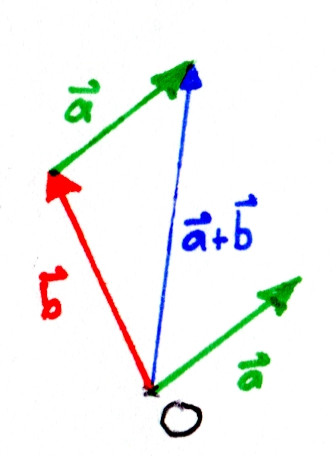
\includegraphics[scale=0.8]{LAGrundlagen1Rechengesetze}
    \caption{Summe zweier Vektoren}
  \end{marginfigure}
  %
  Bei Multiplikation mit dem Faktor $r$ wird der Pfeil einfach länger oder kürzer.
  Bei Addition von zwei Vektoren ergibt sich der Pfeil durchs Hintereinanderzeichnen der zwei Anfangspfeile.
  \begin{enumerate}
    \item $\vec{a} + \vec{b} = \vec{b} + \vec{a} = \begin{pmatrix}
      a_1 + b_1 \\ a_2 + b_2 \\ a_3 + b_3
    \end{pmatrix}$
    \item $r * \vec{a} =
    \begin{pmatrix}
      r * a_1 \\ r* a_2 \\ r * a_3
    \end{pmatrix}$
    \item $r * (\vec{a} + \vec{b}) = r*\vec{a} + r*\vec{b}$
  \end{enumerate}
\end{bla}

\begin{bla}{Strecken und Längen}
  %
  \begin{marginfigure}[10em]
    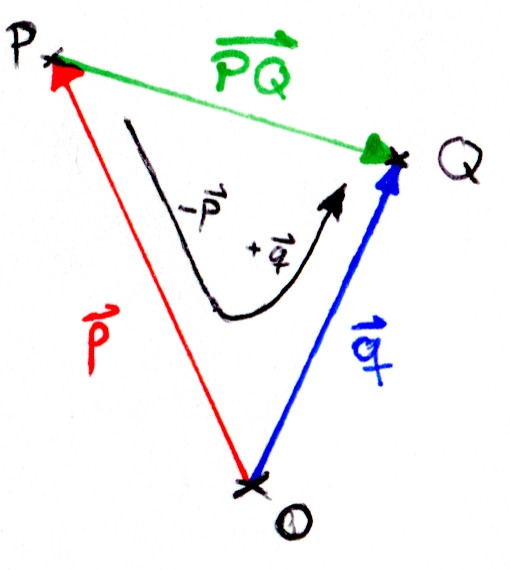
\includegraphics[scale=0.6]{LAGrundlagen2Strecken}
    \caption{Strecke von $P$ nach $Q$}
  \end{marginfigure}
  %
  Die Strecke zwischen zwei Punkten $\overrightarrow{PQ}$ bekommt man, indem man erst von $P$ rückwärts zum Ursprung geht ($-\vec{p}$) und dann (mit $\vec{q}$) vom Ursprung zu $Q$:
  \begin{equation*}
    \overrightarrow{PQ} = - \vec{p} + \vec{q} = \begin{pmatrix}
      q_1\\q_2\\q_3
    \end{pmatrix}
    -
    \begin{pmatrix}
      p_1\\p_2\\p_3
    \end{pmatrix}
    =
    \begin{pmatrix}
      q_1 - p_1 \\ q_2 - p_2 \\ q_3 - p_3
    \end{pmatrix}
  \end{equation*}

  Der Betrag einer Stecke oder die Länge eines Vektors ergeben sich ähnlich zum Satz des Pythagoras:
  \begin{equation*}
    |\overrightarrow{PQ}| = \sqrt{(q_1 - p_1)^2 + (q_2 - p_2)^2 + (q_3 - p_3)^2}
  \end{equation*}
   \begin{marginfigure}
    \begin{tcolorbox}[colback=white!95!black,colframe=white!75!black,title=CAS:,arc=0mm]
      \begin{scriptsize}
        \textbf{Calculator}: \\*
        \menu{Menü > Mat. und Vek > Normen > Norm}
        \( \leadsto \) \textsc{norm}\( \left( \left[ \begin{smallmatrix}
          0 \\ 0 \\ 1
        \end{smallmatrix} \right] \right) \leadsto 1 \)
      \end{scriptsize}
    \end{tcolorbox}
  \end{marginfigure}
\end{bla}

\section{Produkte}
Das Multiplizieren von Vektoren ist ein bisschen komplizierter als bei normalen Zahlen, durch Vektoren zu Teilen ist sogar gar nicht möglich.

\begin{bla}{Skalarprodukt}
   \begin{marginfigure}[5em]
    \begin{tcolorbox}[colback=white!95!black,colframe=white!75!black,title=CAS:,arc=0mm]
      \begin{scriptsize}
        \textbf{Calculator}: \\*
        \menu{Menü > Mat. und Vek > Vek. > SKP} \\*
        \( \leadsto \) \textsc{dotP}\( \left( \left[ \begin{smallmatrix}
          1 \\ 1 \\ 1
        \end{smallmatrix} \right], \left[ \begin{smallmatrix}
          1 \\ 1 \\ 1
        \end{smallmatrix} \right] \right) \leadsto 3 \)
      \end{scriptsize}
    \end{tcolorbox}
  \end{marginfigure}
  Eine hilfreiche Methode um Winkel zu bestimmen ist das sogenannte \emph{Skalarprodukt}:
  \begin{equation*}
    \vec{a} * \vec{b} = (a_1*b_1) + (a_2*b_2) + (a_3*b_3) = |\vec{a}|*|\vec{b}|*\cos(\varphi)
  \end{equation*}
  Hier ist $\varphi$ der Winkel zwischen den beiden Vektoren.
  Das Ergebnis des Skalarproduktes ist ein Skalar, also eine Zahl.
  \\
  Eine sinnvolle Anwendung ist die Suche nach rechten Winkeln:\\
  Wegen des Cosinus ist:
  \begin{equation*}
    \vec{a} * \vec{b} = 0
    \Leftrightarrow
    \varphi = 90\degree
  \end{equation*}
\end{bla}

\begin{bla}{Kreuzprodukt}
   \begin{marginfigure}[5em]
    \begin{tcolorbox}[colback=white!95!black,colframe=white!75!black,title=CAS:,arc=0mm]
      \begin{scriptsize}
        \textbf{Calculator}: \\*
        \menu{Menü > Mat. und Vek > Vek. > Kreuzprod} \\*
        \( \leadsto \) \textsc{crossP}\( \left( \left[ \begin{smallmatrix}
          1 \\ 1 \\ 1
        \end{smallmatrix} \right], \left[ \begin{smallmatrix}
          1 \\ 1 \\ 1
        \end{smallmatrix} \right] \right) \leadsto \left[ \begin{smallmatrix}
          0 \\ 0 \\ 0
        \end{smallmatrix} \right] \)
      \end{scriptsize}
    \end{tcolorbox}
  \end{marginfigure}
  \begin{marginfigure}[0em]
    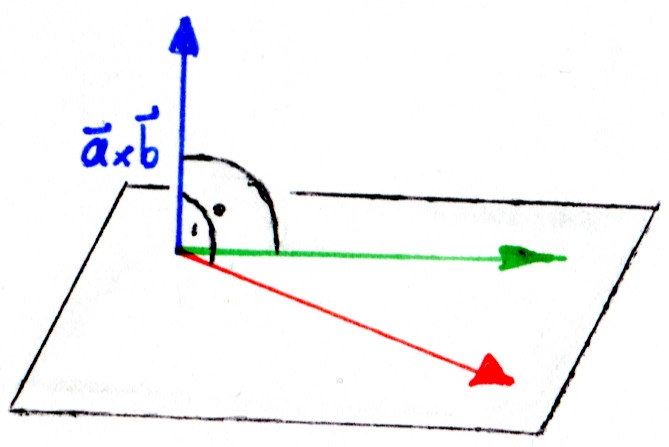
\includegraphics[scale=0.6]{LAGrundlagen3Kreuzprodukt}
    \caption{Kreuzprodukt}
  \end{marginfigure}
Beim \emph{Kreuzprodukt} aus zwei Vektoren ergibt sich ein neuer Vektor:
  \begin{equation*}
      \vec{a} \times \vec{b} =
      \begin{pmatrix}
      a_2 * b_3 - a_3 * b_2 \\
      a_3 * b_1 - a_1 * b_3 \\
      a_1 * b_2 - a_2 * b_1 \\
    \end{pmatrix}
    = - \vec{b} \times \vec{a}
  \end{equation*}
  Dieser neue Vektor steht senkrecht auf den anderen beiden und hat die Länge:
  \begin{equation*}
    |\vec{a} \times \vec{b}| = |\vec{a}| * |\vec{b}| * \sin(\varphi)
  \end{equation*}
\end{bla}

\clearpage

\begin{bla}{Lineare Abhängigkeit}
  Durch Verlängern und Verkürzen eines Vektors $\vec{a}$ kann man eine ganze Gerade erreichen:
  \[
  \text{g: }\ \vec{x} = k * \vec{a}
  \]
  Nimmt man einen zweiten Vektor $\vec{b}$ dazu, gibt es zwei Möglichkeiten:
  %
  \begin{marginfigure}[0em]
    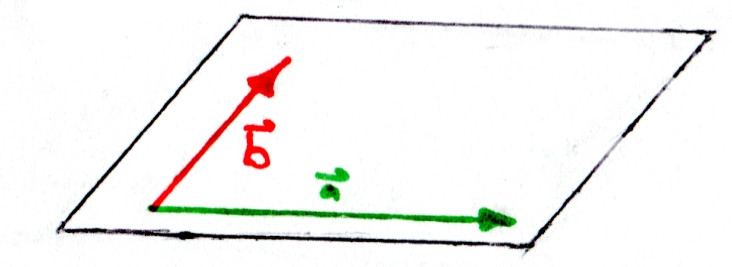
\includegraphics[scale=0.6]{LAGrundlagen4LinAbh1}
    \caption{Zwei linear unabhängige Vektoren spannen eine Ebene auf}
  \end{marginfigure}
  %
  \begin{itemize}
    \item \textbf{$\vec{a}$ und $\vec{b}$ sind parallel:} \\
    Man nennt die beiden \emph{linear abhängig}, weil man immer noch nur die Gerade erreichen kann:
    \[
    \text{g: }\ \vec{x} = k * \vec{a} +  l * \vec{b} =  k * \vec{a}
    \]
    \item \textbf{$\vec{a}$ und $\vec{b}$ laufen in verschiedene Richtungen:} \\
    Man nennt die beiden jetzt \emph{linear unabhängig}, weil man plötzlich eine ganze Ebene erreichen kann:
    \[
    \text{E: }\ \vec{x} = k * \vec{a} +  l * \vec{b}
    \]
  \end{itemize}

  %
  \begin{marginfigure}[-17em]
    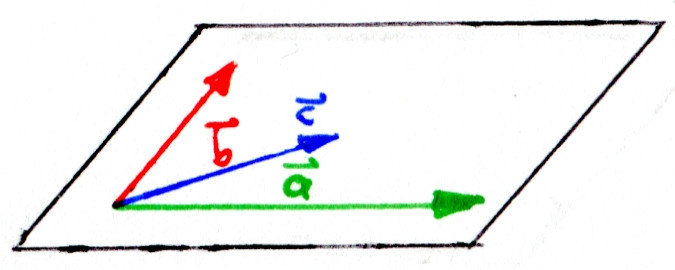
\includegraphics[scale=0.6]{LAGrundlagen4LinAbh2}
    \caption{Drei linear abhängige Vektoren spannen keinen Raum, sondern nur eine Ebene oder Gerade auf}
  \end{marginfigure}
  %
  %
  \begin{marginfigure}
    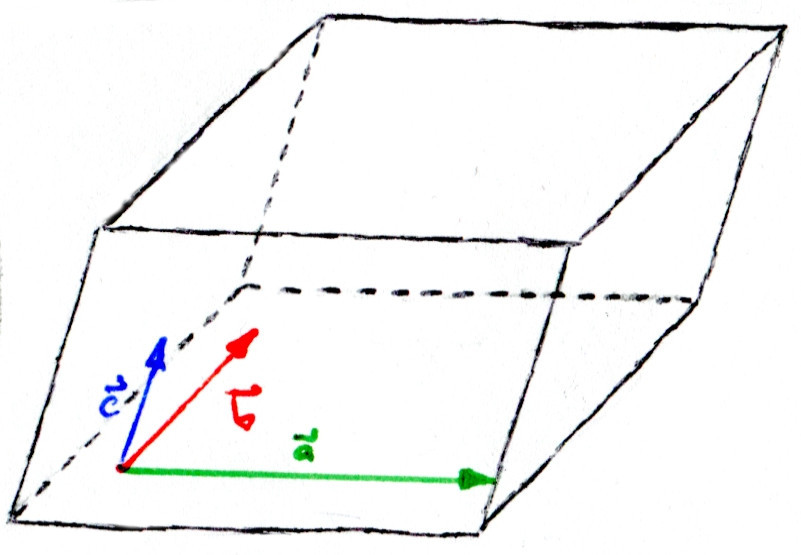
\includegraphics[scale=0.6]{LAGrundlagen4LinAbh3}
    \caption{Drei linear unabhängige Vektoren spannen den gesamten Raum auf}
  \end{marginfigure}
  %
  Als nächstes kann man noch einen dritten Vektor dazunehmen.
  Man nennt die drei dann \emph{linear unabhängig}, wenn man alle Punkte im ganzen Raum erreichen kann und \emph{linear abhängig}, falls man nur eine Ebene oder Gerade erreicht.
\end{bla}

\chapter{Objekte im Raum}
\begin{inhalt}
  \begin{itemize}
    \item Geraden
    \item Ebenen: Parameter-, Normalen-, Koordinatendarstellung
    \item Darstellungsformen untereinander umformen
  \end{itemize}
\end{inhalt}

\begin{bla}{Geraden}
  %
  \begin{marginfigure}[0em]
    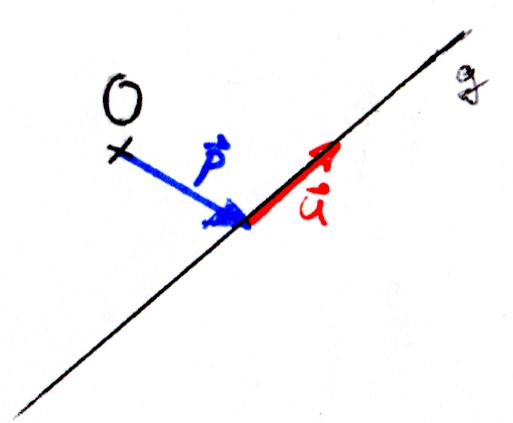
\includegraphics[scale=0.8]{AGLage_Gerade}
    \caption{Gerade, Richtung $\vec{u}$, stützt sich auf $\vec{p}$}
  \end{marginfigure}
  %
  Eine Gerade g die durch den Punkt $P$ in Richtung $\vec{u}$ läuft kann geschrieben werden als:
  \begin{equation*}
    \text{g: }\ \vec{x} = \vec{p} + \text{r} * \vec{u}\text{, mit r}\in\R
  \end{equation*}
  Die Vorstellung dazu ist, dass man alle Punkte $\vec{x}$ auf der Geraden trifft, indem man von $P$ aus den Vektor $\vec{u}$ verlängert oder verkürzt.
\end{bla}

\begin{bla}{Ebenen - Parameterdarstellung}
  %
  \begin{marginfigure}[0em]
    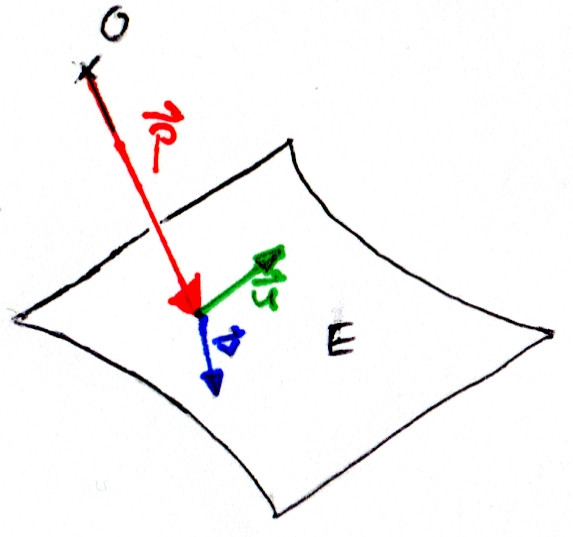
\includegraphics[scale=0.8]{AGLage_EbeneParam}
    \caption{Ebene, aufgespannt durch $\vec{u}$ und $\vec{v}$, stützt sich auf $\vec{p}$}
  \end{marginfigure}
  %
  Genauso kann man auch Ebenen darstellen, nur dass man von $P$ aus in zwei Richtungen gehen kann:
  \begin{equation*}
    \text{E: }\ \vec{x} = \vec{p} + \text{r} * \vec{u} + \text{s} * \vec{v} \text{, mit r, s} \in \R
  \end{equation*}
  $\vec{u}$ und $\vec{v}$ nennt man \emph{Spannvektoren} der Ebene E.
\end{bla}

\begin{bla}{Ebenen - Normalendarstellung}
  %
  \begin{marginfigure}[0em]
    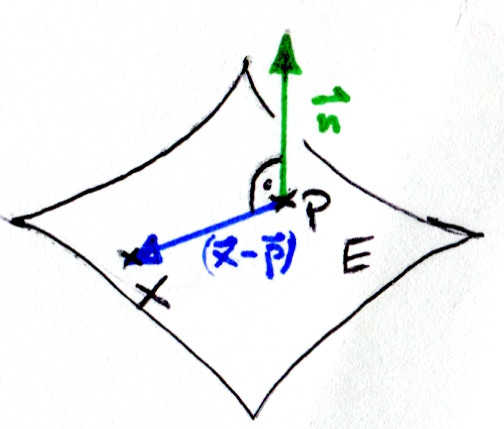
\includegraphics[scale=0.8]{AGLage_EbeneNormal}
    \caption{Ebene senkrecht zu $\vec{n}$, ausgehend von Stützpunkt $P$}
  \end{marginfigure}
  %
  Zu jeder Ebene gehört ein Vektor, der senkrecht darauf steht.

  Der sogenannte \emph{Normalenvektor} steht dann auch senkrecht auf allen Linien, die in der Ebene liegen.

  Eine Ebene E beschreibt man damit wie folgt:
  \begin{equation*}
    \text{E: }\ \left( \vec{x} - \vec{p} \right) * \vec{n} = 0
  \end{equation*}
  $\vec{x} - \vec{p}$ ist die Verbindung $\overrightarrow{PX}$ zwischen X und der Stützstelle P.
  Diese Verbindung liegt in der Ebene, und steht damit senkrecht auf $\vec{n}$. Das Skalarprodukt ist Null.
\end{bla}



\begin{bla}{Ebenen - Koordinatendarstellung}
  \label{AG:E-Koordinatendarst}
  Wenn man die Normalendarstellung ausmultipliziert, ergibt sich folgende Gleichung für E:
  \begin{align*}
    \vec{x} * \vec{n} &= \vec{p} * \vec{n}\\
    n_1*x_1 + n_2*x_2 + n_3*x_3 &= c
  \end{align*}
  $\vec{p} * \vec{n}$ lässt sich ausrechnen und ergibt die Zahl $c$.

  Diese Darstellung ist nicht so offensichtlich aus Vektoren aufgebaut, aber sehr hilfreich um einige Aufgaben auszurechnen.
\end{bla}

\begin{bla}{Ebenen - \textsc{Hesse}'sche Normalenform}
  Die Gleichungen der Normalen- und Koordinatendarstellung können durch den Betrag des Normalenvektors geteilt werden:
  \begin{align*}
    \text{E: }\ \frac{ \left(n_1*x_1 + n_2*x_2 + n_3*x_3\right)}{|\vec{n}|} - \frac{c}{|\vec{n}|}
    &=
    0
    \\
    \text{E: }\ \frac{\left( \vec{x} - \vec{p} \right) * \vec{n}}{|\vec{n}|}
    &=
    0
  \end{align*}

  Die Darstellung wird im nächsten Kapitel sehr praktisch zur Abstandsbestimmung sein.
\end{bla}

\section{Ebenengleichungen aus Punkten}
Gesucht werden im Folgenden die Ebenengleichungen wenn drei Punkte $A,B,C$ beziehungsweise $\vec{a}, \vec{b}, \vec{c}$ im Raum gegeben sind.

\begin{bla}{Stützvektor}
  Der Stützvektor muss einfach irgendeinen Punkt auf der Ebene treffen, also kann man zum Beispiel $\vec{a}$ aussuchen.
\end{bla}

\begin{bla}{Spannvektoren}
  Die Spannvektoren sind irgendwelche zwei Vektoren, die in der Ebene oder parallel dazu laufen. Wir haben zur Auswahl: $\overrightarrow{AB}$, $\overrightarrow{BC}$ und $\overrightarrow{AC}$.

  \textbf{Wichtig: Lineare Unabhängigkeit:} Wenn nur zwei Punkte gegeben sind, oder die drei Punkte auf einer Geraden liegen haben wir nicht genügend verschiedene Vektoren um eine Ebene zu basteln.
  Man erkennt das daran, dass die Vektoren in die gleiche Richtung zeigen, nur verschieden lang sind
  (Das Kreuzprodukt ist dann Null).
\end{bla}

\begin{bla}{Normalenvektor}
  Kennt man schon zwei verschiedene Spannvektoren, bekommt man den Normalenvektor über deren Kreuzprodukt.

  Man kann stattdessen aber auch die Koordinatengleichung für Ebenen benutzen:
  \begin{equation*}
    n_1x_1 + n_2x_2 + n_3x_3 = b
  \end{equation*}



  Setzt man jetzt zum Beispiel die Punkte $A=(1|1|0), B=(1|0|1), C=(0|0|1)$ für $\vec{x}$ ein, ergeben sich die Gleichungen:
  \begin{align*}
    n_1 + n_2 &= b \\
    n_1 + n_3 &= b \\
    n_2 + n_3 &= b \\
    \text{Es folgt: } n_1 = n_2 = n_3 &= \frac{1}{2} * b
  \end{align*}
  Man wählt dann $b$ irgendwie und hat nicht nur den Normalenvektor, sondern gleich die dazu passende Koordinatengleichung.
\end{bla}

So konstruiert man die Koordinatengleichung, für die beiden anderen Gleichungen muss man nur die entsprechenden Vektoren an der richtigen Stelle einsetzen.

\section{Ebenengleichungen aus Ebenengleichungen}
\begin{bla}{Parameter- zu Normalenform}
  Eine Parameterform ist gegeben:
  \[
  \text{E: }\ \vec{p} + r * \vec{u} + s * \vec{v} \text{, mit }r,s \in \R
  \]
  Für die Normalenform brauchen wir einen Normalenvektor $\vec{n}$, der senkrecht auf den beiden Spannvektoren steht: $\vec{n} * \vec{u} = 0$ und $\vec{n}*\vec{v} = 0$

  Die Spannvektoren sind bekannt, also kann man die Gleichungen ausmultiplizieren und bekommt ein LGS für $n_1, n_2$ und $ n_3$.
  Zwei Gleichungen für drei Variablen liefern kein eindeutiges Ergebnis, also muss man am Schluss eine der drei Variablen selbst festlegen.

  Stattdessen kann man auch einfach $\vec{u} \times \vec{v} = \vec{n}$ ausrechnen.

  Der Stützvektor kann gleich bleiben.
\end{bla}

\begin{bla}{Koordinaten- zu Normalenform}
  \label{5_UmformungKN}
  Die Vorfaktoren vor den $x$-Werten sind die Komponenten des Normalenvektors.

  Um einen Stützvektor zu finden setzt man in der Koordinatenform ein paar $x$-Werte zu irgendeiner festen Zahl, so dass man einen Punkt ablesen kann.
  \begin{align*}
    x_1 + 2*x_2 -2 * x_3 &= 5\\
    \text{Setze $x_2 = 2$ und $x_3 = 0$: }\ x_1 + 4 &= 5\\
    \text{Es ergibt sich: } \vec{p} =
    \begin{pmatrix}
      x_1\\x_2\\x_3
    \end{pmatrix}
    &=
    \begin{pmatrix}
      1 \\ 2 \\ 0
    \end{pmatrix}
  \end{align*}
\end{bla}

\begin{bla}{Normalen- zu Koordinatenform}
  Das Skalarprodukt wird ausmultipliziert (siehe \ref{AG:E-Koordinatendarst}).
\end{bla}



\begin{bla}{Koordinaten- zu Parameterdarstellung}
  Einen Stützvektor findet man wie in \ref{5_UmformungKN} durch Einsetzen.

  Um Spannvektoren zu bekommen, suchen wir alle Vektoren $\vec{v}$, die auf $\vec{n}$ senkrecht stehen:
  \begin{align*}
    \vec{v} * \vec{n} &= 0\\
    n_1v_1 + n_2v_2 + n_3v_3 &= 0
  \end{align*}
  Um nicht parallele Spannvektoren zu bekommen setzen wir oben zum Beispiel einmal $v_2 = 0, v_3 = 1$ und einmal $v_2 = 1, v_3 = 0$, lösen damit die Gleichung und erhalten zwei Spannvektoren.
\end{bla}

\chapter{Lagebeziehungen}
\begin{inhalt}
  Wie liegen zueinander:
  \begin{itemize}
    \item Punkt-Gerade, Punkt-Ebene
    \item Gerade-Gerade, Gerade-Ebene
    \item Ebene-Ebene
  \end{itemize}
\end{inhalt}

\begin{bla}{Punktproben}
  Um zu sehen ob ein Punkt auf einer Geraden oder Ebene liegt, setzt man seine Koordinaten in deren Gleichungen ein.
  Es ergibt sich entweder eine wahre Aussage ($0=0$ - Punkt liegt auf der Geraden) oder eine falsche ($10 = 10.5$ - Punkt liegt nicht auf der Geraden)
\end{bla}

\begin{bla}{Gerade - Gerade}
  \begin{align*}
    \text{g: }\ \vec{x} &= \vec{p} + r * \vec{u} \\
    \text{h: }\ \vec{x} &= \vec{q} + s * \vec{v}
  \intertext{Man sucht Punkte, die auf beiden Geraden liegen.
  Dazu setzt man das $\vec{x}$ der beiden gleich.
  Man erhält ein LGS für die beiden Parameter:}
    \vec{p} + r * \vec{u} &= \vec{q} + s * \vec{v}
\end{align*}
  Sucht man jetzt Lösungen für $r$ und $s$, kann man folgende Ergebnisse bekommen:
  %
  \begin{marginfigure}[-10em]
    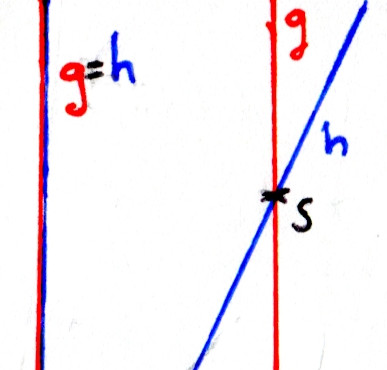
\includegraphics[scale=0.8]{AGLage_GerGerKontakt}
    \caption{Sich berührende Geraden}
  \end{marginfigure}
  %
  %
  \begin{marginfigure}[0em]
    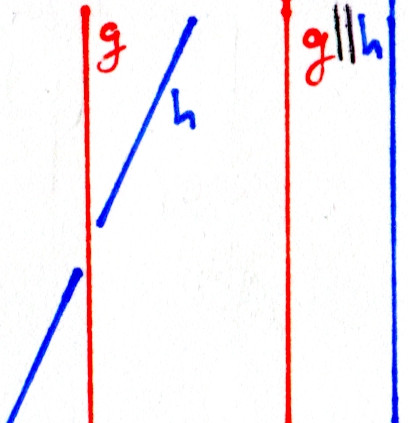
\includegraphics[scale=0.8]{AGLage_GerGerVorbei}
    \caption{Sich nicht berührende Geraden}
  \end{marginfigure}
  %
  \begin{itemize}
    \item $\infty$ \textbf{Lösungen}: Die Geraden sind \emph{identisch}.
    \item \textbf{Eine Lösung}: Es gibt einen \emph{Schnittpunkt} S.
    Er wird berechnet, indem man die Lösung für $k$ oder $l$ in die jeweilige Geradengleichung einsetzt.
    \item \textbf{Keine Lösung}: Die Geraden sind \emph{parallel} wenn die Richtungsvektoren linear abhängig sind.
    Wenn nicht, nennt man sie \emph{windschief}.
  \end{itemize}
\end{bla}

\begin{bla}{Gerade - Ebene}
  \label{AG_LageGE}
  Man setzt die Geradengleichung in die Ebenengleichung ein:
  \begin{align*}
    \text{g: }\ &\vec{x} = \vec{p} + \text{k} * \vec{u}
    \\
    \text{E: }\ &n_1x_1 + n_2x_2 + n_3x_3 = b
    \intertext{Das $\vec{x}$ aus g wird in E eingesetzt:}
    n_1(p_1 + k * u_1) + &n_2(p_2 + k * u_2) + n_3(p_3 + k * u_3) = b
  \end{align*}
  Alles bis auf k ist bekannt.
  Wie oben gibt es wieder verschiedene Lösungen für k:
  %
  \begin{marginfigure}[-30em]
    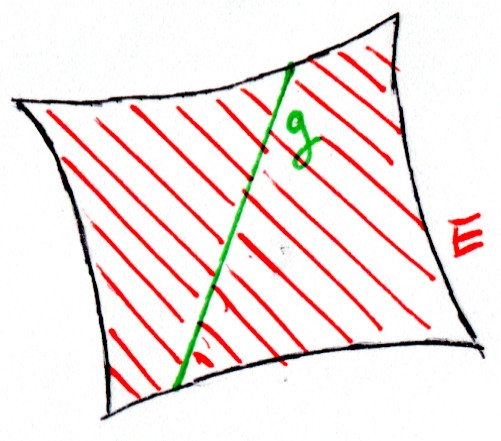
\includegraphics[scale=0.8]{AGAbstand_EbGerIdentisch}
    \caption{Gerade die in einer Ebene verläuft}
  \end{marginfigure}
  %
  %
  \begin{marginfigure}[-7.3em]
    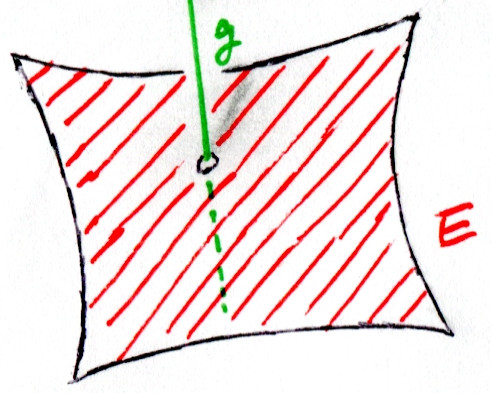
\includegraphics[scale=0.8]{AGAbstand_EbGerSchnitt}
    \caption{Gerade schneidet Ebene}
  \end{marginfigure}
  %
  %
  \begin{marginfigure}[0em]
    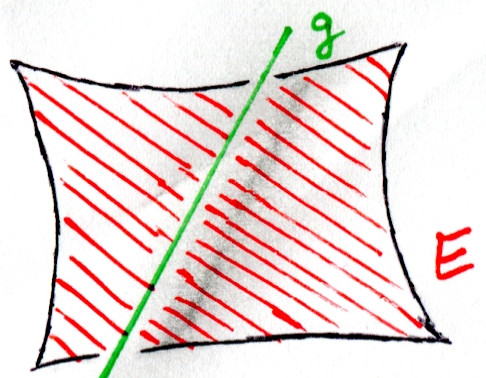
\includegraphics[scale=0.8]{AGAbstand_EbGerParallel}
    \caption{Gerade parallel zu Ebene}
  \end{marginfigure}
  %
  \begin{itemize}
    \item \textbf{Eine Lösung} ($k=2$): Es gibt einen \emph{Schnittpunkt} S.
    Er wird berechnet, indem man die Lösung für $k$ in die Geradengleichung einsetzt.
    \item \textbf{Wahre Aussage} ($1=1$): Die Gerade \emph{liegt in} der Ebene.
    \item \textbf{Widerspruch} ($1=27$): Gerade und Ebene sind \emph{parallel}.
  \end{itemize}
\end{bla}

\begin{bla}{Ebene - Ebene}
  Man setzt die $\vec{x}$ aus den Ebenengleichungen gleich und erhält ein LGS.
  %
  \begin{marginfigure}[0em]
    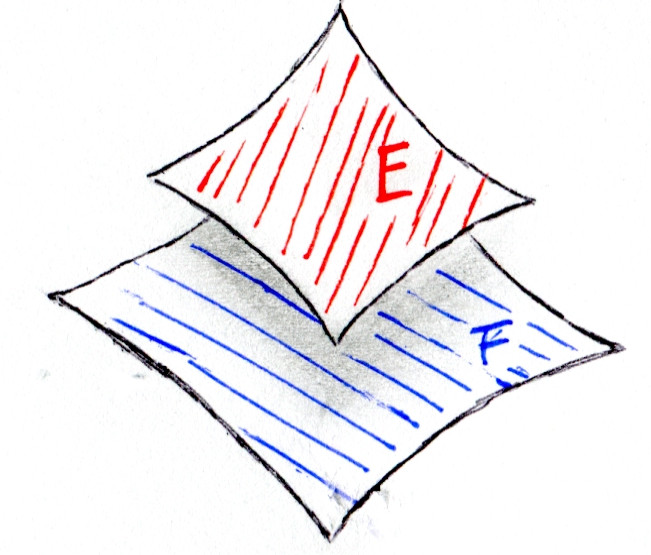
\includegraphics[scale=0.8]{AGLage_EbEbParallel}
    \caption{Parallele Ebenen}
  \end{marginfigure}
  %
  %
  \begin{marginfigure}[0em]
    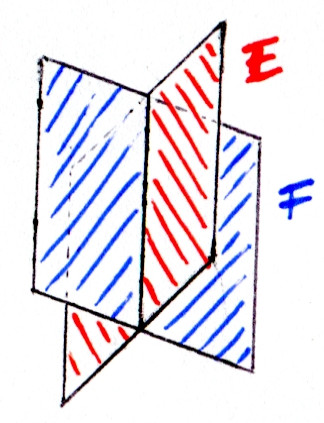
\includegraphics[scale=1.2]{AGLage_EbEbSchnitt}
    \caption{Ebenen mit Schnittgerade}
  \end{marginfigure}
  %
  \begin{itemize}
    \item Ergibt sich ein \textbf{Widerspruch}, so sind die Ebenen parallel.
    \item Ergibt sich eine \textbf{unendliche Lösung}, so liefert die Lösung die Schnittgerade der beiden Ebenen.
  \end{itemize}

  Hat man die Ebenen in Koordinaten- oder Normalenform vorliegen, so kann man auch die beiden Normalenvektoren in ein Kreuzprodukt schreiben.
  Das Ergebnis ist der Richtungsvektor der Schnittgeraden oder Null, falls die Ebenen parallel sind.
  Dann braucht man noch einen einzigen Stützpunkt, der in beiden Ebenen liegt und hat die Schnittgerade bestimmt.
\end{bla}

%adpitub
\chapter{Abstände}
\begin{inhalt}
  Abstände zwischen
  \begin{itemize}
    \item Punkt-Punkt, Punkt-Gerade, Punkt-Ebene
    \item Gerade-Gerade, Gerade-Ebene
    \item Ebene-Ebene
  \end{itemize}
\end{inhalt}

Abstände zwischen Objekten im Raum schreibt man $d(\text{Ding}_1, \text{Ding}_2)$

\begin{bla}{Punkt - Punkt}
  Der Abstand zweier Punkte $P,Q$ ist die Länge des Vektors $\overrightarrow{PQ}$:
  \[
  d(P,Q)
  =
  \left| \overrightarrow{PQ} \right|
  =
  \left|\begin{pmatrix}
    q_1 - p_1 \\ q_2 - p_2 \\ q_3 - p_3
  \end{pmatrix}\right|
  =
  \sqrt{(q_1 - p_1)^2 + (q_2 - p_2)^2 + (q_3 - p_3)^2}
  \]
\end{bla}

\begin{bla}{Punkt - Gerade: Laufender Punkt}
  \[
  \text{g: }\ \vec{x} = \vec{p} + r * \vec{u}
  \]
  Der Abstand zwischen Punkt $P$ und der Geraden $g$ ergibt sich, indem man den Abstand zwischen $P$ und einem beliebigen Punkt $Q$ auf der Gerade ausrechnet.
  Setzt man also für $Q$ die Geradengleichung ein, hängt $\overrightarrow{PQ}$ noch von dem Parameter r ab.
  Jetzt sucht man den Vektor, der senkrecht auf dem Richtungsvektor $\vec{u}$ der Geraden steht, also
  \[
  \overrightarrow{PQ} * \vec{u} = 0
  \]
  Man findet ein $r$ als Lösung der Gleichung.
  Damit hat man den Punkt $Q$ mit dem kürzesten Abstand und errechnet dann $d(P,Q)$.
\end{bla}



\begin{bla}{Punkt - Gerade: Hilfsebene}
  %
  \begin{marginfigure}[0em]
    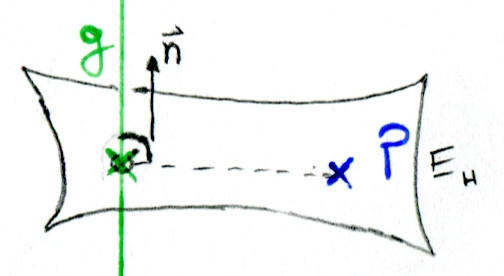
\includegraphics[scale=0.8]{AGAbstand_PktGerHilfsebene}
    \caption{Hilfsebene durch $P$, senkrecht zu Gerade g}
  \end{marginfigure}
  %
  Man baut sich eine Ebene E$_\text{H}$ senkrecht zu g, die durch $P$ geht:

  Damit die Gerade senkrecht auf der Ebene steht wählt man als Normalenvektor $\vec{n}$ der Ebene den Richtungsvektor der Geraden, $\vec{u}$.

  Damit die Ebene durch $P$ geht, wählt man $\vec{p}$ einfach als Stützvektor.

  Der Schnittpunkt zwischen Gerade und der neuen Ebene wird jetzt S genannt und kann einfach berechnet werden (siehe \ref{AG_LageGE}).

  Der Abstand vereinfacht sich zu:
  $d(P,g) = d(P,S)$
\end{bla}

\begin{bla}{Punkt - Ebene: Lotgerade}
  %
  \begin{marginfigure}[5em]
    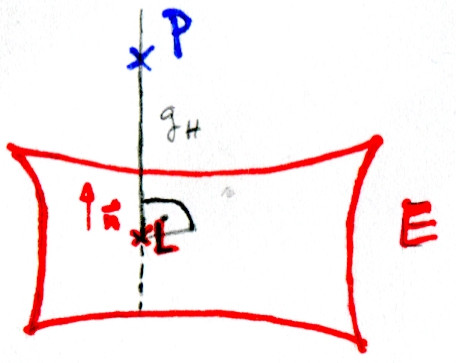
\includegraphics[scale=0.8]{AGAbstand_PktEbLotgerade}
    \caption{Lotgerade, senkrecht zur Ebene E, durch Punkt $P$}
  \end{marginfigure}
  %
  Man baut sich eine Gerade g$_\text{H}$, die durch P geht und senkrecht auf E steht:

  Als Stützvektor wählen wir $\vec{p}$, dann geht die Gerade durch P.

  Als Richtungsvektor wählen wir den Normalenvektor der Ebene: $\vec{n}$.

  Gesucht ist dann zuletzt der sogenannte \emph{Lotfußpunkt}: Der Schnittpunkt der Geraden mit der Ebene.
  Wir nennen ihn $L$ und finden ihn mit \ref{AG_LageGE}.

  Der Abstand vereinfacht sich dann auf zwei Punkte:
  $d(P,E) = d(P,L)$
\end{bla}

\begin{bla}{Punkt - Ebene: \textsc{Hesse}sche Normalenform}
  In der \textsc{Hesse}schen Normalenform kann der Punkt $P$ einfach auf der linken Seite der Gleichung eingesetzt werden, dann ergibt sich rechts der Abstand zur Ebene:
  \[
  \frac{ \left(n_1*x_1 + n_2*x_2 + n_3*x_3\right) - c}{|\vec{n}|}
  = d(P,E)
  \]
\end{bla}

\begin{bla}{Windschiefe Geraden: Laufende Punkte}
  Die beiden Geraden g und h sind windschief und wir suchen den Abstand:
  \begin{align*}
    \text{g: }\ \vec{x} = \vec{p} + r * \vec{u} \\
    \text{h: }\ \vec{x} = \vec{q} + s * \vec{v}
  \end{align*}
  Man nimmt zwei beliebige Punkte aus den Geradengleichungen und nennt sie zum Beispiel $G$ aus g und $H$ aus h.

  Deren Abstandsvektor $\overrightarrow{GH}$ hängt noch von $r$ und $s$ ab.
  Der kleinste Abstand ist der, bei dem $\overrightarrow{GH}$ auf beiden Richtungsvektoren $\vec{u}$ und $\vec{v}$ senkrecht steht:
  \begin{align*}
    \overrightarrow{GH} * \vec{u} = 0 \\
    \overrightarrow{GH} * \vec{v} = 0
  \end{align*}
  Dieses LGS hat zwei Gleichungen und liefert uns damit $r$ und $s$.

  Diese beiden setzen wir einfach in $\overrightarrow{GH}$ ein und haben den Abstandsvektor.
\end{bla}



\begin{bla}{Windschiefe Geraden: Hilfsebene}
  %
  \begin{marginfigure}[0em]
    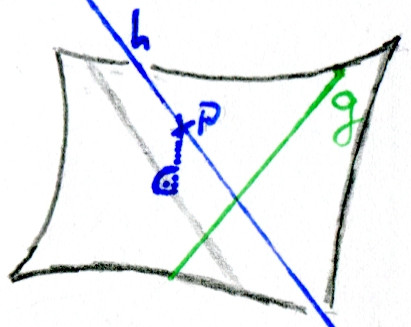
\includegraphics[scale=0.8]{AGAbstand_GerGerWindschief}
    \caption{Hilfsebene E, parallel zu beiden Geraden, g liegt in E}
  \end{marginfigure}
  %
  Die beiden Geraden g und h sind windschief und wir suchen den Abstand:
  \begin{align*}
    \text{g: }\ \vec{x} &= \vec{p} + r * \vec{u} \\
    \text{h: }\ \vec{x} &= \vec{q} + s * \vec{v}
    \intertext{Man konstruiert eine Ebene die parallel zu beiden Geraden liegt und die Gerade g sogar enthält:}
    \text{E}_\text{H} \text{: }\ \vec{x} &= \vec{p} + k * \vec{u} + l * \vec{v}
\end{align*}
  Die Gerade h hat zur ganzen Ebene den gleichen Abstand, also nimmt man einfach einen Punkt $P$ aus h und sucht den Abstand zur Ebene:
  \[
  d(\text{g},\text{h}) = d(P,\text{E})
  \]
\end{bla}

\begin{bla}{Parallele Geraden}
  Der Abstand ist entlang der gesamten Geraden gleich.
  Man nimmt aus einer Geraden einen beliebigen Punkt und berechnet den Abstand des Punktes zu der anderen Geraden.
\end{bla}

\begin{bla}{Gerade - Ebene}
  Abstände ergeben hier nur Sinn, wenn Gerade und Ebene parallel sind, weil sie sich sonst schneiden.

  Man sucht aus der Geraden einfach irgendeinen Punkt raus und rechnet dann den Abstand Punkt - Ebene.
\end{bla}

\begin{bla}{Ebene - Ebene}
  Abstände ergeben hier nur Sinn, wenn die Ebenen parallel sind, weil sie sich sonst schneiden.

  Man sucht aus einer der Ebenen einfach irgendeinen Punkt raus und rechnet dann den Abstand Punkt - Ebene.
\end{bla}

\chapter{Winkel und Spiegelungen}
\begin{inhalt}
  Winkel zwischen
  \begin{itemize}
  	\item Vektoren,
    \item Geraden,
    \item Ebenen,
    \item Gerade und Ebene
  \end{itemize}
%  Spiegelung von
%  \begin{itemize}
%  	\item Punkt, Gerade und Ebene an Gerade,
%  	\item Punkt, Gerade und Ebene an Ebene.
%  \end{itemize}
\end{inhalt}

Für die Winkel zwischen Objekten schreiben wir $\angle(\text{Ding}_1,\text{Ding}_2)$.

\begin{bla}{Skalarprodukt}
	Aus dem Skalarprodukt zwischen zwei Vektoren ergibt sich eine Winkelbeziehung:
	\[
	\vec p * \vec q = |\vec p| * |\vec q| * \cos\left(\angle\left(\vec p, \vec q\right)\right)
	\]

	Einfacher schreibt man oft:
	\[
	\frac{\vec p * \vec q }{ |\vec p| * |\vec q| } = \cos\left(\angle\left(\vec p, \vec q\right)\right)
	\]
\end{bla}

\begin{bla}{Kreuzprodukt}
	Das Kreuzprodukt funktioniert ähnlich:
	\[
	| \vec p \times \vec q | = |\vec p| * |\vec q| * \sin\left(\angle\left(\vec p, \vec q\right)\right)
	\]
	Da das Kreuzprodukt einen Vektor liefert, muss man hier noch den Betrag ausrechnen.
\end{bla}

\clearpage

\begin{bla}{Geraden}
	Der Winkel zwischen zwei Geraden ist der Winkel zwischen ihren Richtungsvektoren.

	Wenn sich dabei ein Winkel größer als \SI{90}{\degree} ergibt, muss man für ein sinnvolles Ergebnis diese \SI{90}{\degree} wieder abziehen.
	Alternativ kann man auch $$| \vec p * \vec q |$$ \emph{mit Betragsstrichen} bei der Rechnung verwenden, dann ergibt sich automatisch der kleinere Winkel.
\end{bla}

\begin{bla}{Ebenen}
	Der Winkel zwischen zwei Ebenen ist genau der Winkel zwischen ihren Normalenvektoren:
	\[
	\angle(E_1,E_2) = \angle(n_1,n_2)
	\]
\end{bla}

\begin{bla}{Gerade-Ebene}
	Man bekommt den Winkel zwischen einer Geraden und einer Ebenen, indem man den zwischen dem Richtungsvektor der Geraden und dem Normalenvektor der Ebenen berechnet.
	Diesen Winkel muss man noch von \SI{90}{\degree} abziehen.

	Man kann sich den zweiten Rechenschritt sparen, indem man statt eines Cosinus einen Sinus verwendet:
	\begin{align*}
	\angle(g,E) = \SI{90}{\degree} - \angle(\vec u_g, \vec n_E)
	&= \SI{90}{\degree} - \cos^{-1} \left( \frac {\vec u_g * \vec n_E }{ |\vec u_g| * |\vec n_E| } \right)
	\\
	&= \sin^{-1} \left( \frac {\vec u_g * \vec n_E }{ |\vec u_g| * |\vec n_E| } \right)
	\end{align*}
\end{bla}

\begin{bla}
	{Spiegelungen}
	Für eine Spiegelung eines Punktes an etwas anderem muss zuerst der Spiegelpunkt gefunden werden.
	\\
	Spiegelt man also einen Punkt $P$ an einer Geraden oder Ebene, möchte man darauf einen Punkt $F$ finden, so dass $\overrightarrow{PF}$ senkrecht auf der Ebene oder Geraden steht.

	Zum Spiegelpunkt gelangt man jetzt, indem man von $P$ zweimal die Strecke $\overrightarrow{PF}$ läuft:
	\[
	\vec{p'} = \vec{p} + 2* \overrightarrow{PF} = \vec{f} + \overrightarrow{PF}
	\]
\end{bla}


\part{Wahrscheinlichkeitsrechnung}
\chapter{Grundlagen}
\begin{inhalt}
  \begin{itemize}
    \item Zufallsexperimente und deren Ausgänge/Ereignisse
    \item Ereignisse zusammensetzen
    \item absolute und relative Häufigkeit
    \item Wahrscheinlichkeiten
    \item mehrstufige Zufallsexperimente, Pfadregeln
  \end{itemize}
\end{inhalt}

\section{Grundlegende Begriffe}

\begin{bla}{Zufallsexperiment, Ausgang}
  Ein \emph{Zufallsexperiment} ist ein Experiment, bei dem verschiedene Ausgänge
  mit verschiedenen Wahrscheinlichkeiten auftreten. Ausgänge werden häufig mit kleinen griechischen Buchstaben benannt (besonders gerne mit $\omega$).
  \\
  \underline{Beispiel}: Das Werfen eines Würfels ist ein Zufallsexperiment. Seine Ausgänge sind $1,2,3,4,5,6$.
\end{bla}

\begin{bla}{Ereignis}
  Ein \emph{Ereignis} ist eine Zusammenfassung mehrerer Ausgänge. Man verwendet für sie gerne Großbuchstaben vom Anfang des Alphabets.
  \\
  \underline{Beispiel}: $A=$ "`Augenzahl kleiner $4$"' ist ein Ereignis beim Wurf eines Würfels und besteht aus den Ausgängen $1,2,3$.
\end{bla}

\begin{bla}{Stichprobe}
  Wird ein Zufallsexperiment $n$ mal durchgeführt, so erhält man, wenn man die
  Ausgänge (schriftlich) festhält, eine \emph{Stichprobe vom Umfang $n$}.
  \\
  \underline{Beispiel}: Wirft man einen Würfel $100$ mal, so erhält man eine Stichprobe
  vom Umfang $100$.
\end{bla}

\clearpage

\begin{bla}{absolute und relative Häufigkeit --- Ausgang}
  \begin{itemize}
    \item \textbf{absolute Häufigkeit}: Die \emph{absolute Häufigkeit} $H(\omega)$ gibt an, wie oft der Ausgang $\omega$ in der Stichprobe vorkommt.
    \item \textbf{relative Häufigkeit}: Die \emph{relative Häufigkeit} $h(\omega)$ ist die absolute Häufigkeit geteilt durch den Umfang der Stichprobe: $h(\omega)=\frac{H(\omega)}{n}$.
  \end{itemize}
  \underline{Beispiel}: Wurde ein normaler Würfel $10$ Mal geworfen, so hat man zum Beispiel als Stichprobe $\{2,5,5,1,3,6,3,2,2,1\}$ erhalten. Für den Ausgang $\omega=3$ erhält man also die absolute Häufigkeit $H(\omega)=H(3)=2$ und die relative Häufigkeit $h(\omega)=h(3)=\tfrac{2}{10}=\tfrac{1}{5}$.
\end{bla}

\begin{bla}{absolute und relative Häufigkeit --- Ereignis}
  \begin{itemize}
    \item \textbf{absolute Häufigkeit}: Die absolute Häufigkeit eines Ereignisses ist die Summe der absoluten Häufigkeiten seiner Ausgänge.
    \item \textbf{relative Häufigkeit}: Die relative Häufigkeit eines Ereignisses ist die Summe der relativen Häufigkeiten seiner Ausgänge.
  \end{itemize}
  \underline{Beispiel}: Mit den Daten von oben ergibt sich für das Ereignis $A=$ "`Augenzahl kleiner $4$"' die absolute Häufigkeit $H(A)=H(1)+H(2)+H(3)=2+3+2=7$ und die relative Häufigkeit $h(A)=h(1)+h(2)+h(3)=\tfrac{2}{10}+\tfrac{3}{10}+\tfrac{2}{10}=\tfrac{7}{10}$.
\end{bla}

\begin{bla}{Wahrscheinlichkeit}
  Die Wahrscheinlichkeit eines Ausgangs ist die relative Häufigkeit auf lange Sicht. Wirft man zum Beispiel einen normalen Würfel sehr oft, so ist zu erwarten, dass die relative Häufigkeit jeder Augenzahl gegen $\tfrac{1}{6}$ geht. Wir nennen diesen Wert die \emph{Wahrscheinlichkeit} $P(\omega)$ des Ausgangs $\omega$. Die Wahrscheinlichkeit eines Ereignisses ist die Summe der Wahrscheinlichkeiten seiner Ausgänge.
\end{bla}

\section{Arbeiten mit Ereignissen}

\begin{bla}{Mengenschreibweise}
  Wie wir oben gesehen haben setzt sich die relative/absolute Häufigkeit und die Wahrscheinlichkeit eines Ereignisses aus seinen Ausgängen zusammen. Deswegen schreibt man ein Ereignis meistens als Menge seiner Ausgänge.
  \\
  \underline{Beispiel}: Das Ereignis $A=$ "`Augenzahl kleiner $4$"' beim normalen Würfelwurf kann man auch schreiben als $A=\{1,2,3\}$.
\end{bla}

\clearpage

\begin{bla}{Besondere Ereignisse}
  \begin{itemize}
    \item \textbf{Unmögliches Ereignis}: Ein Ereignis ohne Ausgänge, also
    $A=\{ \}$, hat die Wahrscheinlichkeit $0$.

    \item \textbf{Sicheres Ereignis}: Ein Ereignis $A$, dass alle möglichen Ausgänge
    des Zufallsexperiments beinhaltet, hat die Wahrscheinlichkeit $1$.
  \end{itemize}
\end{bla}

\begin{bla}{Operationen für Ereignisse}
  Durch die Mengenoperationen lassen sich neue Ereignisse konstruieren (hier seien
  $A$ und $B$ Ereignisse):
  \begin{itemize}
    \item \textbf{Vereinigung}: Die Vereinigung $A\cup B$ von $A$ und $B$ ist das Ereignis,
    dass $A$ oder $B$ eintritt.

    \item \textbf{Schnitt}: Der Schnitt $A\cap B$ von $A$ und $B$ ist das Ereignis,
    dass $A$ und $B$ eintreten.

    \item \textbf{Differenz}: Die Differenz $A\backslash B$ von $A$ und $B$ ist das Ereignis, dass $A$ eintritt, aber $B$ nicht.

    \item \textbf{Komplement}: Das Komplement $\overline{\rm{A}}$ eines Ereignisses ist das
    Ereignis, dass $A$ \textbf{nicht} eintritt.
  \end{itemize}
  \underline{Beispiel}: Ist $A=$ "`Augenzahl kleiner $4$"' und $B=$ "`Ungerade Augenzahl"', so lassen sich diese Ereignisse auch schreiben als $A=\{1,2,3\}$ und $B=\{1,3,5\}$. Also ist zum Beispiel $A\cap B=\{1,3\}$.
\end{bla}

\begin{bla}{Disjunkte Ereignisse}
  Ist für zwei Ereignisse $A, B$ der Schnitt leer, also $A\cap B=\{ \}$,
  so nennt man die beiden Ereignisse \emph{disjunkt}.
\end{bla}

\begin{bla}{Rechnen mit der Wahrscheinlichkeit konstruierter Ereignisse}%
  \begin{itemize}
    \item \textbf{Vereinigung}: Für die Wahrscheinlichkeit der Vereinigung gilt: $P(A\cup B)=P(A)+P(B)-P(A\cap B)$.
    Sind $A$ und $B$ disjunkt, so ist $P(A\cap B)=P(\{ \})=0$, also $P(A\cup B)=P(A)+P(B)$.
    \item \textbf{Komplement}: $P(\overline{\rm{A}})=1-P(A)$.
  \end{itemize}
\end{bla}

\begin{bla}{Erwartungswert}
  Der \emph{Erwartungswert} $\mu$ gibt an, welcher Ausgang im Durchschnitt zu erwarten ist. Man berechnet ihn, indem man die Summe des Produktes von jedem Ausgang mit seiner Wahrscheinlichkeit berechnet.
  \\
  \underline{Beispiel}: Bei einem normalen Würfel ist die Wahrscheinlichkeit für jeden Ausgang $\tfrac{1}{6}$, deswegen ist der Erwartungswert $\mu=\tfrac{1}{6}*1+\tfrac{1}{6}*2+\tfrac{1}{6}*3+\tfrac{1}{6}*4+\tfrac{1}{6}*5+\tfrac{1}{6}*6=\tfrac{1}{6}*(1+2+3+4+5+6)=\tfrac{1}{6}*21=3.5$.
\end{bla}

\section{Zufallsexperimente, Baumdiagramme, Pfadregeln}

\begin{bla}{Mehrstufiges Zufallsexperiment}
  Besteht ein Zufallsexperiment aus mehreren Teilexperimenten, so spricht man von einem
  \emph{mehrstufigen Zufallsexperiment}. Die einzelnen Stufen können sich gegebenenfalls
  gegenseitig beeinflussen (zum Beispiel beim Ziehen aus einer Urne ohne Zurücklegen,
  siehe später).
\end{bla}

\begin{bla}{Beeinflusst und unbeeinflusst}
  Je nach Zufallsexperiment muss man entscheiden, ob sich die einzelnen Stufen beeinflussen oder nicht. Beispielsweise beeinflussen sich die einzelnen Stufen beim Ziehen aus einer Urne \emph{ohne Zurücklegen} gegenseitig, beim Ziehen mit Zurücklegen beeinflussen sie sich nicht.
\end{bla}



\begin{bla}{Ausgänge von mehrstufigen Zufallsexperimenten}
  Wir geben Ausgänge von mehrstufigen Zufallsexperimenten als \emph{Tupel} an; das sind einfach sortierte Mengen: Würfeln wir mit einem normalen Würfel zuerst eine $1$ und dann eine $2$, so ist der Ausgang $(1,2)$. Wir können hier die Mengenschreibweise deswegen nicht verwenden, weil der Ausgang $(2,1)$ ein ganz anderer als $(1,2)$ sein kann. Die Mengenschreibweise beachtet diese Ordnung nicht.
\end{bla}

\begin{bla}{Zweifaches Würfeln, Baumdiagramm}
  Wir spielen Monopoly und werfen zwei Würfel. Wie hoch ist die Wahrscheinlichkeit,
  dass die Augensumme 2 (oder 7,\dots) beträgt?
  \\
  Offensichtlich beeinflussen sich die Würfel nicht gegenseitig, also können wir
  auch einfach gedanklich einen Würfel zweimal werfen, das Ergebnis ist dasselbe.
  Wir haben nun ein zweistufiges Experiment vorliegen und wollen dieses als
  Baumdiagramm darstellen.
  \\
  Den Ursprung des Baumes nennen wir die \emph{Wurzel}, von ihr gehen die \emph{Äste}
  zu den \emph{Knoten} des Baumes. Gehen von einem Knoten keine Äste ab, so nennen wir ihn
  ein \emph{Blatt} des Baumes. Ein Weg vom Knoten zu einem Blatt nennt man einen \emph{Pfad}.

  \begin{marginfigure}[-10em]
    \begin{tikzpicture}[grow=down,scale=0.7]
      % Set the overall layout of the tree
      \tikzstyle{level 1}=[level distance=3.5cm, sibling distance=2cm]
      \tikzstyle{level 2}=[level distance=3.5cm, sibling distance=2cm]
    \node[bag] {\textcolor{green!60!black}{Würfelwurf}}
        child[edge from parent/.style={orange,draw}] {
          node[bag] {1}
          child {
          node[end,draw=red!70!black] {1}
            edge from parent
            node[edgenode] {$\frac{1}{6}$}
          }
          child[edge from parent/.style={black,draw}] {
            node[end] {2}
              edge from parent
              node[edgenode] {$\frac{1}{6}$}
          }
          child[edge from parent/.style={black,draw}] {
            node[end] {3}
              edge from parent
              node[edgenode] {$\frac{1}{6}$}
          }
          edge from parent
          node[edgenode] {$\frac{1}{6}$}
        }
        child {
          node[bag] {2}
            edge from parent
            node[edgenode] {$\frac{1}{6}$}
        }
        child {
          node[bag] {3}
            edge from parent
            node[edgenode] {$\frac{1}{6}$}
        };
    \end{tikzpicture}
    \caption{Das Baumdiagramm des zweifachen Würfelwurfs (zur Übersichtlichkeit mit nur einer zweiten Stufe und mit jeweils nur drei Zwischenausgängen).
    Markiert sind die \textcolor{green!60!black}{\textbf{Wurzel}}, ein \textcolor{red!70!black}{\textbf{Blatt}},
    sowie der \textcolor{orange}{\textbf{Pfad}} von der Wurzel zu diesem Blatt.}
  \end{marginfigure}
\end{bla}

\begin{bla}{1. Pfadregel}
  Die Wahrscheinlichkeit eines Blattes ist das Produkt der Kantenwahrscheinlichkeiten des Pfades zu ihm.
  \\
  \underline{Beispiel}: Die Wahrscheinlichkeit, bei Monopoly zwei Einsen zu würfeln, ist $P((1,1))=\frac{1}{6}*\frac{1}{6}=\frac{1}{36}$.
\end{bla}

\begin{bla}{2. Pfadregel}
  Besteht ein Ereignis aus mehreren Ausgängen, so ist dessen Wahrscheinlichkeit die Summe der Wahrscheinlichkeiten der jeweiligen Blätter.
  \\
  \underline{Beispiel}: Die Wahrscheinlichkeit des Ereignisses $A=$\emph{Weniger als vier Punkte bei Monopoly würfeln}
  ist $P(A)=\frac{3}{36}$, denn das Ereignis besteht aus den Ausgängen $(1,1)$, $(1,2)$ und $(2,1)$,
  die jeweils die Wahrscheinlichkeit $\frac{1}{36}$ haben.
\end{bla}

\chapter{Kombinatorik}
\begin{inhalt}
  \begin{itemize}
    \item Multiplikationsformel
    \item Urnenmodelle
  \end{itemize}
\end{inhalt}
\section{Multiplikationsformel}

\begin{bla}{Fakultät}
  \begin{marginfigure}
    \begin{tcolorbox}[colback=white!95!black,colframe=white!75!black,title=CAS:,arc=0mm]
      \begin{scriptsize}
        \textbf{Calculator}: \\*
        \menu{Menü > Wahrscheinlichkeit > Fakultät}
      \end{scriptsize}
    \end{tcolorbox}
  \end{marginfigure}
  Für $n\in\mathbb{N}$ ist $n!=n*(n-1)*\dots *1$.
\end{bla}

\begin{bla}{Multiplikationsformel}
  Die Multiplikationsformel stellt die Basis der Kombinatorik dar. Sie sagt aus:
  \\
  Möchte man $n$ Dinge auf $k$ Stellen verteilen, so gibt es für die erste Stelle
  $n$ Möglichkeiten, für die zweite $n-1$ Möglichkeiten,\dots und für die letzte $n-k$
  Möglichkeiten.
  \\
  \textbf{Beispiel}: Möchte man seine $7$ Sockenpaare auf die $7$ Plätze für Socken
  im Schrank verteilen, so gibt es dafür $7*6*5*4*3*2*1=7!=5040$ Möglichkeiten.
  Insbesondere gilt also, dass es $n! $ Möglichkeiten gibt, $n$ Dinge anzuordnen.
\end{bla}

\clearpage

\section{Urnenmodell}

Um kombinatorische Zusammenhänge veranschaulichen zu können werden häufig
\emph{Urnenmodelle} verwendet.

\begin{bla}{Ziehen mit vs.\ ohne Zurücklegen}
  Wir stellen uns eine Urne vor, also ein undurchsichtiges Gefäß, in dem
  verschiedenfarbige Kugeln sind.
  Wir haben zwei Möglichkeiten, wie wir ihr Kugeln entnehmen können:
  \begin{itemize}
    \item \textbf{Ziehen mit Zurücklegen}: Wir ziehen eine Kugel, merken uns ihre
    Farbe und legen sie wieder zurück. Diesen Vorgang können wir dann beliebig
    oft wiederholen. Hier beeinflussen sich die einzelnen Ziehungen offensichtlich nicht.

    \item \textbf{Ziehen ohne Zurücklegen}: Wir ziehen eine Kugel, merken uns ihre
    Farbe und legen sie beiseite. Diesen Vorgang kann man nur so oft wiederholen wie
    Kugeln in der Urne sind. Man kann übrigens alternativ auch mehrere Kugeln auf einmal
    ziehen (das ist identisch zum Ziehen ohne Zurücklegen). Offensichtlich beeinflussen sich die einzelnen Ziehungen gegenseitig.
  \end{itemize}
\end{bla}

\chapter{Von Treffern und Nieten}
\begin{inhalt}
  \begin{itemize}
    \item Bernoulli-Versuche und -Ketten
    \item Binomialverteilung
  \end{itemize}
\end{inhalt}

\begin{bla}{\textsc{Bernoulli}-Versuch}
  Ein Bernoulli-Versuch ist ein Zufallsexperiment, bei dem es nur die beiden Ausgänge $0$ und $1$ gibt (sie werden oft als \emph{Treffer} und \emph{Niete} bezeichnet).
\end{bla}

\begin{bla}{Bernoulli-Kette}
  Führt man einen Bernoulli-Versuch $n$ mal hintereinander (und unabhängig voneinander!) durch, so liegt eine \emph{Bernoulli-Kette} vor.
\end{bla}

\begin{bla}{Binomialkoeffizient}
  \begin{marginfigure}[4em]
    \begin{tcolorbox}[colback=white!95!black,colframe=white!75!black,title=CAS:,arc=0mm]
      \begin{scriptsize}
        \textbf{Calculator}: \\*
        \menu{Menü > Wskt > Kombination} \\*
        \( \leadsto \) \textsc{nCr}\( (2, 2) \leadsto 1 \)
      \end{scriptsize}
    \end{tcolorbox}
  \end{marginfigure}
  Um Schreibaufwand zu sparen schreiben wir
  \begin{equation*}
    \begin{pmatrix} n \\ r \end{pmatrix} = \frac{n!}{r!*(n-r)!}\text{.}
  \end{equation*}
  Wir nennen diese Zahl den \emph{Binomialkoeffizienten}. Er gibt an, auf wieviele Arten man $r$ Dinge aus einer Menge von $n$ Dingen auswählen kann.
\end{bla}

\begin{bla}{Binomialverteilung}
  \begin{marginfigure}
    \begin{tcolorbox}[colback=white!95!black,colframe=white!75!black,title=CAS:,arc=0mm]
      \begin{scriptsize}
        \textbf{Calculator}: \\*
        \menu{Menü > Wskt > Verteilungen > binPdf} \\*
        \( \leadsto \) Werte eintragen \\*
        \textbf{kumuliert}: \\*
        \menu{Menü > Wskt > Verteilungen > binCdf}
      \end{scriptsize}
    \end{tcolorbox}
  \end{marginfigure}
  Gegeben sind folgende Informationen:
  \begin{itemize}
    \item die \emph{Trefferwahrscheinlichkeit} $p$ (damit erhält man auch die Nietenwahrscheinlichkeit $1-p$),
    \item die Länge $n$ der Bernoulli-Kette.
  \end{itemize}
  Mit diesen Informationen können wir berechnen, wie wahrscheinlich eine bestimmte Anzahl $r$ an Treffern in der Bernoulli-Kette aufgetreten ist. Sie berechnet sich durch $B_{n,p}(r)=\left( \begin{smallmatrix} n \\ r \end{smallmatrix} \right)*p^r*(1-p)^{n-r}$. Der Erwartungswert ist $\mu=n*p$.
  \\
  \textbf{Anmerkung}: $B_{n,p}(r)$ beschreibt die Wahrscheinlichkeit und ist eine Funktion. Wir nennen Beschreibungen einer Wahrscheinlichkeit durch eine Funktion eine \emph{Wahrscheinlichkeitsverteilung}.
\end{bla}

\chapter{Hypothesentests}
\begin{inhalt}
  \begin{itemize}
    \item Was sind Hypothesentests?
    \item Einseitige Hypothesentests
  \end{itemize}
\end{inhalt}

\begin{bla}
  {Hypothesentests}
  Für ein gegebenes Bernoulli-Experiment stellt sich in der echten Welt oft die Frage, wie hoch die Wahrscheinlichkeit $p$ für einen Treffer wirklich ist.
  Nachprüfen kann man dazu allerdings nur in stichprobenartigen Tests.

  Da so ein Experiment aber zufällig verläuft, kann das Ergebnis von dem Erwartungswert abweichen (zum Beispiel kann beim Münzwurf tausendmal nacheinander Kopf fallen, auch wenn die Münze mit $p=0.5$ perfekt funktioniert), also kann man aus einer kleinen Stichprobe nicht garantiert auf die Wahrscheinlichkeit der echten Welt schließen.
  Im Fall der Münze könnte man aber vermuten, dass sie kaputt ist.
  Das Ziel ist es deswegen, eine Aussage zu machen, von der man sich sehr sicher ist: ``Ich bin mir sehr sicher ($95\%$), dass ich mit mehr als \( 50\% \) Kopf werfe.''

  Mathematisch ist also gesucht:
  Ein alternative Vermutung für die Trefferwahrscheinlichkeit (hier $p>0.5$), und zusätzlich die Wahrscheinlichkeit, dass man falsch liegt und die echte Welt doch anders aussieht (hier $\sigma = 0.05$), das nennt man das Signifikanzniveau.
\end{bla}

\begin{bla}{Nullhypothese und Alternative}
  Mathematisch baut man das so auf:
  Man beginnt mit der sogenannten Nullhypothese $H_0$ und nimmt zunächst einmal für das Experiment feste Werte an.
  Dabei wird auch eine Wahrscheinlichkeit für Treffer angenommen, z.B. $p=0.5$, damit man überhaupt etwas ausrechnen kann.

  Dann formuliert man die \emph{Alternative} $H_1$, zum Beispiel die Vermutung $p>0.5$.
\end{bla}

\begin{bla}
{Testen: Testumfang, Annahme- und Ablehnungsbereich}
  Man möchte sich jetzt entscheiden, ob die Welt so funktioniert wie die Nullhypothese es aussagt, oder eben nicht.

  Dazu führt man einen Test mit einem gewissen \emph{Testumfang} $n$ durch.

  Dann rechnet man: Wenn das System funktionieren würde, wie in $H_0$ behauptet, kann man einen Bereich an Ergebnissen finden, der sehr unwahrscheinlich getroffen wird (Zum Beispiel mehr als \( 530 \) Mal `Kopf' von \( 1000 \) Münzwürfen ist seltener als \( 3 \% \)).

  Wenn das Experiment jetzt also mehr als \( 530 \) Köpfe liefert, kann man mit hoher Wahrscheinlichkeit (\( 97 \% \)) sagen, dass die Münze nicht richtig funktioniert.
  Man nennt den Bereich, in dem Ergebnisse liegen müssen, damit man die Nullhypothese verwirft, den \emph{Ablehnungsbereich}, der Rest ist der \emph{Annahmebereich}.
\end{bla}

\section{Einseitiger Hypothesentest}

\begin{bla}{Beispiel --- rechtsseitiger Hypothesentest}
  \begin{marginfigure}
    \begin{tcolorbox}[colback=white!95!black,colframe=white!75!black,title=CAS:,arc=0mm]
      \begin{scriptsize}
        \textbf{1. Calculator}: \\*
        \menu{Menü > Wskt > Verteilung > binomCdf} \\*
        \( \leadsto f(x) := \) \\* \hfill \( \text{\textsc{binomCdf}}(300, \tfrac{1}{6}, 0, \text{\textsc{int}}(x)) \) \\*
        (\textsc{int} rundet \( x \) auf die nächste ganze Zahl herab, weil wir ja nur ganze Male würfeln können) \\*
        \ \\*
        \textbf{2. Graph}: \\*
        \( f1(x) = f(x) \) liefert den gesuchten Graph, \\*
        \menu{Menü > Tabelle > Tabelle mit \dots} \ die gesuchte Tabelle
      \end{scriptsize}
    \end{tcolorbox}
  \end{marginfigure}
  Wir haben einen normalen Würfel, vermuten aber, dass er mehr Sechsen würfelt als er sollte.
  \begin{enumerate}
    \item \textbf{Nullhypothese}: $H_0: p=\tfrac{1}{6}$, \textbf{Alternative}: $H_1: p>\tfrac{1}{6}$
    \item \textbf{Signifikanzniveau}: Wir legen ein Signifikanzniveau von $5\%$ fest.
    \item \textbf{Stichprobenumfang}: Wir werfen den Würfel $n=300$ mal.
    \item \textbf{Annahmebereich}: Der Annahmebereich ist $A=[0,b]$. $b$ ist die kleinste Zahl, für die noch $P(X \leq b)>95\%$ ist ($X$ ist die Zahl der Sechsen bei $n$ Würfen). Wir lassen hierfür vom CAS den Graphen von
    \begin{equation*}
      \text{\textsc{binomPdf}}\left( 300, \tfrac{1}{6}, 0, \text{\textsc{int}}(x) \right)
    \end{equation*}
    zeichnen und anschließend die Wertetabelle angeben. Nun können wir $b$ einfach ablesen.
    \item \textbf{Irrtumswahrscheinlichkeit}: Die Irrtumswahrscheinlichkeit ist die Wahrscheinlichkeit, dass der Ausgang im abgelehnten Bereich liegt. Dieser ist hier $(b,300]$, also ist die Irrtumswahrscheinlichkeit $P(X > b)=P(X \geq (b+1))$.
  \end{enumerate}
  Wir erhalten $b=61$ und eine Irrtumswahrscheinlichkeit von $P(X \geq 62)=0.0402=4.02\%$. Würfelt man also bei einem Test $65$ Sechsen, so wird die Hypothese abgelehnt.
\end{bla}

\begin{bla}{Beispiel --- linksseitiger Hypothesentest}
  \begin{marginfigure}
    \begin{tcolorbox}[colback=white!95!black,colframe=white!75!black,title=CAS:,arc=0mm]
      \begin{scriptsize}
        \textbf{1. Calculator}: \\*
        \menu{Menü > Wskt > Verteilung > binomCdf} \\*
        \( \leadsto f(x) := \) \\* \hfill \( \text{\textsc{binomCdf}}(300, \tfrac{1}{6}, \text{\textsc{int}}(x), 300) \) \\*
        \ \\*
        \textbf{2. Graph}: \\*
        \( f1(x) = f(x) \) liefert den gesuchten Graph, \\*
        \menu{Menü > Tabelle > Tabelle mit \dots} \ die gesuchte Tabelle
      \end{scriptsize}
    \end{tcolorbox}
  \end{marginfigure}
  Wir haben einen normalen Würfel, vermuten aber, dass er weniger Sechsen würfelt als er sollte.
  \begin{enumerate}
    \item \textbf{Nullhypothese}: $H_0: p=\tfrac{1}{6}$, \textbf{Alternative}: $H_1: p<\tfrac{1}{6}$
    \item \textbf{Signifikanzniveau}: Wir legen ein Signifikanzniveau von $5\%$ fest.
    \item \textbf{Stichprobenumfang}: Wir werfen den Würfel $n=300$ mal.
    \item \textbf{Annahmebereich}: Der Annahmebereich ist $A=[b,300]$. Hier ist $b$ die kleinste Zahl, für die noch $P(X \leq b) > 5\%$ ist. Wir ermitteln diese wieder mit dem Taschenrechner.
  \end{enumerate}
  Wir erhalten mit dem Taschenrechner $b=40$ und eine Irrtumswahrscheinlichkeit von $P(X \leq 39)=0.0486=4.86\%$. Würfelt man also bei einem Test $35$ Sechsen, so wird die Hypothese abgelehnt.
\end{bla}

Ende.

 
